% Options for packages loaded elsewhere
% Options for packages loaded elsewhere
\PassOptionsToPackage{unicode}{hyperref}
\PassOptionsToPackage{hyphens}{url}
\PassOptionsToPackage{dvipsnames,svgnames,x11names}{xcolor}
%
\documentclass[
  french,
  11pt,
  a4paper,
]{article}
\usepackage{xcolor}
\usepackage[top=2.5cm,bottom=2.5cm,left=2.5cm,right=2.5cm]{geometry}
\usepackage{amsmath,amssymb}
\setcounter{secnumdepth}{5}
\usepackage{iftex}
\ifPDFTeX
  \usepackage[T1]{fontenc}
  \usepackage[utf8]{inputenc}
  \usepackage{textcomp} % provide euro and other symbols
\else % if luatex or xetex
  \usepackage{unicode-math} % this also loads fontspec
  \defaultfontfeatures{Scale=MatchLowercase}
  \defaultfontfeatures[\rmfamily]{Ligatures=TeX,Scale=1}
\fi
\usepackage{lmodern}
\ifPDFTeX\else
  % xetex/luatex font selection
\fi
% Use upquote if available, for straight quotes in verbatim environments
\IfFileExists{upquote.sty}{\usepackage{upquote}}{}
\IfFileExists{microtype.sty}{% use microtype if available
  \usepackage[]{microtype}
  \UseMicrotypeSet[protrusion]{basicmath} % disable protrusion for tt fonts
}{}
\makeatletter
\@ifundefined{KOMAClassName}{% if non-KOMA class
  \IfFileExists{parskip.sty}{%
    \usepackage{parskip}
  }{% else
    \setlength{\parindent}{0pt}
    \setlength{\parskip}{6pt plus 2pt minus 1pt}}
}{% if KOMA class
  \KOMAoptions{parskip=half}}
\makeatother
% Make \paragraph and \subparagraph free-standing
\makeatletter
\ifx\paragraph\undefined\else
  \let\oldparagraph\paragraph
  \renewcommand{\paragraph}{
    \@ifstar
      \xxxParagraphStar
      \xxxParagraphNoStar
  }
  \newcommand{\xxxParagraphStar}[1]{\oldparagraph*{#1}\mbox{}}
  \newcommand{\xxxParagraphNoStar}[1]{\oldparagraph{#1}\mbox{}}
\fi
\ifx\subparagraph\undefined\else
  \let\oldsubparagraph\subparagraph
  \renewcommand{\subparagraph}{
    \@ifstar
      \xxxSubParagraphStar
      \xxxSubParagraphNoStar
  }
  \newcommand{\xxxSubParagraphStar}[1]{\oldsubparagraph*{#1}\mbox{}}
  \newcommand{\xxxSubParagraphNoStar}[1]{\oldsubparagraph{#1}\mbox{}}
\fi
\makeatother

\usepackage{color}
\usepackage{fancyvrb}
\newcommand{\VerbBar}{|}
\newcommand{\VERB}{\Verb[commandchars=\\\{\}]}
\DefineVerbatimEnvironment{Highlighting}{Verbatim}{commandchars=\\\{\}}
% Add ',fontsize=\small' for more characters per line
\newenvironment{Shaded}{}{}
\newcommand{\AlertTok}[1]{\textcolor[rgb]{1.00,0.33,0.33}{\textbf{#1}}}
\newcommand{\AnnotationTok}[1]{\textcolor[rgb]{0.42,0.45,0.49}{#1}}
\newcommand{\AttributeTok}[1]{\textcolor[rgb]{0.84,0.23,0.29}{#1}}
\newcommand{\BaseNTok}[1]{\textcolor[rgb]{0.00,0.36,0.77}{#1}}
\newcommand{\BuiltInTok}[1]{\textcolor[rgb]{0.84,0.23,0.29}{#1}}
\newcommand{\CharTok}[1]{\textcolor[rgb]{0.01,0.18,0.38}{#1}}
\newcommand{\CommentTok}[1]{\textcolor[rgb]{0.42,0.45,0.49}{#1}}
\newcommand{\CommentVarTok}[1]{\textcolor[rgb]{0.42,0.45,0.49}{#1}}
\newcommand{\ConstantTok}[1]{\textcolor[rgb]{0.00,0.36,0.77}{#1}}
\newcommand{\ControlFlowTok}[1]{\textcolor[rgb]{0.84,0.23,0.29}{#1}}
\newcommand{\DataTypeTok}[1]{\textcolor[rgb]{0.84,0.23,0.29}{#1}}
\newcommand{\DecValTok}[1]{\textcolor[rgb]{0.00,0.36,0.77}{#1}}
\newcommand{\DocumentationTok}[1]{\textcolor[rgb]{0.42,0.45,0.49}{#1}}
\newcommand{\ErrorTok}[1]{\textcolor[rgb]{1.00,0.33,0.33}{\underline{#1}}}
\newcommand{\ExtensionTok}[1]{\textcolor[rgb]{0.84,0.23,0.29}{\textbf{#1}}}
\newcommand{\FloatTok}[1]{\textcolor[rgb]{0.00,0.36,0.77}{#1}}
\newcommand{\FunctionTok}[1]{\textcolor[rgb]{0.44,0.26,0.76}{#1}}
\newcommand{\ImportTok}[1]{\textcolor[rgb]{0.01,0.18,0.38}{#1}}
\newcommand{\InformationTok}[1]{\textcolor[rgb]{0.42,0.45,0.49}{#1}}
\newcommand{\KeywordTok}[1]{\textcolor[rgb]{0.84,0.23,0.29}{#1}}
\newcommand{\NormalTok}[1]{\textcolor[rgb]{0.14,0.16,0.18}{#1}}
\newcommand{\OperatorTok}[1]{\textcolor[rgb]{0.14,0.16,0.18}{#1}}
\newcommand{\OtherTok}[1]{\textcolor[rgb]{0.44,0.26,0.76}{#1}}
\newcommand{\PreprocessorTok}[1]{\textcolor[rgb]{0.84,0.23,0.29}{#1}}
\newcommand{\RegionMarkerTok}[1]{\textcolor[rgb]{0.42,0.45,0.49}{#1}}
\newcommand{\SpecialCharTok}[1]{\textcolor[rgb]{0.00,0.36,0.77}{#1}}
\newcommand{\SpecialStringTok}[1]{\textcolor[rgb]{0.01,0.18,0.38}{#1}}
\newcommand{\StringTok}[1]{\textcolor[rgb]{0.01,0.18,0.38}{#1}}
\newcommand{\VariableTok}[1]{\textcolor[rgb]{0.89,0.38,0.04}{#1}}
\newcommand{\VerbatimStringTok}[1]{\textcolor[rgb]{0.01,0.18,0.38}{#1}}
\newcommand{\WarningTok}[1]{\textcolor[rgb]{1.00,0.33,0.33}{#1}}

\usepackage{longtable,booktabs,array}
\newcounter{none} % for unnumbered tables
\usepackage{calc} % for calculating minipage widths
% Correct order of tables after \paragraph or \subparagraph
\usepackage{etoolbox}
\makeatletter
\patchcmd\longtable{\par}{\if@noskipsec\mbox{}\fi\par}{}{}
\makeatother
% Allow footnotes in longtable head/foot
\IfFileExists{footnotehyper.sty}{\usepackage{footnotehyper}}{\usepackage{footnote}}
\makesavenoteenv{longtable}
\usepackage{graphicx}
\makeatletter
\newsavebox\pandoc@box
\newcommand*\pandocbounded[1]{% scales image to fit in text height/width
  \sbox\pandoc@box{#1}%
  \Gscale@div\@tempa{\textheight}{\dimexpr\ht\pandoc@box+\dp\pandoc@box\relax}%
  \Gscale@div\@tempb{\linewidth}{\wd\pandoc@box}%
  \ifdim\@tempb\p@<\@tempa\p@\let\@tempa\@tempb\fi% select the smaller of both
  \ifdim\@tempa\p@<\p@\scalebox{\@tempa}{\usebox\pandoc@box}%
  \else\usebox{\pandoc@box}%
  \fi%
}
% Set default figure placement to htbp
\def\fps@figure{htbp}
\makeatother



\ifLuaTeX
\usepackage[bidi=basic,shorthands=off]{babel}
\else
\usepackage[bidi=default,shorthands=off]{babel}
\fi
\ifLuaTeX
  \usepackage{selnolig} % disable illegal ligatures
\fi


\setlength{\emergencystretch}{3em} % prevent overfull lines

\providecommand{\tightlist}{%
  \setlength{\itemsep}{0pt}\setlength{\parskip}{0pt}}



 


\usepackage{array}
\usepackage{caption}
\usepackage{graphicx}
\usepackage{siunitx}
\usepackage[normalem]{ulem}
\usepackage{colortbl}
\usepackage{multirow}
\usepackage{hhline}
\usepackage{calc}
\usepackage{tabularx}
\usepackage{threeparttable}
\usepackage{wrapfig}
\usepackage{adjustbox}
\usepackage{hyperref}
\usepackage{fancyhdr}
\usepackage{xcolor}
\usepackage{tcolorbox}
\usepackage{mdframed}
\pagestyle{fancy}
\fancyhf{}
\fancyhead[L]{\small Formation R — Séance 1}
\fancyhead[R]{\small \leftmark}
\fancyfoot[C]{\thepage}
\renewcommand{\headrulewidth}{0.4pt}
\makeatletter
\@ifpackageloaded{tcolorbox}{}{\usepackage[skins,breakable]{tcolorbox}}
\@ifpackageloaded{fontawesome5}{}{\usepackage{fontawesome5}}
\definecolor{quarto-callout-color}{HTML}{909090}
\definecolor{quarto-callout-note-color}{HTML}{0758E5}
\definecolor{quarto-callout-important-color}{HTML}{CC1914}
\definecolor{quarto-callout-warning-color}{HTML}{EB9113}
\definecolor{quarto-callout-tip-color}{HTML}{00A047}
\definecolor{quarto-callout-caution-color}{HTML}{FC5300}
\definecolor{quarto-callout-color-frame}{HTML}{acacac}
\definecolor{quarto-callout-note-color-frame}{HTML}{4582ec}
\definecolor{quarto-callout-important-color-frame}{HTML}{d9534f}
\definecolor{quarto-callout-warning-color-frame}{HTML}{f0ad4e}
\definecolor{quarto-callout-tip-color-frame}{HTML}{02b875}
\definecolor{quarto-callout-caution-color-frame}{HTML}{fd7e14}
\makeatother
\makeatletter
\@ifpackageloaded{caption}{}{\usepackage{caption}}
\AtBeginDocument{%
\ifdefined\contentsname
  \renewcommand*\contentsname{Table des matières}
\else
  \newcommand\contentsname{Table des matières}
\fi
\ifdefined\listfigurename
  \renewcommand*\listfigurename{Liste des Figures}
\else
  \newcommand\listfigurename{Liste des Figures}
\fi
\ifdefined\listtablename
  \renewcommand*\listtablename{Liste des Tables}
\else
  \newcommand\listtablename{Liste des Tables}
\fi
\ifdefined\figurename
  \renewcommand*\figurename{Figure}
\else
  \newcommand\figurename{Figure}
\fi
\ifdefined\tablename
  \renewcommand*\tablename{Table}
\else
  \newcommand\tablename{Table}
\fi
}
\@ifpackageloaded{float}{}{\usepackage{float}}
\floatstyle{ruled}
\@ifundefined{c@chapter}{\newfloat{codelisting}{h}{lop}}{\newfloat{codelisting}{h}{lop}[chapter]}
\floatname{codelisting}{Listing}
\newcommand*\listoflistings{\listof{codelisting}{Liste des Listings}}
\makeatother
\makeatletter
\makeatother
\makeatletter
\@ifpackageloaded{caption}{}{\usepackage{caption}}
\@ifpackageloaded{subcaption}{}{\usepackage{subcaption}}
\makeatother
\usepackage{bookmark}
\IfFileExists{xurl.sty}{\usepackage{xurl}}{} % add URL line breaks if available
\urlstyle{same}
\hypersetup{
  pdftitle={Formation R --- Séance 1 : Prise en main du logiciel R},
  pdfauthor={Formateur : Aristarque Péniel SEGUE},
  pdflang={fr},
  colorlinks=true,
  linkcolor={blue},
  filecolor={Maroon},
  citecolor={Blue},
  urlcolor={blue},
  pdfcreator={LaTeX via pandoc}}


\title{Formation R --- Séance 1 : Prise en main du logiciel R}
\usepackage{etoolbox}
\makeatletter
\providecommand{\subtitle}[1]{% add subtitle to \maketitle
  \apptocmd{\@title}{\par {\large #1 \par}}{}{}
}
\makeatother
\subtitle{Du zéro à l'analyse de données : premiers pas avec R et
RStudio}
\author{Formateur : Aristarque Péniel SEGUE}
\date{Invalid Date}
\begin{document}
\maketitle

\renewcommand*\contentsname{Table des matières}
{
\setcounter{tocdepth}{3}
\tableofcontents
}

\begin{center}\rule{0.5\linewidth}{0.5pt}\end{center}

\section*{Introduction}\label{introduction}
\addcontentsline{toc}{section}{Introduction}

\subsection{Présentation du langage
R}\label{pruxe9sentation-du-langage-r}

\textbf{R} est un langage de programmation et un environnement logiciel
libre, open-source, spécialement conçu pour le calcul statistique,
l'analyse de données et la production de graphiques. Il est aujourd'hui
l'un des langages les plus utilisés dans le monde par les statisticiens,
data scientists, chercheurs et décideurs.

R se distingue des autres logiciels statistiques par plusieurs
caractéristiques fondamentales :

\begin{itemize}
\tightlist
\item
  \textbf{Gratuit et open-source} : R est disponible librement pour tous
  les systèmes d'exploitation (Windows, macOS, Linux).
\item
  \textbf{Extensible} : Des milliers de packages (extensions) sont
  disponibles pour enrichir les fonctionnalités de base.
\item
  \textbf{Communautaire} : Une immense communauté internationale active
  contribue au développement de R.
\item
  \textbf{Reproductible} : Les analyses réalisées sous R peuvent être
  documentées et reproduites facilement.
\item
  \textbf{Polyvalent} : R gère à la fois la manipulation de données, les
  modèles statistiques complexes, la visualisation et le reporting.
\end{itemize}

\subsection{Historique de R}\label{historique-de-r}

\begin{longtable}[]{@{}
  >{\raggedright\arraybackslash}p{(\linewidth - 2\tabcolsep) * \real{0.3889}}
  >{\raggedright\arraybackslash}p{(\linewidth - 2\tabcolsep) * \real{0.6111}}@{}}
\caption{Chronologie du développement de R}\tabularnewline
\toprule\noalign{}
\begin{minipage}[b]{\linewidth}\raggedright
Année
\end{minipage} & \begin{minipage}[b]{\linewidth}\raggedright
Événement
\end{minipage} \\
\midrule\noalign{}
\endfirsthead
\toprule\noalign{}
\begin{minipage}[b]{\linewidth}\raggedright
Année
\end{minipage} & \begin{minipage}[b]{\linewidth}\raggedright
Événement
\end{minipage} \\
\midrule\noalign{}
\endhead
\bottomrule\noalign{}
\endlastfoot
1976 & Création du langage \textbf{S} par John Chambers aux Bell
Laboratories \\
1991 & \textbf{Ross Ihaka} et \textbf{Robert Gentleman} (Université
d'Auckland, Nouvelle-Zélande) commencent à développer R comme
alternative libre au langage S \\
1993 & Première annonce publique de R \\
1997 & Création du \textbf{R Core Team} qui prend en charge le
développement officiel \\
2000 & Sortie de \textbf{R version 1.0.0} \\
2003 & Création du \textbf{CRAN} (Comprehensive R Archive Network),
dépôt officiel des packages \\
2011 & Lancement de \textbf{RStudio}, environnement de développement
convivial pour R \\
Aujourd'hui & Plus de \textbf{20 000 packages} disponibles sur le
CRAN \\
\end{longtable}

\subsection{Domaines d'application de
R}\label{domaines-dapplication-de-r}

R est utilisé dans de nombreux secteurs d'activité et domaines
scientifiques :

\textbf{Sciences et recherche}

\begin{itemize}
\tightlist
\item
  Biostatistique et épidémiologie (analyse de données de santé publique)
\item
  Statistiques agricoles et enquêtes ménages
\item
  Génomique et bioinformatique
\item
  Sciences sociales et économie
\end{itemize}

\textbf{Entreprise et organisations}

\begin{itemize}
\tightlist
\item
  Analyse financière et prévision économique
\item
  Marketing et études de marché
\item
  Ressources humaines et évaluation des performances
\item
  Suivi-évaluation de projets et programmes
\end{itemize}

\textbf{Intelligence artificielle et Data Science}

\begin{itemize}
\tightlist
\item
  Machine learning et modélisation prédictive
\item
  Analyse de texte (text mining)
\item
  Visualisation avancée de données
\end{itemize}

\textbf{Organisations internationales}

Des institutions comme l'ONU, la Banque mondiale, l'OMS, le PNUD et de
nombreux ministères africains utilisent R pour leurs analyses et
publications officielles.

\subsection{Pourquoi apprendre R aujourd'hui
?}\label{pourquoi-apprendre-r-aujourdhui}

\begin{tcolorbox}[enhanced jigsaw, arc=.35mm, bottomrule=.15mm, bottomtitle=1mm, breakable, colback=white, colbacktitle=quarto-callout-tip-color!10!white, colframe=quarto-callout-tip-color-frame, coltitle=black, left=2mm, leftrule=.75mm, opacityback=0, opacitybacktitle=0.6, rightrule=.15mm, title=\textcolor{quarto-callout-tip-color}{\faLightbulb}\hspace{0.5em}{Les 5 bonnes raisons d'apprendre R}, titlerule=0mm, toprule=.15mm, toptitle=1mm]

\begin{enumerate}
\def\labelenumi{\arabic{enumi}.}
\tightlist
\item
  \textbf{Gratuit et accessible} : Aucune licence coûteuse contrairement
  à SPSS, SAS ou Stata.
\item
  \textbf{Très demandé sur le marché de l'emploi} : Les compétences en R
  sont valorisées dans les organisations nationales et internationales.
\item
  \textbf{Reproductibilité scientifique} : Vos analyses sont
  documentées, partageables et reproductibles.
\item
  \textbf{Visualisation de haute qualité} : R produit des graphiques
  publiables directement dans des rapports scientifiques.
\item
  \textbf{Communauté et ressources} : Des milliers de tutoriels, forums,
  livres et formations gratuits sont disponibles.
\end{enumerate}

\end{tcolorbox}

\begin{center}\rule{0.5\linewidth}{0.5pt}\end{center}

\section*{Objectifs de la séance}\label{objectifs-de-la-suxe9ance}
\addcontentsline{toc}{section}{Objectifs de la séance}

À l'issue de cette séance de \textbf{4 heures}, l'apprenant sera capable
de :

\begin{tcolorbox}[enhanced jigsaw, arc=.35mm, bottomrule=.15mm, bottomtitle=1mm, breakable, colback=white, colbacktitle=quarto-callout-note-color!10!white, colframe=quarto-callout-note-color-frame, coltitle=black, left=2mm, leftrule=.75mm, opacityback=0, opacitybacktitle=0.6, rightrule=.15mm, title=\textcolor{quarto-callout-note-color}{\faInfo}\hspace{0.5em}{Compétences visées}, titlerule=0mm, toprule=.15mm, toptitle=1mm]

✅ \textbf{Installer} R et RStudio sur son ordinateur

✅ \textbf{Naviguer} dans l'interface RStudio et identifier ses
différents panneaux

✅ \textbf{Utiliser} la console R pour exécuter des commandes simples

✅ \textbf{Créer} et sauvegarder un script R

✅ \textbf{Réaliser} des calculs arithmétiques de base avec R

✅ \textbf{Créer} et manipuler des variables dans R

✅ \textbf{Identifier} les types de données fondamentaux (numérique,
caractère, logique)

✅ \textbf{Créer} et manipuler des vecteurs

✅ \textbf{Créer} un data frame simple et l'explorer

✅ \textbf{Importer} un fichier Excel dans R

✅ \textbf{Calculer} des statistiques descriptives simples

✅ \textbf{Produire} des graphiques élémentaires (histogramme, diagramme
en barres)

\end{tcolorbox}

\begin{center}\rule{0.5\linewidth}{0.5pt}\end{center}

\section{Installation et prise en main de R et
RStudio}\label{installation-et-prise-en-main-de-r-et-rstudio}

\subsection{Présentation de R}\label{pruxe9sentation-de-r}

\textbf{R} est le \textbf{moteur de calcul} : c'est lui qui effectue les
calculs statistiques, manipule les données et produit les résultats. Il
fonctionne en ligne de commande et peut s'utiliser sans interface
graphique, bien que cela soit moins confortable pour les débutants.

\subsection{Présentation de RStudio}\label{pruxe9sentation-de-rstudio}

\textbf{RStudio} est un \textbf{environnement de développement intégré
(IDE)} conçu spécifiquement pour faciliter l'utilisation de R. Il offre
une interface graphique conviviale avec des outils pour éditer du code,
visualiser les résultats, gérer les fichiers et les données.

\begin{tcolorbox}[enhanced jigsaw, arc=.35mm, bottomrule=.15mm, bottomtitle=1mm, breakable, colback=white, colbacktitle=quarto-callout-important-color!10!white, colframe=quarto-callout-important-color-frame, coltitle=black, left=2mm, leftrule=.75mm, opacityback=0, opacitybacktitle=0.6, rightrule=.15mm, title=\textcolor{quarto-callout-important-color}{\faExclamation}\hspace{0.5em}{À retenir --- R et RStudio : deux logiciels distincts}, titlerule=0mm, toprule=.15mm, toptitle=1mm]

\textbf{R} et \textbf{RStudio} sont deux logiciels distincts mais
complémentaires :

\begin{itemize}
\tightlist
\item
  \textbf{R} = le moteur (indispensable, doit être installé en premier)
\item
  \textbf{RStudio} = le tableau de bord (optionnel, mais fortement
  recommandé)
\end{itemize}

\textbf{Analogie :} R est comme le moteur d'une voiture, RStudio est
comme le tableau de bord. Vous avez besoin des deux pour conduire
confortablement, mais c'est bien le moteur qui fait le travail.

\end{tcolorbox}

\subsection{Différence entre R et
RStudio}\label{diffuxe9rence-entre-r-et-rstudio}

\begin{longtable}[]{@{}
  >{\raggedright\arraybackslash}p{(\linewidth - 4\tabcolsep) * \real{0.5000}}
  >{\raggedright\arraybackslash}p{(\linewidth - 4\tabcolsep) * \real{0.2500}}
  >{\raggedright\arraybackslash}p{(\linewidth - 4\tabcolsep) * \real{0.2500}}@{}}
\caption{Comparaison entre R et RStudio}\tabularnewline
\toprule\noalign{}
\begin{minipage}[b]{\linewidth}\raggedright
Caractéristique
\end{minipage} & \begin{minipage}[b]{\linewidth}\raggedright
R
\end{minipage} & \begin{minipage}[b]{\linewidth}\raggedright
RStudio
\end{minipage} \\
\midrule\noalign{}
\endfirsthead
\toprule\noalign{}
\begin{minipage}[b]{\linewidth}\raggedright
Caractéristique
\end{minipage} & \begin{minipage}[b]{\linewidth}\raggedright
R
\end{minipage} & \begin{minipage}[b]{\linewidth}\raggedright
RStudio
\end{minipage} \\
\midrule\noalign{}
\endhead
\bottomrule\noalign{}
\endlastfoot
Rôle & Moteur de calcul & Interface utilisateur \\
Interface & Ligne de commande & Interface graphique \\
Nécessité & \textbf{Obligatoire} & Recommandé \\
Coût & Gratuit & Gratuit (version Desktop) \\
Site officiel & \href{https://cran.r-project.org}{cran.r-project.org} &
\href{https://posit.co/products/open-source/rstudio/}{posit.co/rstudio} \\
\end{longtable}

\subsection{Installation de R}\label{installation-de-r}

\textbf{Étapes d'installation de R :}

\begin{enumerate}
\def\labelenumi{\arabic{enumi}.}
\tightlist
\item
  Rendez-vous sur le site officiel :
  \href{https://cran.r-project.org}{\textbf{https://cran.r-project.org}}
\item
  Cliquez sur \textbf{``Download R for Windows''} (ou macOS / Linux
  selon votre système)
\item
  Cliquez sur \textbf{``base''} puis sur \textbf{``Download R x.x.x for
  Windows''}
\item
  Exécutez le fichier téléchargé et suivez les instructions
  d'installation par défaut
\item
  Après installation, l'icône R apparaît sur votre bureau
\end{enumerate}

\begin{tcolorbox}[enhanced jigsaw, arc=.35mm, bottomrule=.15mm, bottomtitle=1mm, breakable, colback=white, colbacktitle=quarto-callout-tip-color!10!white, colframe=quarto-callout-tip-color-frame, coltitle=black, left=2mm, leftrule=.75mm, opacityback=0, opacitybacktitle=0.6, rightrule=.15mm, title=\textcolor{quarto-callout-tip-color}{\faLightbulb}\hspace{0.5em}{Conseil d'installation}, titlerule=0mm, toprule=.15mm, toptitle=1mm]

Laissez toutes les options par défaut lors de l'installation. Ne
modifiez pas le répertoire d'installation proposé, sauf si vous avez une
raison particulière de le faire.

\end{tcolorbox}

\subsection{Installation de RStudio}\label{installation-de-rstudio}

\textbf{Étapes d'installation de RStudio :}

\begin{enumerate}
\def\labelenumi{\arabic{enumi}.}
\tightlist
\item
  Rendez-vous sur :
  \href{https://posit.co/download/rstudio-desktop/}{\textbf{https://posit.co/download/rstudio-desktop/}}
\item
  Téléchargez la version \textbf{RStudio Desktop (Free)}
\item
  Exécutez le fichier d'installation
\item
  Suivez les instructions par défaut
\end{enumerate}

\begin{tcolorbox}[enhanced jigsaw, arc=.35mm, bottomrule=.15mm, bottomtitle=1mm, breakable, colback=white, colbacktitle=quarto-callout-warning-color!10!white, colframe=quarto-callout-warning-color-frame, coltitle=black, left=2mm, leftrule=.75mm, opacityback=0, opacitybacktitle=0.6, rightrule=.15mm, title=\textcolor{quarto-callout-warning-color}{\faExclamationTriangle}\hspace{0.5em}{Important}, titlerule=0mm, toprule=.15mm, toptitle=1mm]

Installez toujours \textbf{R avant RStudio}. Si vous installez RStudio
en premier, il ne trouvera pas R et ne fonctionnera pas correctement.

\end{tcolorbox}

\subsection{Présentation détaillée de l'interface
RStudio}\label{pruxe9sentation-duxe9tailluxe9e-de-linterface-rstudio}

L'interface RStudio est divisée en \textbf{4 panneaux principaux} :

 
  \providecommand{\huxb}[2]{\arrayrulecolor[RGB]{#1}\global\arrayrulewidth=#2pt}
  \providecommand{\huxvb}[2]{\color[RGB]{#1}\vrule width #2pt}
  \providecommand{\huxtpad}[1]{\rule{0pt}{#1}}
  \providecommand{\huxbpad}[1]{\rule[-#1]{0pt}{#1}}

\begin{table}[ht]
\begin{centerbox}
\begin{threeparttable}
\setlength{\tabcolsep}{0pt}
\begin{tabularx}{0.9\textwidth}{p{0.45\textwidth} p{0.45\textwidth}}


\hhline{>{\huxb{0, 0, 0}{0.8}}->{\huxb{0, 0, 0}{0.8}}-}
\arrayrulecolor{black}

\multicolumn{1}{!{\huxvb{0, 0, 0}{0.8}}m{0.45\textwidth}!{\huxvb{0, 0, 0}{0.8}}}{\hspace{12pt}\parbox[c]{0.45\textwidth-12pt-12pt}{\huxtpad{12pt + 1em}\centering \textbf{Éditeur de scripts \newline (Script Editor) \newline [Panneau Haut-Gauche]}\huxbpad{12pt}}} &
\multicolumn{1}{m{0.45\textwidth}!{\huxvb{0, 0, 0}{0.8}}}{\hspace{12pt}\parbox[c]{0.45\textwidth-12pt-12pt}{\huxtpad{12pt + 1em}\centering \textbf{Environnement / History \newline Variables, objets \newline [Panneau Haut-Droit]}\huxbpad{12pt}}} \tabularnewline[-0.5pt]


\hhline{>{\huxb{0, 0, 0}{0.8}}->{\huxb{0, 0, 0}{0.8}}-}
\arrayrulecolor{black}

\multicolumn{1}{!{\huxvb{0, 0, 0}{0.8}}m{0.45\textwidth}!{\huxvb{0, 0, 0}{0.8}}}{\hspace{12pt}\parbox[c]{0.45\textwidth-12pt-12pt}{\huxtpad{12pt + 1em}\centering \textbf{Console R \newline (saisie commandes) \newline [Panneau Bas-Gauche]}\huxbpad{12pt}}} &
\multicolumn{1}{m{0.45\textwidth}!{\huxvb{0, 0, 0}{0.8}}}{\hspace{12pt}\parbox[c]{0.45\textwidth-12pt-12pt}{\huxtpad{12pt + 1em}\centering \textbf{Fichiers / Plots / Packages / Aide \newline [Panneau Bas-Droit]}\huxbpad{12pt}}} \tabularnewline[-0.5pt]


\hhline{>{\huxb{0, 0, 0}{0.8}}->{\huxb{0, 0, 0}{0.8}}-}
\arrayrulecolor{black}
\end{tabularx}
\end{threeparttable}\par\end{centerbox}

\end{table}
 

\textbf{Description de chaque panneau :}

\textbf{1. Éditeur de scripts} (haut-gauche)

\begin{itemize}
\tightlist
\item
  Zone où l'on écrit et sauvegarde le code R
\item
  Permet d'ouvrir plusieurs fichiers simultanément (onglets)
\item
  Raccourci pour exécuter une ligne : \texttt{Ctrl\ +\ Entrée}
\item
  Raccourci pour exécuter tout le script :
  \texttt{Ctrl\ +\ Shift\ +\ Entrée}
\end{itemize}

\textbf{2. Console} (bas-gauche)

\begin{itemize}
\tightlist
\item
  Zone d'exécution interactive de R
\item
  Les commandes s'y tapent directement ou y sont envoyées depuis
  l'éditeur
\item
  Le symbole \texttt{\textgreater{}} indique que R est prêt à recevoir
  une commande
\item
  Les résultats s'affichent immédiatement
\end{itemize}

\textbf{3. Environnement / Historique} (haut-droit)

\begin{itemize}
\tightlist
\item
  Onglet \textbf{Environment} : liste tous les objets créés (variables,
  données\ldots)
\item
  Onglet \textbf{History} : historique des commandes exécutées
\end{itemize}

\textbf{4. Fichiers / Graphiques / Packages / Aide} (bas-droit)

\begin{itemize}
\tightlist
\item
  Onglet \textbf{Files} : navigateur de fichiers
\item
  Onglet \textbf{Plots} : visualisation des graphiques produits
\item
  Onglet \textbf{Packages} : gestion des packages installés
\item
  Onglet \textbf{Help} : documentation et aide sur les fonctions
\end{itemize}

\begin{tcolorbox}[enhanced jigsaw, arc=.35mm, bottomrule=.15mm, bottomtitle=1mm, breakable, colback=white, colbacktitle=quarto-callout-important-color!10!white, colframe=quarto-callout-important-color-frame, coltitle=black, left=2mm, leftrule=.75mm, opacityback=0, opacitybacktitle=0.6, rightrule=.15mm, title=\textcolor{quarto-callout-important-color}{\faExclamation}\hspace{0.5em}{À retenir --- Les raccourcis essentiels de RStudio}, titlerule=0mm, toprule=.15mm, toptitle=1mm]

{\def\LTcaptype{none} % do not increment counter
\begin{longtable}[]{@{}ll@{}}
\toprule\noalign{}
Action & Raccourci \\
\midrule\noalign{}
\endhead
\bottomrule\noalign{}
\endlastfoot
Exécuter la ligne courante & \texttt{Ctrl\ +\ Entrée} \\
Exécuter tout le script & \texttt{Ctrl\ +\ Shift\ +\ Entrée} \\
Nouveau script & \texttt{Ctrl\ +\ Shift\ +\ N} \\
Sauvegarder le script & \texttt{Ctrl\ +\ S} \\
Commentaire/Décommenter & \texttt{Ctrl\ +\ Shift\ +\ C} \\
Effacer la console & \texttt{Ctrl\ +\ L} \\
Opérateur d'affectation \texttt{\textless{}-} & \texttt{Alt\ +\ -} \\
\end{longtable}
}

\end{tcolorbox}

\begin{center}\rule{0.5\linewidth}{0.5pt}\end{center}

\section{Premiers pas avec R}\label{premiers-pas-avec-r}

\subsection{Utilisation de la console}\label{utilisation-de-la-console}

La console R est l'endroit où vous pouvez taper des commandes et obtenir
des résultats immédiatement. Lorsque vous voyez le symbole
\texttt{\textgreater{}}, cela signifie que R attend votre instruction.

\begin{Shaded}
\begin{Highlighting}[]
\CommentTok{\# Exemple simple : afficher un message}
\FunctionTok{print}\NormalTok{(}\StringTok{"Bonjour, je commence à apprendre R !"}\NormalTok{)}
\end{Highlighting}
\end{Shaded}

\begin{verbatim}
[1] "Bonjour, je commence à apprendre R !"
\end{verbatim}

\begin{Shaded}
\begin{Highlighting}[]
\CommentTok{\# R peut aussi être utilisé comme une calculatrice}
\DecValTok{2} \SpecialCharTok{+} \DecValTok{3}
\end{Highlighting}
\end{Shaded}

\begin{verbatim}
[1] 5
\end{verbatim}

\begin{Shaded}
\begin{Highlighting}[]
\CommentTok{\# Afficher le résultat d\textquotesingle{}une opération}
\DecValTok{10} \SpecialCharTok{*} \DecValTok{5}
\end{Highlighting}
\end{Shaded}

\begin{verbatim}
[1] 50
\end{verbatim}

\subsection{Création d'un script R}\label{cruxe9ation-dun-script-r}

Un \textbf{script R} est un fichier texte contenant une série de
commandes R que l'on peut sauvegarder et réexécuter. L'extension des
scripts R est \texttt{.R}.

\textbf{Pour créer un nouveau script :}

\begin{itemize}
\tightlist
\item
  Menu :
  \texttt{File\ \textgreater{}\ New\ File\ \textgreater{}\ R\ Script}
\item
  Raccourci : \texttt{Ctrl\ +\ Shift\ +\ N}
\end{itemize}

\begin{tcolorbox}[enhanced jigsaw, arc=.35mm, bottomrule=.15mm, bottomtitle=1mm, breakable, colback=white, colbacktitle=quarto-callout-tip-color!10!white, colframe=quarto-callout-tip-color-frame, coltitle=black, left=2mm, leftrule=.75mm, opacityback=0, opacitybacktitle=0.6, rightrule=.15mm, title=\textcolor{quarto-callout-tip-color}{\faLightbulb}\hspace{0.5em}{Bonne pratique --- Organisation d'un script R}, titlerule=0mm, toprule=.15mm, toptitle=1mm]

Un bon script R commence toujours par un en-tête décrivant son contenu :

\begin{Shaded}
\begin{Highlighting}[]
\CommentTok{\# =============================================================}
\CommentTok{\# Formation R {-} Séance 1}
\CommentTok{\# Auteur : Prénom Nom}
\CommentTok{\# Date : 2024{-}01{-}01}
\CommentTok{\# Objectif : Premiers pas avec R}
\CommentTok{\# =============================================================}

\CommentTok{\# Nettoyage de l\textquotesingle{}environnement}
\FunctionTok{rm}\NormalTok{(}\AttributeTok{list =} \FunctionTok{ls}\NormalTok{())}
\end{Highlighting}
\end{Shaded}

\end{tcolorbox}

\subsection{Exécution de commandes}\label{exuxe9cution-de-commandes}

Il existe plusieurs façons d'exécuter du code dans RStudio :

\textbf{Depuis la console :}

\begin{itemize}
\tightlist
\item
  Tapez directement la commande après le \texttt{\textgreater{}} et
  appuyez sur \texttt{Entrée}
\end{itemize}

\textbf{Depuis l'éditeur de scripts :}

\begin{itemize}
\tightlist
\item
  Placez le curseur sur la ligne à exécuter et appuyez sur
  \texttt{Ctrl\ +\ Entrée}
\item
  Sélectionnez plusieurs lignes et appuyez sur \texttt{Ctrl\ +\ Entrée}
\item
  Pour tout exécuter : \texttt{Ctrl\ +\ Shift\ +\ Entrée}
\end{itemize}

\begin{Shaded}
\begin{Highlighting}[]
\CommentTok{\# Ces trois lignes peuvent être exécutées une par une ou toutes ensemble}
\DecValTok{1} \SpecialCharTok{+} \DecValTok{1}
\end{Highlighting}
\end{Shaded}

\begin{verbatim}
[1] 2
\end{verbatim}

\begin{Shaded}
\begin{Highlighting}[]
\DecValTok{5} \SpecialCharTok{*} \DecValTok{3}
\end{Highlighting}
\end{Shaded}

\begin{verbatim}
[1] 15
\end{verbatim}

\begin{Shaded}
\begin{Highlighting}[]
\DecValTok{100} \SpecialCharTok{/} \DecValTok{4}
\end{Highlighting}
\end{Shaded}

\begin{verbatim}
[1] 25
\end{verbatim}

\subsection{Commentaires dans R}\label{commentaires-dans-r}

Les \textbf{commentaires} sont des lignes de texte dans un script qui ne
sont pas exécutées par R. Ils servent à documenter et expliquer le code.

Un commentaire commence par le symbole dièse \texttt{\#}.

\begin{Shaded}
\begin{Highlighting}[]
\CommentTok{\# Ceci est un commentaire : R l\textquotesingle{}ignore lors de l\textquotesingle{}exécution}

\CommentTok{\# Calcul de la superficie d\textquotesingle{}un rectangle}
\NormalTok{longueur }\OtherTok{\textless{}{-}} \DecValTok{12}  \CommentTok{\# longueur en mètres}
\NormalTok{largeur }\OtherTok{\textless{}{-}} \DecValTok{8}    \CommentTok{\# largeur en mètres}
\NormalTok{superficie }\OtherTok{\textless{}{-}}\NormalTok{ longueur }\SpecialCharTok{*}\NormalTok{ largeur  }\CommentTok{\# multiplication}

\CommentTok{\# Affichage du résultat}
\FunctionTok{print}\NormalTok{(superficie)}
\end{Highlighting}
\end{Shaded}

\begin{verbatim}
[1] 96
\end{verbatim}

\begin{tcolorbox}[enhanced jigsaw, arc=.35mm, bottomrule=.15mm, bottomtitle=1mm, breakable, colback=white, colbacktitle=quarto-callout-important-color!10!white, colframe=quarto-callout-important-color-frame, coltitle=black, left=2mm, leftrule=.75mm, opacityback=0, opacitybacktitle=0.6, rightrule=.15mm, title=\textcolor{quarto-callout-important-color}{\faExclamation}\hspace{0.5em}{À retenir --- Les commentaires sont indispensables !}, titlerule=0mm, toprule=.15mm, toptitle=1mm]

Commentez généreusement votre code. Dans 6 mois, vous ne vous
souviendrez plus forcément de ce que fait chaque ligne. Les commentaires
permettent de :

\begin{itemize}
\tightlist
\item
  Comprendre rapidement l'objectif d'une portion de code
\item
  Faciliter la relecture par d'autres personnes
\item
  Désactiver temporairement une ligne sans la supprimer
\end{itemize}

\end{tcolorbox}

\begin{center}\rule{0.5\linewidth}{0.5pt}\end{center}

\section{Calculs et opérations de
base}\label{calculs-et-opuxe9rations-de-base}

R peut être utilisé comme une calculatrice scientifique très puissante.
Voici les opérations arithmétiques fondamentales.

\subsection{Les opérateurs
arithmétiques}\label{les-opuxe9rateurs-arithmuxe9tiques}

\begin{longtable}[]{@{}llll@{}}
\caption{Opérateurs arithmétiques en R}\tabularnewline
\toprule\noalign{}
Opération & Opérateur & Exemple & Résultat \\
\midrule\noalign{}
\endfirsthead
\toprule\noalign{}
Opération & Opérateur & Exemple & Résultat \\
\midrule\noalign{}
\endhead
\bottomrule\noalign{}
\endlastfoot
Addition & \texttt{+} & \texttt{5\ +\ 3} & 8 \\
Soustraction & \texttt{-} & \texttt{10\ -\ 4} & 6 \\
Multiplication & \texttt{*} & \texttt{6\ *\ 7} & 42 \\
Division & \texttt{/} & \texttt{15\ /\ 4} & 3.75 \\
Puissance & \texttt{\^{}} & \texttt{2\^{}8} & 256 \\
Racine carrée & \texttt{sqrt()} & \texttt{sqrt(25)} & 5 \\
Modulo (reste) & \texttt{\%\%} & \texttt{17\ \%\%\ 5} & 2 \\
Division entière & \texttt{\%/\%} & \texttt{17\ \%/\%\ 5} & 3 \\
\end{longtable}

\subsection{Addition}\label{addition}

\begin{Shaded}
\begin{Highlighting}[]
\CommentTok{\# Addition simple}
\DecValTok{5} \SpecialCharTok{+} \DecValTok{3}
\end{Highlighting}
\end{Shaded}

\begin{verbatim}
[1] 8
\end{verbatim}

\begin{Shaded}
\begin{Highlighting}[]
\CommentTok{\# Addition de plusieurs nombres}
\DecValTok{10} \SpecialCharTok{+} \DecValTok{20} \SpecialCharTok{+} \DecValTok{30} \SpecialCharTok{+} \DecValTok{40}
\end{Highlighting}
\end{Shaded}

\begin{verbatim}
[1] 100
\end{verbatim}

\begin{Shaded}
\begin{Highlighting}[]
\CommentTok{\# Addition avec décimales}
\FloatTok{3.14} \SpecialCharTok{+} \FloatTok{2.86}
\end{Highlighting}
\end{Shaded}

\begin{verbatim}
[1] 6
\end{verbatim}

\subsection{Soustraction}\label{soustraction}

\begin{Shaded}
\begin{Highlighting}[]
\CommentTok{\# Soustraction simple}
\DecValTok{100} \SpecialCharTok{{-}} \DecValTok{37}
\end{Highlighting}
\end{Shaded}

\begin{verbatim}
[1] 63
\end{verbatim}

\begin{Shaded}
\begin{Highlighting}[]
\CommentTok{\# Résultat négatif}
\DecValTok{5} \SpecialCharTok{{-}} \DecValTok{12}
\end{Highlighting}
\end{Shaded}

\begin{verbatim}
[1] -7
\end{verbatim}

\begin{Shaded}
\begin{Highlighting}[]
\CommentTok{\# Calcul de différence d\textquotesingle{}âge}
\NormalTok{age\_pere }\OtherTok{\textless{}{-}} \DecValTok{45}
\NormalTok{age\_fils }\OtherTok{\textless{}{-}} \DecValTok{18}
\NormalTok{difference }\OtherTok{\textless{}{-}}\NormalTok{ age\_pere }\SpecialCharTok{{-}}\NormalTok{ age\_fils}
\NormalTok{difference}
\end{Highlighting}
\end{Shaded}

\begin{verbatim}
[1] 27
\end{verbatim}

\subsection{Multiplication}\label{multiplication}

\begin{Shaded}
\begin{Highlighting}[]
\CommentTok{\# Multiplication simple}
\DecValTok{6} \SpecialCharTok{*} \DecValTok{7}
\end{Highlighting}
\end{Shaded}

\begin{verbatim}
[1] 42
\end{verbatim}

\begin{Shaded}
\begin{Highlighting}[]
\CommentTok{\# Calcul du prix total}
\NormalTok{prix\_unitaire }\OtherTok{\textless{}{-}} \DecValTok{2500}  \CommentTok{\# en FCFA}
\NormalTok{quantite }\OtherTok{\textless{}{-}} \DecValTok{12}
\NormalTok{prix\_total }\OtherTok{\textless{}{-}}\NormalTok{ prix\_unitaire }\SpecialCharTok{*}\NormalTok{ quantite}
\NormalTok{prix\_total}
\end{Highlighting}
\end{Shaded}

\begin{verbatim}
[1] 30000
\end{verbatim}

\subsection{Division}\label{division}

\begin{Shaded}
\begin{Highlighting}[]
\CommentTok{\# Division simple}
\DecValTok{100} \SpecialCharTok{/} \DecValTok{4}
\end{Highlighting}
\end{Shaded}

\begin{verbatim}
[1] 25
\end{verbatim}

\begin{Shaded}
\begin{Highlighting}[]
\CommentTok{\# Division avec résultat décimal}
\DecValTok{22} \SpecialCharTok{/} \DecValTok{7}  \CommentTok{\# approximation de Pi}
\end{Highlighting}
\end{Shaded}

\begin{verbatim}
[1] 3.142857
\end{verbatim}

\begin{Shaded}
\begin{Highlighting}[]
\CommentTok{\# Calcul de pourcentage}
\CommentTok{\# Part des filles dans un effectif de 450 élèves dont 198 filles}
\NormalTok{filles }\OtherTok{\textless{}{-}} \DecValTok{198}
\NormalTok{total }\OtherTok{\textless{}{-}} \DecValTok{450}
\NormalTok{pourcentage\_filles }\OtherTok{\textless{}{-}}\NormalTok{ (filles }\SpecialCharTok{/}\NormalTok{ total) }\SpecialCharTok{*} \DecValTok{100}
\NormalTok{pourcentage\_filles}
\end{Highlighting}
\end{Shaded}

\begin{verbatim}
[1] 44
\end{verbatim}

\subsection{Puissance}\label{puissance}

\begin{Shaded}
\begin{Highlighting}[]
\CommentTok{\# Carré d\textquotesingle{}un nombre}
\DecValTok{4}\SpecialCharTok{\^{}}\DecValTok{2}
\end{Highlighting}
\end{Shaded}

\begin{verbatim}
[1] 16
\end{verbatim}

\begin{Shaded}
\begin{Highlighting}[]
\CommentTok{\# Cube d\textquotesingle{}un nombre}
\DecValTok{3}\SpecialCharTok{\^{}}\DecValTok{3}
\end{Highlighting}
\end{Shaded}

\begin{verbatim}
[1] 27
\end{verbatim}

\begin{Shaded}
\begin{Highlighting}[]
\CommentTok{\# Puissance quelconque}
\DecValTok{2}\SpecialCharTok{\^{}}\DecValTok{10}
\end{Highlighting}
\end{Shaded}

\begin{verbatim}
[1] 1024
\end{verbatim}

\begin{Shaded}
\begin{Highlighting}[]
\CommentTok{\# Calcul de l\textquotesingle{}intérêt composé}
\CommentTok{\# Capital initial = 100 000 FCFA, taux = 5\%, durée = 3 ans}
\NormalTok{capital }\OtherTok{\textless{}{-}} \DecValTok{100000}
\NormalTok{taux }\OtherTok{\textless{}{-}} \FloatTok{0.05}
\NormalTok{annees }\OtherTok{\textless{}{-}} \DecValTok{3}
\NormalTok{capital\_final }\OtherTok{\textless{}{-}}\NormalTok{ capital }\SpecialCharTok{*}\NormalTok{ (}\DecValTok{1} \SpecialCharTok{+}\NormalTok{ taux)}\SpecialCharTok{\^{}}\NormalTok{annees}
\NormalTok{capital\_final}
\end{Highlighting}
\end{Shaded}

\begin{verbatim}
[1] 115762.5
\end{verbatim}

\subsection{Racine carrée}\label{racine-carruxe9e}

\begin{Shaded}
\begin{Highlighting}[]
\CommentTok{\# Racine carrée de 144}
\FunctionTok{sqrt}\NormalTok{(}\DecValTok{144}\NormalTok{)}
\end{Highlighting}
\end{Shaded}

\begin{verbatim}
[1] 12
\end{verbatim}

\begin{Shaded}
\begin{Highlighting}[]
\CommentTok{\# Racine carrée de 2 (nombre irrationnel)}
\FunctionTok{sqrt}\NormalTok{(}\DecValTok{2}\NormalTok{)}
\end{Highlighting}
\end{Shaded}

\begin{verbatim}
[1] 1.414214
\end{verbatim}

\begin{Shaded}
\begin{Highlighting}[]
\CommentTok{\# Application : hypoténuse d\textquotesingle{}un triangle rectangle}
\CommentTok{\# Triangle avec côtés a = 3 cm et b = 4 cm}
\NormalTok{a }\OtherTok{\textless{}{-}} \DecValTok{3}
\NormalTok{b }\OtherTok{\textless{}{-}} \DecValTok{4}
\NormalTok{hypotenuse }\OtherTok{\textless{}{-}} \FunctionTok{sqrt}\NormalTok{(a}\SpecialCharTok{\^{}}\DecValTok{2} \SpecialCharTok{+}\NormalTok{ b}\SpecialCharTok{\^{}}\DecValTok{2}\NormalTok{)}
\NormalTok{hypotenuse}
\end{Highlighting}
\end{Shaded}

\begin{verbatim}
[1] 5
\end{verbatim}

\begin{tcolorbox}[enhanced jigsaw, arc=.35mm, bottomrule=.15mm, bottomtitle=1mm, breakable, colback=white, colbacktitle=quarto-callout-note-color!10!white, colframe=quarto-callout-note-color-frame, coltitle=black, left=2mm, leftrule=.75mm, opacityback=0, opacitybacktitle=0.6, rightrule=.15mm, title=\textcolor{quarto-callout-note-color}{\faInfo}\hspace{0.5em}{Remarque sur les priorités des opérations}, titlerule=0mm, toprule=.15mm, toptitle=1mm]

R respecte les priorités mathématiques classiques : parenthèses d'abord,
puis puissances, puis multiplications/divisions, puis
additions/soustractions.

\begin{Shaded}
\begin{Highlighting}[]
\DecValTok{2} \SpecialCharTok{+} \DecValTok{3} \SpecialCharTok{*} \DecValTok{4}      \CommentTok{\# = 14 (et non 20)}
\NormalTok{(}\DecValTok{2} \SpecialCharTok{+} \DecValTok{3}\NormalTok{) }\SpecialCharTok{*} \DecValTok{4}    \CommentTok{\# = 20}
\end{Highlighting}
\end{Shaded}

\end{tcolorbox}

\subsection{Exercices corrigés}\label{exercices-corriguxe9s}

\begin{tcolorbox}[enhanced jigsaw, arc=.35mm, bottomrule=.15mm, bottomtitle=1mm, breakable, colback=white, colbacktitle=quarto-callout-caution-color!10!white, colframe=quarto-callout-caution-color-frame, coltitle=black, left=2mm, leftrule=.75mm, opacityback=0, opacitybacktitle=0.6, rightrule=.15mm, title=\textcolor{quarto-callout-caution-color}{\faFire}\hspace{0.5em}{Exercice 1 --- Calculs de base}, titlerule=0mm, toprule=.15mm, toptitle=1mm]

Calculez les expressions suivantes dans R :

\begin{enumerate}
\def\labelenumi{\arabic{enumi}.}
\tightlist
\item
  \(125 + 347 - 89\)
\item
  \(12 \times 15 \div 4\)
\item
  \(\sqrt{169}\)
\item
  \(2^{12}\)
\item
  La superficie d'un cercle de rayon 7 cm (rappel : \(S = \pi r^2\))
\end{enumerate}

\end{tcolorbox}

\textbf{Correction :}

\begin{Shaded}
\begin{Highlighting}[]
\CommentTok{\# 1. Addition et soustraction}
\DecValTok{125} \SpecialCharTok{+} \DecValTok{347} \SpecialCharTok{{-}} \DecValTok{89}
\end{Highlighting}
\end{Shaded}

\begin{verbatim}
[1] 383
\end{verbatim}

\begin{Shaded}
\begin{Highlighting}[]
\CommentTok{\# 2. Multiplication et division (respecte la priorité)}
\DecValTok{12} \SpecialCharTok{*} \DecValTok{15} \SpecialCharTok{/} \DecValTok{4}
\end{Highlighting}
\end{Shaded}

\begin{verbatim}
[1] 45
\end{verbatim}

\begin{Shaded}
\begin{Highlighting}[]
\CommentTok{\# 3. Racine carrée de 169}
\FunctionTok{sqrt}\NormalTok{(}\DecValTok{169}\NormalTok{)}
\end{Highlighting}
\end{Shaded}

\begin{verbatim}
[1] 13
\end{verbatim}

\begin{Shaded}
\begin{Highlighting}[]
\CommentTok{\# 4. 2 puissance 12}
\DecValTok{2}\SpecialCharTok{\^{}}\DecValTok{12}
\end{Highlighting}
\end{Shaded}

\begin{verbatim}
[1] 4096
\end{verbatim}

\begin{Shaded}
\begin{Highlighting}[]
\CommentTok{\# 5. Superficie d\textquotesingle{}un cercle de rayon 7}
\CommentTok{\# pi est une constante pré{-}définie dans R}
\NormalTok{rayon }\OtherTok{\textless{}{-}} \DecValTok{7}
\NormalTok{superficie\_cercle }\OtherTok{\textless{}{-}}\NormalTok{ pi }\SpecialCharTok{*}\NormalTok{ rayon}\SpecialCharTok{\^{}}\DecValTok{2}
\NormalTok{superficie\_cercle}
\end{Highlighting}
\end{Shaded}

\begin{verbatim}
[1] 153.938
\end{verbatim}

\begin{tcolorbox}[enhanced jigsaw, arc=.35mm, bottomrule=.15mm, bottomtitle=1mm, breakable, colback=white, colbacktitle=quarto-callout-caution-color!10!white, colframe=quarto-callout-caution-color-frame, coltitle=black, left=2mm, leftrule=.75mm, opacityback=0, opacitybacktitle=0.6, rightrule=.15mm, title=\textcolor{quarto-callout-caution-color}{\faFire}\hspace{0.5em}{Exercice 2 --- Application pratique}, titlerule=0mm, toprule=.15mm, toptitle=1mm]

Un agent de santé collecte les données suivantes dans un centre de santé
:

\begin{itemize}
\tightlist
\item
  Nombre total de consultations ce mois : \textbf{342}
\item
  Nombre de consultations féminines : \textbf{198}
\item
  Nombre de cas de paludisme : \textbf{87}
\end{itemize}

Calculez dans R :

\begin{enumerate}
\def\labelenumi{\arabic{enumi}.}
\tightlist
\item
  Le nombre de consultations masculines
\item
  Le pourcentage de consultations féminines
\item
  Le taux de prévalence du paludisme (en \%)
\end{enumerate}

\end{tcolorbox}

\textbf{Correction :}

\begin{Shaded}
\begin{Highlighting}[]
\CommentTok{\# Données}
\NormalTok{total\_consultations }\OtherTok{\textless{}{-}} \DecValTok{342}
\NormalTok{consultations\_feminines }\OtherTok{\textless{}{-}} \DecValTok{198}
\NormalTok{cas\_paludisme }\OtherTok{\textless{}{-}} \DecValTok{87}

\CommentTok{\# 1. Consultations masculines}
\NormalTok{consultations\_masculines }\OtherTok{\textless{}{-}}\NormalTok{ total\_consultations }\SpecialCharTok{{-}}\NormalTok{ consultations\_feminines}
\NormalTok{consultations\_masculines}
\end{Highlighting}
\end{Shaded}

\begin{verbatim}
[1] 144
\end{verbatim}

\begin{Shaded}
\begin{Highlighting}[]
\CommentTok{\# 2. Pourcentage de consultations féminines}
\NormalTok{pct\_feminines }\OtherTok{\textless{}{-}}\NormalTok{ (consultations\_feminines }\SpecialCharTok{/}\NormalTok{ total\_consultations) }\SpecialCharTok{*} \DecValTok{100}
\FunctionTok{round}\NormalTok{(pct\_feminines, }\DecValTok{1}\NormalTok{)  }\CommentTok{\# arrondi à 1 décimale}
\end{Highlighting}
\end{Shaded}

\begin{verbatim}
[1] 57.9
\end{verbatim}

\begin{Shaded}
\begin{Highlighting}[]
\CommentTok{\# 3. Taux de prévalence du paludisme}
\NormalTok{taux\_paludisme }\OtherTok{\textless{}{-}}\NormalTok{ (cas\_paludisme }\SpecialCharTok{/}\NormalTok{ total\_consultations) }\SpecialCharTok{*} \DecValTok{100}
\FunctionTok{round}\NormalTok{(taux\_paludisme, }\DecValTok{1}\NormalTok{)}
\end{Highlighting}
\end{Shaded}

\begin{verbatim}
[1] 25.4
\end{verbatim}

\begin{center}\rule{0.5\linewidth}{0.5pt}\end{center}

\section{Variables et objets dans R}\label{variables-et-objets-dans-r}

En R, on travaille essentiellement avec des \textbf{objets}. Un objet
est une entité qui stocke une valeur ou un ensemble de valeurs. Les
variables sont les noms que l'on donne à ces objets.

\subsection{\texorpdfstring{Affectation avec
\texttt{\textless{}-}}{Affectation avec \textless-}}\label{affectation-avec--}

L'opérateur d'affectation en R est \texttt{\textless{}-} (flèche vers la
gauche). Il permet de stocker une valeur dans une variable.

\begin{Shaded}
\begin{Highlighting}[]
\CommentTok{\# Affecter la valeur 42 à la variable "age"}
\NormalTok{age }\OtherTok{\textless{}{-}} \DecValTok{42}

\CommentTok{\# Affecter un texte à la variable "prenom"}
\NormalTok{prenom }\OtherTok{\textless{}{-}} \StringTok{"Kofi"}

\CommentTok{\# Affecter le résultat d\textquotesingle{}un calcul}
\NormalTok{salaire\_mensuel }\OtherTok{\textless{}{-}} \DecValTok{250000}  \CommentTok{\# en FCFA}
\NormalTok{salaire\_annuel }\OtherTok{\textless{}{-}}\NormalTok{ salaire\_mensuel }\SpecialCharTok{*} \DecValTok{12}
\end{Highlighting}
\end{Shaded}

\begin{tcolorbox}[enhanced jigsaw, arc=.35mm, bottomrule=.15mm, bottomtitle=1mm, breakable, colback=white, colbacktitle=quarto-callout-tip-color!10!white, colframe=quarto-callout-tip-color-frame, coltitle=black, left=2mm, leftrule=.75mm, opacityback=0, opacitybacktitle=0.6, rightrule=.15mm, title=\textcolor{quarto-callout-tip-color}{\faLightbulb}\hspace{0.5em}{Règles de nommage des variables}, titlerule=0mm, toprule=.15mm, toptitle=1mm]

\begin{itemize}
\tightlist
\item
  Les noms peuvent contenir des \textbf{lettres}, des \textbf{chiffres},
  le point \texttt{.} et le tiret bas \texttt{\_}
\item
  Ils doivent \textbf{commencer par une lettre} (pas un chiffre)
\item
  R est \textbf{sensible à la casse} : \texttt{Age} et \texttt{age} sont
  deux variables différentes !
\item
  Évitez les noms avec des accents ou des espaces
\end{itemize}

✅ Valides : \texttt{age}, \texttt{nom\_etudiant}, \texttt{score2024},
\texttt{taux.chomage}

❌ Invalides : \texttt{2age}, \texttt{nom\ etudiant}, \texttt{@score}

\end{tcolorbox}

\begin{tcolorbox}[enhanced jigsaw, arc=.35mm, bottomrule=.15mm, bottomtitle=1mm, breakable, colback=white, colbacktitle=quarto-callout-note-color!10!white, colframe=quarto-callout-note-color-frame, coltitle=black, left=2mm, leftrule=.75mm, opacityback=0, opacitybacktitle=0.6, rightrule=.15mm, title=\textcolor{quarto-callout-note-color}{\faInfo}\hspace{0.5em}{Note sur \texttt{=} vs \texttt{\textless{}-}}, titlerule=0mm, toprule=.15mm, toptitle=1mm]

Bien que \texttt{=} puisse aussi servir d'opérateur d'affectation en R,
la convention dans la communauté R est d'utiliser \texttt{\textless{}-}.
Utilisez toujours \texttt{\textless{}-} pour les affectations dans vos
scripts.

Le raccourci clavier \texttt{Alt\ +\ -} insère automatiquement
\texttt{\textless{}-} dans RStudio.

\end{tcolorbox}

\subsection{Affichage d'objets}\label{affichage-dobjets}

Pour afficher la valeur d'un objet, il suffit de taper son nom ou
d'utiliser la fonction \texttt{print()}.

\begin{Shaded}
\begin{Highlighting}[]
\CommentTok{\# Créons quelques variables}
\NormalTok{nom\_pays }\OtherTok{\textless{}{-}} \StringTok{"Bénin"}
\NormalTok{population }\OtherTok{\textless{}{-}} \DecValTok{13000000}  \CommentTok{\# population approximative}
\NormalTok{superficie\_km2 }\OtherTok{\textless{}{-}} \DecValTok{114763}

\CommentTok{\# Affichage en tapant le nom}
\NormalTok{nom\_pays}
\end{Highlighting}
\end{Shaded}

\begin{verbatim}
[1] "Bénin"
\end{verbatim}

\begin{Shaded}
\begin{Highlighting}[]
\CommentTok{\# Affichage avec print()}
\FunctionTok{print}\NormalTok{(population)}
\end{Highlighting}
\end{Shaded}

\begin{verbatim}
[1] 13000000
\end{verbatim}

\begin{Shaded}
\begin{Highlighting}[]
\CommentTok{\# Calcul et affichage direct}
\NormalTok{densite }\OtherTok{\textless{}{-}}\NormalTok{ population }\SpecialCharTok{/}\NormalTok{ superficie\_km2}
\FunctionTok{cat}\NormalTok{(}\StringTok{"Densité de population :"}\NormalTok{, }\FunctionTok{round}\NormalTok{(densite, }\DecValTok{1}\NormalTok{), }\StringTok{"habitants/km²}\SpecialCharTok{\textbackslash{}n}\StringTok{"}\NormalTok{)}
\end{Highlighting}
\end{Shaded}

\begin{verbatim}
Densité de population : 113.3 habitants/km²
\end{verbatim}

\subsection{Suppression d'objets}\label{suppression-dobjets}

La fonction \texttt{rm()} (remove) permet de supprimer un ou plusieurs
objets de l'environnement.

\begin{Shaded}
\begin{Highlighting}[]
\CommentTok{\# Créer des variables temporaires}
\NormalTok{x }\OtherTok{\textless{}{-}} \DecValTok{10}
\NormalTok{y }\OtherTok{\textless{}{-}} \DecValTok{20}
\NormalTok{z }\OtherTok{\textless{}{-}} \DecValTok{30}
\NormalTok{temp1 }\OtherTok{\textless{}{-}} \StringTok{"variable temporaire"}

\CommentTok{\# Supprimer une seule variable}
\FunctionTok{rm}\NormalTok{(temp1)}

\CommentTok{\# Supprimer plusieurs variables à la fois}
\FunctionTok{rm}\NormalTok{(x, y)}

\CommentTok{\# Vérifier que z est toujours là}
\NormalTok{z}
\end{Highlighting}
\end{Shaded}

\begin{verbatim}
[1] 30
\end{verbatim}

\subsection{\texorpdfstring{La fonction
\texttt{ls()}}{La fonction ls()}}\label{la-fonction-ls}

\texttt{ls()} liste tous les objets présents dans l'environnement de
travail actuel.

\begin{Shaded}
\begin{Highlighting}[]
\CommentTok{\# Créons plusieurs objets}
\NormalTok{ville }\OtherTok{\textless{}{-}} \StringTok{"Parakou"}
\NormalTok{departement }\OtherTok{\textless{}{-}} \StringTok{"Borgou"}
\NormalTok{nb\_habitants }\OtherTok{\textless{}{-}} \DecValTok{255478}
\NormalTok{est\_chef\_lieu }\OtherTok{\textless{}{-}} \ConstantTok{TRUE}

\CommentTok{\# Lister tous les objets}
\FunctionTok{ls}\NormalTok{()}
\end{Highlighting}
\end{Shaded}

\begin{verbatim}
 [1] "a"                        "age"                     
 [3] "age_fils"                 "age_pere"                
 [5] "annees"                   "b"                       
 [7] "capital"                  "capital_final"           
 [9] "cas_paludisme"            "consultations_feminines" 
[11] "consultations_masculines" "densite"                 
[13] "departement"              "difference"              
[15] "est_chef_lieu"            "filles"                  
[17] "hypotenuse"               "largeur"                 
[19] "longueur"                 "nb_habitants"            
[21] "nom_pays"                 "pct_feminines"           
[23] "population"               "pourcentage_filles"      
[25] "prenom"                   "prix_total"              
[27] "prix_unitaire"            "quantite"                
[29] "rayon"                    "salaire_annuel"          
[31] "salaire_mensuel"          "superficie"              
[33] "superficie_cercle"        "superficie_km2"          
[35] "taux"                     "taux_paludisme"          
[37] "total"                    "total_consultations"     
[39] "ville"                    "z"                       
\end{verbatim}

\subsection{\texorpdfstring{La fonction \texttt{rm()} --- Nettoyage
complet}{La fonction rm() --- Nettoyage complet}}\label{la-fonction-rm-nettoyage-complet}

\begin{Shaded}
\begin{Highlighting}[]
\CommentTok{\# Pour supprimer TOUS les objets de l\textquotesingle{}environnement (nettoyage complet)}
\CommentTok{\# rm(list = ls())  }
\CommentTok{\# ⚠️ Décommentez cette ligne uniquement si vous voulez tout effacer}

\CommentTok{\# Suppression ciblée}
\FunctionTok{rm}\NormalTok{(est\_chef\_lieu)}
\FunctionTok{ls}\NormalTok{()  }\CommentTok{\# Vérifier que est\_chef\_lieu a été supprimé}
\end{Highlighting}
\end{Shaded}

\begin{verbatim}
 [1] "a"                        "age"                     
 [3] "age_fils"                 "age_pere"                
 [5] "annees"                   "b"                       
 [7] "capital"                  "capital_final"           
 [9] "cas_paludisme"            "consultations_feminines" 
[11] "consultations_masculines" "densite"                 
[13] "departement"              "difference"              
[15] "filles"                   "hypotenuse"              
[17] "largeur"                  "longueur"                
[19] "nb_habitants"             "nom_pays"                
[21] "pct_feminines"            "population"              
[23] "pourcentage_filles"       "prenom"                  
[25] "prix_total"               "prix_unitaire"           
[27] "quantite"                 "rayon"                   
[29] "salaire_annuel"           "salaire_mensuel"         
[31] "superficie"               "superficie_cercle"       
[33] "superficie_km2"           "taux"                    
[35] "taux_paludisme"           "total"                   
[37] "total_consultations"      "ville"                   
[39] "z"                       
\end{verbatim}

\begin{tcolorbox}[enhanced jigsaw, arc=.35mm, bottomrule=.15mm, bottomtitle=1mm, breakable, colback=white, colbacktitle=quarto-callout-tip-color!10!white, colframe=quarto-callout-tip-color-frame, coltitle=black, left=2mm, leftrule=.75mm, opacityback=0, opacitybacktitle=0.6, rightrule=.15mm, title=\textcolor{quarto-callout-tip-color}{\faLightbulb}\hspace{0.5em}{Bonne pratique --- Début de script}, titlerule=0mm, toprule=.15mm, toptitle=1mm]

Il est recommandé de commencer chaque script par
\texttt{rm(list\ =\ ls())} pour partir d'un environnement propre et
éviter les conflits avec des objets d'une session précédente.

\end{tcolorbox}

\subsection{Exemples détaillés}\label{exemples-duxe9tailluxe9s}

\begin{Shaded}
\begin{Highlighting}[]
\CommentTok{\# {-}{-}{-} Exemple complet : gestion de variables {-}{-}{-}}

\CommentTok{\# Données d\textquotesingle{}un étudiant}
\NormalTok{nom\_etudiant }\OtherTok{\textless{}{-}} \StringTok{"Adjovi Marie"}
\NormalTok{age\_etudiant }\OtherTok{\textless{}{-}} \DecValTok{22}
\NormalTok{filiere }\OtherTok{\textless{}{-}} \StringTok{"Statistique Appliquée"}
\NormalTok{annee\_etude }\OtherTok{\textless{}{-}} \DecValTok{3}
\NormalTok{note\_stats }\OtherTok{\textless{}{-}} \FloatTok{14.5}
\NormalTok{note\_info }\OtherTok{\textless{}{-}} \FloatTok{16.0}
\NormalTok{note\_demo }\OtherTok{\textless{}{-}} \FloatTok{13.0}

\CommentTok{\# Calcul de la moyenne}
\NormalTok{nb\_matieres }\OtherTok{\textless{}{-}} \DecValTok{3}
\NormalTok{moyenne\_generale }\OtherTok{\textless{}{-}}\NormalTok{ (note\_stats }\SpecialCharTok{+}\NormalTok{ note\_info }\SpecialCharTok{+}\NormalTok{ note\_demo) }\SpecialCharTok{/}\NormalTok{ nb\_matieres}

\CommentTok{\# Affichage formaté}
\FunctionTok{cat}\NormalTok{(}\StringTok{"=== Relevé de notes ===}\SpecialCharTok{\textbackslash{}n}\StringTok{"}\NormalTok{)}
\end{Highlighting}
\end{Shaded}

\begin{verbatim}
=== Relevé de notes ===
\end{verbatim}

\begin{Shaded}
\begin{Highlighting}[]
\FunctionTok{cat}\NormalTok{(}\StringTok{"Étudiant :"}\NormalTok{, nom\_etudiant, }\StringTok{"}\SpecialCharTok{\textbackslash{}n}\StringTok{"}\NormalTok{)}
\end{Highlighting}
\end{Shaded}

\begin{verbatim}
Étudiant : Adjovi Marie 
\end{verbatim}

\begin{Shaded}
\begin{Highlighting}[]
\FunctionTok{cat}\NormalTok{(}\StringTok{"Âge :"}\NormalTok{, age\_etudiant, }\StringTok{"ans}\SpecialCharTok{\textbackslash{}n}\StringTok{"}\NormalTok{)}
\end{Highlighting}
\end{Shaded}

\begin{verbatim}
Âge : 22 ans
\end{verbatim}

\begin{Shaded}
\begin{Highlighting}[]
\FunctionTok{cat}\NormalTok{(}\StringTok{"Filière :"}\NormalTok{, filiere, }\StringTok{"— Année"}\NormalTok{, annee\_etude, }\StringTok{"}\SpecialCharTok{\textbackslash{}n}\StringTok{"}\NormalTok{)}
\end{Highlighting}
\end{Shaded}

\begin{verbatim}
Filière : Statistique Appliquée — Année 3 
\end{verbatim}

\begin{Shaded}
\begin{Highlighting}[]
\FunctionTok{cat}\NormalTok{(}\StringTok{"Moyenne générale :"}\NormalTok{, }\FunctionTok{round}\NormalTok{(moyenne\_generale, }\DecValTok{2}\NormalTok{), }\StringTok{"/20}\SpecialCharTok{\textbackslash{}n}\StringTok{"}\NormalTok{)}
\end{Highlighting}
\end{Shaded}

\begin{verbatim}
Moyenne générale : 14.5 /20
\end{verbatim}

\begin{Shaded}
\begin{Highlighting}[]
\CommentTok{\# Lister tous les objets créés}
\FunctionTok{ls}\NormalTok{()}
\end{Highlighting}
\end{Shaded}

\begin{verbatim}
 [1] "a"                        "age"                     
 [3] "age_etudiant"             "age_fils"                
 [5] "age_pere"                 "annee_etude"             
 [7] "annees"                   "b"                       
 [9] "capital"                  "capital_final"           
[11] "cas_paludisme"            "consultations_feminines" 
[13] "consultations_masculines" "densite"                 
[15] "departement"              "difference"              
[17] "filiere"                  "filles"                  
[19] "hypotenuse"               "largeur"                 
[21] "longueur"                 "moyenne_generale"        
[23] "nb_habitants"             "nb_matieres"             
[25] "nom_etudiant"             "nom_pays"                
[27] "note_demo"                "note_info"               
[29] "note_stats"               "pct_feminines"           
[31] "population"               "pourcentage_filles"      
[33] "prenom"                   "prix_total"              
[35] "prix_unitaire"            "quantite"                
[37] "rayon"                    "salaire_annuel"          
[39] "salaire_mensuel"          "superficie"              
[41] "superficie_cercle"        "superficie_km2"          
[43] "taux"                     "taux_paludisme"          
[45] "total"                    "total_consultations"     
[47] "ville"                    "z"                       
\end{verbatim}

\begin{center}\rule{0.5\linewidth}{0.5pt}\end{center}

\section{Types de données}\label{types-de-donnuxe9es}

R reconnaît plusieurs types de données fondamentaux. Comprendre ces
types est essentiel pour éviter les erreurs et manipuler correctement
les données.

\subsection{Les types principaux}\label{les-types-principaux}

\subsubsection{\texorpdfstring{Le type Numérique
(\texttt{numeric})}{Le type Numérique (numeric)}}\label{le-type-numuxe9rique-numeric}

Le type numérique représente les nombres réels (avec ou sans décimales).

\begin{Shaded}
\begin{Highlighting}[]
\CommentTok{\# Entiers et décimaux}
\NormalTok{population }\OtherTok{\textless{}{-}} \DecValTok{15000000}
\NormalTok{taux\_croissance }\OtherTok{\textless{}{-}} \FloatTok{2.8}
\NormalTok{temperature }\OtherTok{\textless{}{-}} \SpecialCharTok{{-}}\FloatTok{5.3}

\CommentTok{\# Vérification du type}
\FunctionTok{class}\NormalTok{(population)}
\end{Highlighting}
\end{Shaded}

\begin{verbatim}
[1] "numeric"
\end{verbatim}

\begin{Shaded}
\begin{Highlighting}[]
\FunctionTok{class}\NormalTok{(taux\_croissance)}
\end{Highlighting}
\end{Shaded}

\begin{verbatim}
[1] "numeric"
\end{verbatim}

\begin{Shaded}
\begin{Highlighting}[]
\CommentTok{\# Les entiers stricts (integer) se notent avec un L}
\NormalTok{nb\_enfants }\OtherTok{\textless{}{-}} \DecValTok{3}\NormalTok{L}
\FunctionTok{class}\NormalTok{(nb\_enfants)}
\end{Highlighting}
\end{Shaded}

\begin{verbatim}
[1] "integer"
\end{verbatim}

\begin{Shaded}
\begin{Highlighting}[]
\FunctionTok{typeof}\NormalTok{(nb\_enfants)  }\CommentTok{\# type interne plus précis}
\end{Highlighting}
\end{Shaded}

\begin{verbatim}
[1] "integer"
\end{verbatim}

\subsubsection{\texorpdfstring{Le type Caractère
(\texttt{character})}{Le type Caractère (character)}}\label{le-type-caractuxe8re-character}

Le type caractère (ou chaîne de caractères) représente du texte. Les
valeurs sont toujours entourées de guillemets simples
\texttt{\textquotesingle{}...\textquotesingle{}} ou doubles
\texttt{"..."}.

\begin{Shaded}
\begin{Highlighting}[]
\CommentTok{\# Exemples de chaînes de caractères}
\NormalTok{prenom }\OtherTok{\textless{}{-}} \StringTok{"Adjoa"}
\NormalTok{pays }\OtherTok{\textless{}{-}} \StringTok{\textquotesingle{}Bénin\textquotesingle{}}
\NormalTok{phrase }\OtherTok{\textless{}{-}} \StringTok{"L\textquotesingle{}analyse de données est fascinante !"}

\CommentTok{\# Vérification}
\FunctionTok{class}\NormalTok{(prenom)}
\end{Highlighting}
\end{Shaded}

\begin{verbatim}
[1] "character"
\end{verbatim}

\begin{Shaded}
\begin{Highlighting}[]
\CommentTok{\# Opérations sur les caractères}
\CommentTok{\# Concaténation avec paste()}
\NormalTok{nom\_complet }\OtherTok{\textless{}{-}} \FunctionTok{paste}\NormalTok{(}\StringTok{"Adjoa"}\NormalTok{, }\StringTok{"Mensah"}\NormalTok{)}
\NormalTok{nom\_complet}
\end{Highlighting}
\end{Shaded}

\begin{verbatim}
[1] "Adjoa Mensah"
\end{verbatim}

\begin{Shaded}
\begin{Highlighting}[]
\CommentTok{\# Concaténation sans espace}
\NormalTok{code }\OtherTok{\textless{}{-}} \FunctionTok{paste0}\NormalTok{(}\StringTok{"ENSPD"}\NormalTok{, }\StringTok{"2024"}\NormalTok{)}
\NormalTok{code}
\end{Highlighting}
\end{Shaded}

\begin{verbatim}
[1] "ENSPD2024"
\end{verbatim}

\begin{Shaded}
\begin{Highlighting}[]
\CommentTok{\# Longueur d\textquotesingle{}une chaîne}
\FunctionTok{nchar}\NormalTok{(prenom)}
\end{Highlighting}
\end{Shaded}

\begin{verbatim}
[1] 5
\end{verbatim}

\begin{Shaded}
\begin{Highlighting}[]
\FunctionTok{nchar}\NormalTok{(}\StringTok{"Bonjour, monde !"}\NormalTok{)}
\end{Highlighting}
\end{Shaded}

\begin{verbatim}
[1] 16
\end{verbatim}

\subsubsection{\texorpdfstring{Le type Logique
(\texttt{logical})}{Le type Logique (logical)}}\label{le-type-logique-logical}

Le type logique (booléen) ne peut prendre que deux valeurs :
\texttt{TRUE} (vrai) ou \texttt{FALSE} (faux). Ces valeurs sont souvent
le résultat de comparaisons.

\begin{Shaded}
\begin{Highlighting}[]
\CommentTok{\# Valeurs logiques directes}
\NormalTok{est\_etudiant }\OtherTok{\textless{}{-}} \ConstantTok{TRUE}
\NormalTok{est\_marie }\OtherTok{\textless{}{-}} \ConstantTok{FALSE}

\FunctionTok{class}\NormalTok{(est\_etudiant)}
\end{Highlighting}
\end{Shaded}

\begin{verbatim}
[1] "logical"
\end{verbatim}

\begin{Shaded}
\begin{Highlighting}[]
\CommentTok{\# Résultats de comparaisons}
\DecValTok{10} \SpecialCharTok{\textgreater{}} \DecValTok{5}      \CommentTok{\# Dix est{-}il supérieur à cinq ?}
\end{Highlighting}
\end{Shaded}

\begin{verbatim}
[1] TRUE
\end{verbatim}

\begin{Shaded}
\begin{Highlighting}[]
\DecValTok{3} \SpecialCharTok{==} \DecValTok{3}      \CommentTok{\# Trois est{-}il égal à trois ?}
\end{Highlighting}
\end{Shaded}

\begin{verbatim}
[1] TRUE
\end{verbatim}

\begin{Shaded}
\begin{Highlighting}[]
\DecValTok{7} \SpecialCharTok{!=} \DecValTok{4}      \CommentTok{\# Sept est{-}il différent de quatre ?}
\end{Highlighting}
\end{Shaded}

\begin{verbatim}
[1] TRUE
\end{verbatim}

\begin{Shaded}
\begin{Highlighting}[]
\DecValTok{15} \SpecialCharTok{\textgreater{}=} \DecValTok{20}    \CommentTok{\# Quinze est{-}il supérieur ou égal à vingt ?}
\end{Highlighting}
\end{Shaded}

\begin{verbatim}
[1] FALSE
\end{verbatim}

\begin{Shaded}
\begin{Highlighting}[]
\CommentTok{\# Opérateurs logiques}
\CommentTok{\# ET logique : \&}
\ConstantTok{TRUE} \SpecialCharTok{\&} \ConstantTok{FALSE}    \CommentTok{\# Les deux doivent être vrais}
\end{Highlighting}
\end{Shaded}

\begin{verbatim}
[1] FALSE
\end{verbatim}

\begin{Shaded}
\begin{Highlighting}[]
\ConstantTok{TRUE} \SpecialCharTok{\&} \ConstantTok{TRUE}
\end{Highlighting}
\end{Shaded}

\begin{verbatim}
[1] TRUE
\end{verbatim}

\begin{Shaded}
\begin{Highlighting}[]
\CommentTok{\# OU logique : |}
\ConstantTok{TRUE} \SpecialCharTok{|} \ConstantTok{FALSE}    \CommentTok{\# Au moins un doit être vrai}
\end{Highlighting}
\end{Shaded}

\begin{verbatim}
[1] TRUE
\end{verbatim}

\begin{Shaded}
\begin{Highlighting}[]
\ConstantTok{FALSE} \SpecialCharTok{|} \ConstantTok{FALSE}
\end{Highlighting}
\end{Shaded}

\begin{verbatim}
[1] FALSE
\end{verbatim}

\begin{Shaded}
\begin{Highlighting}[]
\CommentTok{\# NON logique : !}
\SpecialCharTok{!}\ConstantTok{TRUE}
\end{Highlighting}
\end{Shaded}

\begin{verbatim}
[1] FALSE
\end{verbatim}

\begin{Shaded}
\begin{Highlighting}[]
\SpecialCharTok{!}\ConstantTok{FALSE}
\end{Highlighting}
\end{Shaded}

\begin{verbatim}
[1] TRUE
\end{verbatim}

\subsection{\texorpdfstring{Les fonctions \texttt{class()} et
\texttt{typeof()}}{Les fonctions class() et typeof()}}\label{les-fonctions-class-et-typeof}

\begin{Shaded}
\begin{Highlighting}[]
\CommentTok{\# class() donne la classe de l\textquotesingle{}objet (niveau utilisateur)}
\CommentTok{\# typeof() donne le type interne (niveau machine)}

\NormalTok{x }\OtherTok{\textless{}{-}} \FloatTok{42.5}
\FunctionTok{cat}\NormalTok{(}\StringTok{"class() :"}\NormalTok{, }\FunctionTok{class}\NormalTok{(x), }\StringTok{"}\SpecialCharTok{\textbackslash{}n}\StringTok{"}\NormalTok{)}
\end{Highlighting}
\end{Shaded}

\begin{verbatim}
class() : numeric 
\end{verbatim}

\begin{Shaded}
\begin{Highlighting}[]
\FunctionTok{cat}\NormalTok{(}\StringTok{"typeof() :"}\NormalTok{, }\FunctionTok{typeof}\NormalTok{(x), }\StringTok{"}\SpecialCharTok{\textbackslash{}n}\StringTok{"}\NormalTok{)}
\end{Highlighting}
\end{Shaded}

\begin{verbatim}
typeof() : double 
\end{verbatim}

\begin{Shaded}
\begin{Highlighting}[]
\NormalTok{y }\OtherTok{\textless{}{-}} \StringTok{"Bonjour"}
\FunctionTok{cat}\NormalTok{(}\StringTok{"class() :"}\NormalTok{, }\FunctionTok{class}\NormalTok{(y), }\StringTok{"}\SpecialCharTok{\textbackslash{}n}\StringTok{"}\NormalTok{)}
\end{Highlighting}
\end{Shaded}

\begin{verbatim}
class() : character 
\end{verbatim}

\begin{Shaded}
\begin{Highlighting}[]
\FunctionTok{cat}\NormalTok{(}\StringTok{"typeof() :"}\NormalTok{, }\FunctionTok{typeof}\NormalTok{(y), }\StringTok{"}\SpecialCharTok{\textbackslash{}n}\StringTok{"}\NormalTok{)}
\end{Highlighting}
\end{Shaded}

\begin{verbatim}
typeof() : character 
\end{verbatim}

\begin{Shaded}
\begin{Highlighting}[]
\NormalTok{z }\OtherTok{\textless{}{-}} \ConstantTok{TRUE}
\FunctionTok{cat}\NormalTok{(}\StringTok{"class() :"}\NormalTok{, }\FunctionTok{class}\NormalTok{(z), }\StringTok{"}\SpecialCharTok{\textbackslash{}n}\StringTok{"}\NormalTok{)}
\end{Highlighting}
\end{Shaded}

\begin{verbatim}
class() : logical 
\end{verbatim}

\begin{Shaded}
\begin{Highlighting}[]
\FunctionTok{cat}\NormalTok{(}\StringTok{"typeof() :"}\NormalTok{, }\FunctionTok{typeof}\NormalTok{(z), }\StringTok{"}\SpecialCharTok{\textbackslash{}n}\StringTok{"}\NormalTok{)}
\end{Highlighting}
\end{Shaded}

\begin{verbatim}
typeof() : logical 
\end{verbatim}

\begin{Shaded}
\begin{Highlighting}[]
\NormalTok{n }\OtherTok{\textless{}{-}} \DecValTok{10}\NormalTok{L}
\FunctionTok{cat}\NormalTok{(}\StringTok{"class() :"}\NormalTok{, }\FunctionTok{class}\NormalTok{(n), }\StringTok{"}\SpecialCharTok{\textbackslash{}n}\StringTok{"}\NormalTok{)}
\end{Highlighting}
\end{Shaded}

\begin{verbatim}
class() : integer 
\end{verbatim}

\begin{Shaded}
\begin{Highlighting}[]
\FunctionTok{cat}\NormalTok{(}\StringTok{"typeof() :"}\NormalTok{, }\FunctionTok{typeof}\NormalTok{(n), }\StringTok{"}\SpecialCharTok{\textbackslash{}n}\StringTok{"}\NormalTok{)}
\end{Highlighting}
\end{Shaded}

\begin{verbatim}
typeof() : integer 
\end{verbatim}

\begin{tcolorbox}[enhanced jigsaw, arc=.35mm, bottomrule=.15mm, bottomtitle=1mm, breakable, colback=white, colbacktitle=quarto-callout-important-color!10!white, colframe=quarto-callout-important-color-frame, coltitle=black, left=2mm, leftrule=.75mm, opacityback=0, opacitybacktitle=0.6, rightrule=.15mm, title=\textcolor{quarto-callout-important-color}{\faExclamation}\hspace{0.5em}{À retenir --- Résumé des types de données}, titlerule=0mm, toprule=.15mm, toptitle=1mm]

{\def\LTcaptype{none} % do not increment counter
\begin{longtable}[]{@{}llll@{}}
\toprule\noalign{}
Type & Exemple & \texttt{class()} & Usage \\
\midrule\noalign{}
\endhead
\bottomrule\noalign{}
\endlastfoot
Numérique & \texttt{3.14}, \texttt{42} & \texttt{"numeric"} & Mesures,
calculs \\
Entier & \texttt{5L}, \texttt{100L} & \texttt{"integer"} & Comptages \\
Caractère & \texttt{"Bonjour"} & \texttt{"character"} & Textes, noms \\
Logique & \texttt{TRUE}, \texttt{FALSE} & \texttt{"logical"} &
Conditions, filtres \\
\end{longtable}
}

\end{tcolorbox}

\subsection{Conversion entre types}\label{conversion-entre-types}

\begin{Shaded}
\begin{Highlighting}[]
\CommentTok{\# Convertir un numérique en caractère}
\NormalTok{x }\OtherTok{\textless{}{-}} \DecValTok{42}
\NormalTok{x\_texte }\OtherTok{\textless{}{-}} \FunctionTok{as.character}\NormalTok{(x)}
\FunctionTok{class}\NormalTok{(x\_texte)}
\end{Highlighting}
\end{Shaded}

\begin{verbatim}
[1] "character"
\end{verbatim}

\begin{Shaded}
\begin{Highlighting}[]
\CommentTok{\# Convertir un caractère en numérique (si possible)}
\NormalTok{y }\OtherTok{\textless{}{-}} \StringTok{"3.14"}
\NormalTok{y\_num }\OtherTok{\textless{}{-}} \FunctionTok{as.numeric}\NormalTok{(y)}
\FunctionTok{class}\NormalTok{(y\_num)}
\end{Highlighting}
\end{Shaded}

\begin{verbatim}
[1] "numeric"
\end{verbatim}

\begin{Shaded}
\begin{Highlighting}[]
\CommentTok{\# Convertir en logique}
\FunctionTok{as.logical}\NormalTok{(}\DecValTok{0}\NormalTok{)   }\CommentTok{\# 0 → FALSE}
\end{Highlighting}
\end{Shaded}

\begin{verbatim}
[1] FALSE
\end{verbatim}

\begin{Shaded}
\begin{Highlighting}[]
\FunctionTok{as.logical}\NormalTok{(}\DecValTok{1}\NormalTok{)   }\CommentTok{\# 1 → TRUE}
\end{Highlighting}
\end{Shaded}

\begin{verbatim}
[1] TRUE
\end{verbatim}

\begin{Shaded}
\begin{Highlighting}[]
\FunctionTok{as.logical}\NormalTok{(}\DecValTok{5}\NormalTok{)   }\CommentTok{\# tout non{-}zéro → TRUE}
\end{Highlighting}
\end{Shaded}

\begin{verbatim}
[1] TRUE
\end{verbatim}

\subsection{Exercices}\label{exercices}

\begin{tcolorbox}[enhanced jigsaw, arc=.35mm, bottomrule=.15mm, bottomtitle=1mm, breakable, colback=white, colbacktitle=quarto-callout-caution-color!10!white, colframe=quarto-callout-caution-color-frame, coltitle=black, left=2mm, leftrule=.75mm, opacityback=0, opacitybacktitle=0.6, rightrule=.15mm, title=\textcolor{quarto-callout-caution-color}{\faFire}\hspace{0.5em}{Exercice 3 --- Types de données}, titlerule=0mm, toprule=.15mm, toptitle=1mm]

\begin{enumerate}
\def\labelenumi{\arabic{enumi}.}
\item
  Créez les objets suivants et vérifiez leur type avec \texttt{class()}
  :

  \begin{itemize}
  \tightlist
  \item
    Le nombre de communes au Bénin : 77
  \item
    Le taux de mortalité infantile : 57.2 (pour mille)
  \item
    Le nom de la capitale du Bénin : ``Porto-Novo''
  \item
    Un indicateur ``pays enclavé'' : FALSE
  \end{itemize}
\item
  Que retourne \texttt{class(TRUE\ +\ TRUE)} ? Expliquez.
\item
  Que se passe-t-il si vous essayez \texttt{as.numeric("ENSPD")} ?
\end{enumerate}

\end{tcolorbox}

\textbf{Correction :}

\begin{Shaded}
\begin{Highlighting}[]
\CommentTok{\# 1. Création et vérification des types}
\NormalTok{nb\_communes }\OtherTok{\textless{}{-}} \DecValTok{77}
\FunctionTok{cat}\NormalTok{(}\StringTok{"Nombre de communes — class():"}\NormalTok{, }\FunctionTok{class}\NormalTok{(nb\_communes), }\StringTok{"}\SpecialCharTok{\textbackslash{}n}\StringTok{"}\NormalTok{)}
\end{Highlighting}
\end{Shaded}

\begin{verbatim}
Nombre de communes — class(): numeric 
\end{verbatim}

\begin{Shaded}
\begin{Highlighting}[]
\NormalTok{taux\_mortalite }\OtherTok{\textless{}{-}} \FloatTok{57.2}
\FunctionTok{cat}\NormalTok{(}\StringTok{"Taux de mortalité — class():"}\NormalTok{, }\FunctionTok{class}\NormalTok{(taux\_mortalite), }\StringTok{"}\SpecialCharTok{\textbackslash{}n}\StringTok{"}\NormalTok{)}
\end{Highlighting}
\end{Shaded}

\begin{verbatim}
Taux de mortalité — class(): numeric 
\end{verbatim}

\begin{Shaded}
\begin{Highlighting}[]
\NormalTok{capitale }\OtherTok{\textless{}{-}} \StringTok{"Porto{-}Novo"}
\FunctionTok{cat}\NormalTok{(}\StringTok{"Capitale — class():"}\NormalTok{, }\FunctionTok{class}\NormalTok{(capitale), }\StringTok{"}\SpecialCharTok{\textbackslash{}n}\StringTok{"}\NormalTok{)}
\end{Highlighting}
\end{Shaded}

\begin{verbatim}
Capitale — class(): character 
\end{verbatim}

\begin{Shaded}
\begin{Highlighting}[]
\NormalTok{enclave }\OtherTok{\textless{}{-}} \ConstantTok{FALSE}
\FunctionTok{cat}\NormalTok{(}\StringTok{"Pays enclavé — class():"}\NormalTok{, }\FunctionTok{class}\NormalTok{(enclave), }\StringTok{"}\SpecialCharTok{\textbackslash{}n}\StringTok{"}\NormalTok{)}
\end{Highlighting}
\end{Shaded}

\begin{verbatim}
Pays enclavé — class(): logical 
\end{verbatim}

\begin{Shaded}
\begin{Highlighting}[]
\CommentTok{\# 2. TRUE + TRUE}
\NormalTok{resultat }\OtherTok{\textless{}{-}} \ConstantTok{TRUE} \SpecialCharTok{+} \ConstantTok{TRUE}
\FunctionTok{cat}\NormalTok{(}\StringTok{"TRUE + TRUE ="}\NormalTok{, resultat, }\StringTok{"}\SpecialCharTok{\textbackslash{}n}\StringTok{"}\NormalTok{)}
\end{Highlighting}
\end{Shaded}

\begin{verbatim}
TRUE + TRUE = 2 
\end{verbatim}

\begin{Shaded}
\begin{Highlighting}[]
\FunctionTok{cat}\NormalTok{(}\StringTok{"class(TRUE + TRUE) ="}\NormalTok{, }\FunctionTok{class}\NormalTok{(}\ConstantTok{TRUE} \SpecialCharTok{+} \ConstantTok{TRUE}\NormalTok{), }\StringTok{"}\SpecialCharTok{\textbackslash{}n}\StringTok{"}\NormalTok{)}
\end{Highlighting}
\end{Shaded}

\begin{verbatim}
class(TRUE + TRUE) = integer 
\end{verbatim}

\begin{Shaded}
\begin{Highlighting}[]
\CommentTok{\# Explication : R convertit automatiquement TRUE en 1 et FALSE en 0}
\CommentTok{\# lors des opérations arithmétiques. TRUE + TRUE = 1 + 1 = 2 (numeric)}
\end{Highlighting}
\end{Shaded}

\begin{Shaded}
\begin{Highlighting}[]
\CommentTok{\# 3. Conversion impossible}
\FunctionTok{as.numeric}\NormalTok{(}\StringTok{"ENSPD"}\NormalTok{)}
\end{Highlighting}
\end{Shaded}

\begin{verbatim}
[1] NA
\end{verbatim}

\begin{Shaded}
\begin{Highlighting}[]
\CommentTok{\# R retourne NA (valeur manquante) avec un avertissement}
\CommentTok{\# car "ENSPD" ne peut pas être converti en nombre}
\end{Highlighting}
\end{Shaded}

\begin{center}\rule{0.5\linewidth}{0.5pt}\end{center}

\section{Les vecteurs}\label{les-vecteurs}

Un \textbf{vecteur} est la structure de données fondamentale en R. C'est
une séquence ordonnée d'éléments du \textbf{même type}. Presque toutes
les opérations en R s'appliquent sur des vecteurs.

\subsection{\texorpdfstring{Création de vecteurs avec
\texttt{c()}}{Création de vecteurs avec c()}}\label{cruxe9ation-de-vecteurs-avec-c}

La fonction \texttt{c()} (combine ou concatenate) permet de créer des
vecteurs.

\begin{Shaded}
\begin{Highlighting}[]
\CommentTok{\# Vecteur numérique : notes de 6 étudiants}
\NormalTok{notes }\OtherTok{\textless{}{-}} \FunctionTok{c}\NormalTok{(}\FloatTok{12.5}\NormalTok{, }\FloatTok{14.0}\NormalTok{, }\FloatTok{11.5}\NormalTok{, }\FloatTok{16.0}\NormalTok{, }\FloatTok{9.5}\NormalTok{, }\FloatTok{13.0}\NormalTok{)}
\NormalTok{notes}
\end{Highlighting}
\end{Shaded}

\begin{verbatim}
[1] 12.5 14.0 11.5 16.0  9.5 13.0
\end{verbatim}

\begin{Shaded}
\begin{Highlighting}[]
\CommentTok{\# Vecteur de caractères : prénoms}
\NormalTok{prenoms }\OtherTok{\textless{}{-}} \FunctionTok{c}\NormalTok{(}\StringTok{"Adjoa"}\NormalTok{, }\StringTok{"Kofi"}\NormalTok{, }\StringTok{"Aminata"}\NormalTok{, }\StringTok{"Brice"}\NormalTok{, }\StringTok{"Fatoumata"}\NormalTok{, }\StringTok{"Yao"}\NormalTok{)}
\NormalTok{prenoms}
\end{Highlighting}
\end{Shaded}

\begin{verbatim}
[1] "Adjoa"     "Kofi"      "Aminata"   "Brice"     "Fatoumata" "Yao"      
\end{verbatim}

\begin{Shaded}
\begin{Highlighting}[]
\CommentTok{\# Vecteur logique}
\NormalTok{ont\_valide }\OtherTok{\textless{}{-}} \FunctionTok{c}\NormalTok{(}\ConstantTok{TRUE}\NormalTok{, }\ConstantTok{TRUE}\NormalTok{, }\ConstantTok{FALSE}\NormalTok{, }\ConstantTok{TRUE}\NormalTok{, }\ConstantTok{FALSE}\NormalTok{, }\ConstantTok{TRUE}\NormalTok{)}
\NormalTok{ont\_valide}
\end{Highlighting}
\end{Shaded}

\begin{verbatim}
[1]  TRUE  TRUE FALSE  TRUE FALSE  TRUE
\end{verbatim}

\begin{Shaded}
\begin{Highlighting}[]
\CommentTok{\# Séquences numériques}
\NormalTok{seq1 }\OtherTok{\textless{}{-}} \DecValTok{1}\SpecialCharTok{:}\DecValTok{10}           \CommentTok{\# Entiers de 1 à 10}
\NormalTok{seq2 }\OtherTok{\textless{}{-}} \FunctionTok{seq}\NormalTok{(}\DecValTok{0}\NormalTok{, }\DecValTok{1}\NormalTok{, }\AttributeTok{by =} \FloatTok{0.1}\NormalTok{)   }\CommentTok{\# De 0 à 1 par pas de 0.1}
\NormalTok{seq3 }\OtherTok{\textless{}{-}} \FunctionTok{seq}\NormalTok{(}\DecValTok{2020}\NormalTok{, }\DecValTok{2030}\NormalTok{, }\AttributeTok{by =} \DecValTok{2}\NormalTok{)  }\CommentTok{\# Années paires}
\NormalTok{seq1}
\end{Highlighting}
\end{Shaded}

\begin{verbatim}
 [1]  1  2  3  4  5  6  7  8  9 10
\end{verbatim}

\begin{Shaded}
\begin{Highlighting}[]
\NormalTok{seq2}
\end{Highlighting}
\end{Shaded}

\begin{verbatim}
 [1] 0.0 0.1 0.2 0.3 0.4 0.5 0.6 0.7 0.8 0.9 1.0
\end{verbatim}

\begin{Shaded}
\begin{Highlighting}[]
\NormalTok{seq3}
\end{Highlighting}
\end{Shaded}

\begin{verbatim}
[1] 2020 2022 2024 2026 2028 2030
\end{verbatim}

\subsection{\texorpdfstring{Longueur d'un vecteur ---
\texttt{length()}}{Longueur d'un vecteur --- length()}}\label{longueur-dun-vecteur-length}

\begin{Shaded}
\begin{Highlighting}[]
\NormalTok{notes }\OtherTok{\textless{}{-}} \FunctionTok{c}\NormalTok{(}\FloatTok{12.5}\NormalTok{, }\FloatTok{14.0}\NormalTok{, }\FloatTok{11.5}\NormalTok{, }\FloatTok{16.0}\NormalTok{, }\FloatTok{9.5}\NormalTok{, }\FloatTok{13.0}\NormalTok{)}

\CommentTok{\# Nombre d\textquotesingle{}éléments dans le vecteur}
\FunctionTok{length}\NormalTok{(notes)}
\end{Highlighting}
\end{Shaded}

\begin{verbatim}
[1] 6
\end{verbatim}

\begin{Shaded}
\begin{Highlighting}[]
\NormalTok{prenoms }\OtherTok{\textless{}{-}} \FunctionTok{c}\NormalTok{(}\StringTok{"Adjoa"}\NormalTok{, }\StringTok{"Kofi"}\NormalTok{, }\StringTok{"Aminata"}\NormalTok{, }\StringTok{"Brice"}\NormalTok{, }\StringTok{"Fatoumata"}\NormalTok{, }\StringTok{"Yao"}\NormalTok{)}
\FunctionTok{length}\NormalTok{(prenoms)}
\end{Highlighting}
\end{Shaded}

\begin{verbatim}
[1] 6
\end{verbatim}

\subsection{\texorpdfstring{Somme ---
\texttt{sum()}}{Somme --- sum()}}\label{somme-sum}

\begin{Shaded}
\begin{Highlighting}[]
\CommentTok{\# Somme de toutes les valeurs}
\NormalTok{depenses }\OtherTok{\textless{}{-}} \FunctionTok{c}\NormalTok{(}\DecValTok{15000}\NormalTok{, }\DecValTok{8500}\NormalTok{, }\DecValTok{22000}\NormalTok{, }\DecValTok{6000}\NormalTok{, }\DecValTok{17500}\NormalTok{)}
\FunctionTok{sum}\NormalTok{(depenses)  }\CommentTok{\# Total des dépenses}
\end{Highlighting}
\end{Shaded}

\begin{verbatim}
[1] 69000
\end{verbatim}

\begin{Shaded}
\begin{Highlighting}[]
\CommentTok{\# Somme logique : compter les vrais}
\NormalTok{ont\_valide }\OtherTok{\textless{}{-}} \FunctionTok{c}\NormalTok{(}\ConstantTok{TRUE}\NormalTok{, }\ConstantTok{TRUE}\NormalTok{, }\ConstantTok{FALSE}\NormalTok{, }\ConstantTok{TRUE}\NormalTok{, }\ConstantTok{FALSE}\NormalTok{, }\ConstantTok{TRUE}\NormalTok{)}
\FunctionTok{sum}\NormalTok{(ont\_valide)  }\CommentTok{\# Nombre d\textquotesingle{}étudiants ayant validé}
\end{Highlighting}
\end{Shaded}

\begin{verbatim}
[1] 4
\end{verbatim}

\subsection{\texorpdfstring{Moyenne ---
\texttt{mean()}}{Moyenne --- mean()}}\label{moyenne-mean}

\begin{Shaded}
\begin{Highlighting}[]
\NormalTok{notes }\OtherTok{\textless{}{-}} \FunctionTok{c}\NormalTok{(}\FloatTok{12.5}\NormalTok{, }\FloatTok{14.0}\NormalTok{, }\FloatTok{11.5}\NormalTok{, }\FloatTok{16.0}\NormalTok{, }\FloatTok{9.5}\NormalTok{, }\FloatTok{13.0}\NormalTok{)}
\FunctionTok{mean}\NormalTok{(notes)  }\CommentTok{\# Moyenne des notes}
\end{Highlighting}
\end{Shaded}

\begin{verbatim}
[1] 12.75
\end{verbatim}

\begin{Shaded}
\begin{Highlighting}[]
\CommentTok{\# Moyenne des températures journalières (°C)}
\NormalTok{temperatures }\OtherTok{\textless{}{-}} \FunctionTok{c}\NormalTok{(}\FloatTok{32.1}\NormalTok{, }\FloatTok{34.5}\NormalTok{, }\FloatTok{31.8}\NormalTok{, }\FloatTok{33.2}\NormalTok{, }\FloatTok{35.0}\NormalTok{, }\FloatTok{30.9}\NormalTok{, }\FloatTok{32.7}\NormalTok{)}
\FunctionTok{mean}\NormalTok{(temperatures)}
\end{Highlighting}
\end{Shaded}

\begin{verbatim}
[1] 32.88571
\end{verbatim}

\subsection{\texorpdfstring{Minimum et Maximum --- \texttt{min()},
\texttt{max()}}{Minimum et Maximum --- min(), max()}}\label{minimum-et-maximum-min-max}

\begin{Shaded}
\begin{Highlighting}[]
\NormalTok{notes }\OtherTok{\textless{}{-}} \FunctionTok{c}\NormalTok{(}\FloatTok{12.5}\NormalTok{, }\FloatTok{14.0}\NormalTok{, }\FloatTok{11.5}\NormalTok{, }\FloatTok{16.0}\NormalTok{, }\FloatTok{9.5}\NormalTok{, }\FloatTok{13.0}\NormalTok{)}

\CommentTok{\# Note minimale}
\FunctionTok{min}\NormalTok{(notes)}
\end{Highlighting}
\end{Shaded}

\begin{verbatim}
[1] 9.5
\end{verbatim}

\begin{Shaded}
\begin{Highlighting}[]
\CommentTok{\# Note maximale}
\FunctionTok{max}\NormalTok{(notes)}
\end{Highlighting}
\end{Shaded}

\begin{verbatim}
[1] 16
\end{verbatim}

\begin{Shaded}
\begin{Highlighting}[]
\CommentTok{\# Les deux en même temps avec range()}
\FunctionTok{range}\NormalTok{(notes)}
\end{Highlighting}
\end{Shaded}

\begin{verbatim}
[1]  9.5 16.0
\end{verbatim}

\subsection{\texorpdfstring{Médiane ---
\texttt{median()}}{Médiane --- median()}}\label{muxe9diane-median}

\begin{Shaded}
\begin{Highlighting}[]
\NormalTok{notes }\OtherTok{\textless{}{-}} \FunctionTok{c}\NormalTok{(}\FloatTok{12.5}\NormalTok{, }\FloatTok{14.0}\NormalTok{, }\FloatTok{11.5}\NormalTok{, }\FloatTok{16.0}\NormalTok{, }\FloatTok{9.5}\NormalTok{, }\FloatTok{13.0}\NormalTok{)}

\CommentTok{\# Médiane des notes}
\FunctionTok{median}\NormalTok{(notes)}
\end{Highlighting}
\end{Shaded}

\begin{verbatim}
[1] 12.75
\end{verbatim}

\begin{Shaded}
\begin{Highlighting}[]
\CommentTok{\# Comparaison moyenne vs médiane}
\CommentTok{\# Avec une valeur extrême (outlier)}
\NormalTok{revenus }\OtherTok{\textless{}{-}} \FunctionTok{c}\NormalTok{(}\DecValTok{150000}\NormalTok{, }\DecValTok{200000}\NormalTok{, }\DecValTok{180000}\NormalTok{, }\DecValTok{160000}\NormalTok{, }\DecValTok{2500000}\NormalTok{)  }\CommentTok{\# dernier = millionnaire}
\FunctionTok{cat}\NormalTok{(}\StringTok{"Moyenne des revenus :"}\NormalTok{, }\FunctionTok{mean}\NormalTok{(revenus), }\StringTok{"}\SpecialCharTok{\textbackslash{}n}\StringTok{"}\NormalTok{)}
\end{Highlighting}
\end{Shaded}

\begin{verbatim}
Moyenne des revenus : 638000 
\end{verbatim}

\begin{Shaded}
\begin{Highlighting}[]
\FunctionTok{cat}\NormalTok{(}\StringTok{"Médiane des revenus :"}\NormalTok{, }\FunctionTok{median}\NormalTok{(revenus), }\StringTok{"}\SpecialCharTok{\textbackslash{}n}\StringTok{"}\NormalTok{)}
\end{Highlighting}
\end{Shaded}

\begin{verbatim}
Médiane des revenus : 180000 
\end{verbatim}

\begin{Shaded}
\begin{Highlighting}[]
\CommentTok{\# La médiane est plus robuste aux valeurs extrêmes}
\end{Highlighting}
\end{Shaded}

\subsection{Accéder aux éléments d'un
vecteur}\label{accuxe9der-aux-uxe9luxe9ments-dun-vecteur}

\begin{Shaded}
\begin{Highlighting}[]
\NormalTok{notes }\OtherTok{\textless{}{-}} \FunctionTok{c}\NormalTok{(}\FloatTok{12.5}\NormalTok{, }\FloatTok{14.0}\NormalTok{, }\FloatTok{11.5}\NormalTok{, }\FloatTok{16.0}\NormalTok{, }\FloatTok{9.5}\NormalTok{, }\FloatTok{13.0}\NormalTok{)}

\CommentTok{\# Accéder au premier élément (indices commencent à 1 en R !)}
\NormalTok{notes[}\DecValTok{1}\NormalTok{]}
\end{Highlighting}
\end{Shaded}

\begin{verbatim}
[1] 12.5
\end{verbatim}

\begin{Shaded}
\begin{Highlighting}[]
\CommentTok{\# Accéder au 4ème élément}
\NormalTok{notes[}\DecValTok{4}\NormalTok{]}
\end{Highlighting}
\end{Shaded}

\begin{verbatim}
[1] 16
\end{verbatim}

\begin{Shaded}
\begin{Highlighting}[]
\CommentTok{\# Accéder à plusieurs éléments}
\NormalTok{notes[}\FunctionTok{c}\NormalTok{(}\DecValTok{1}\NormalTok{, }\DecValTok{3}\NormalTok{, }\DecValTok{5}\NormalTok{)]}
\end{Highlighting}
\end{Shaded}

\begin{verbatim}
[1] 12.5 11.5  9.5
\end{verbatim}

\begin{Shaded}
\begin{Highlighting}[]
\CommentTok{\# Accéder à une plage}
\NormalTok{notes[}\DecValTok{2}\SpecialCharTok{:}\DecValTok{4}\NormalTok{]}
\end{Highlighting}
\end{Shaded}

\begin{verbatim}
[1] 14.0 11.5 16.0
\end{verbatim}

\begin{Shaded}
\begin{Highlighting}[]
\CommentTok{\# Exclure un élément (indice négatif)}
\NormalTok{notes[}\SpecialCharTok{{-}}\DecValTok{1}\NormalTok{]   }\CommentTok{\# Tout sauf le premier}
\end{Highlighting}
\end{Shaded}

\begin{verbatim}
[1] 14.0 11.5 16.0  9.5 13.0
\end{verbatim}

\subsection{Exercices corrigés}\label{exercices-corriguxe9s-1}

\begin{tcolorbox}[enhanced jigsaw, arc=.35mm, bottomrule=.15mm, bottomtitle=1mm, breakable, colback=white, colbacktitle=quarto-callout-caution-color!10!white, colframe=quarto-callout-caution-color-frame, coltitle=black, left=2mm, leftrule=.75mm, opacityback=0, opacitybacktitle=0.6, rightrule=.15mm, title=\textcolor{quarto-callout-caution-color}{\faFire}\hspace{0.5em}{Exercice 4 --- Manipulation de vecteurs}, titlerule=0mm, toprule=.15mm, toptitle=1mm]

On dispose des données suivantes sur 8 ménages d'un village :

\begin{itemize}
\tightlist
\item
  Nombre d'enfants : 3, 1, 5, 2, 4, 0, 3, 6
\item
  Revenus mensuels (FCFA) : 85000, 120000, 65000, 200000, 95000, 180000,
  75000, 110000
\end{itemize}

\begin{enumerate}
\def\labelenumi{\arabic{enumi}.}
\tightlist
\item
  Créez un vecteur \texttt{nb\_enfants} et un vecteur \texttt{revenus}
\item
  Combien y a-t-il de ménages ?
\item
  Quel est le nombre moyen d'enfants par ménage ?
\item
  Quel est le revenu total de l'ensemble des ménages ?
\item
  Quels sont les revenus minimum et maximum ?
\item
  Quelle est la médiane des revenus ?
\end{enumerate}

\end{tcolorbox}

\textbf{Correction :}

\begin{Shaded}
\begin{Highlighting}[]
\CommentTok{\# 1. Création des vecteurs}
\NormalTok{nb\_enfants }\OtherTok{\textless{}{-}} \FunctionTok{c}\NormalTok{(}\DecValTok{3}\NormalTok{, }\DecValTok{1}\NormalTok{, }\DecValTok{5}\NormalTok{, }\DecValTok{2}\NormalTok{, }\DecValTok{4}\NormalTok{, }\DecValTok{0}\NormalTok{, }\DecValTok{3}\NormalTok{, }\DecValTok{6}\NormalTok{)}
\NormalTok{revenus }\OtherTok{\textless{}{-}} \FunctionTok{c}\NormalTok{(}\DecValTok{85000}\NormalTok{, }\DecValTok{120000}\NormalTok{, }\DecValTok{65000}\NormalTok{, }\DecValTok{200000}\NormalTok{, }\DecValTok{95000}\NormalTok{, }\DecValTok{180000}\NormalTok{, }\DecValTok{75000}\NormalTok{, }\DecValTok{110000}\NormalTok{)}

\CommentTok{\# 2. Nombre de ménages}
\NormalTok{nb\_menages }\OtherTok{\textless{}{-}} \FunctionTok{length}\NormalTok{(nb\_enfants)}
\FunctionTok{cat}\NormalTok{(}\StringTok{"Nombre de ménages :"}\NormalTok{, nb\_menages, }\StringTok{"}\SpecialCharTok{\textbackslash{}n}\StringTok{"}\NormalTok{)}
\end{Highlighting}
\end{Shaded}

\begin{verbatim}
Nombre de ménages : 8 
\end{verbatim}

\begin{Shaded}
\begin{Highlighting}[]
\CommentTok{\# 3. Nombre moyen d\textquotesingle{}enfants}
\NormalTok{moy\_enfants }\OtherTok{\textless{}{-}} \FunctionTok{mean}\NormalTok{(nb\_enfants)}
\FunctionTok{cat}\NormalTok{(}\StringTok{"Nombre moyen d\textquotesingle{}enfants :"}\NormalTok{, moy\_enfants, }\StringTok{"}\SpecialCharTok{\textbackslash{}n}\StringTok{"}\NormalTok{)}
\end{Highlighting}
\end{Shaded}

\begin{verbatim}
Nombre moyen d'enfants : 3 
\end{verbatim}

\begin{Shaded}
\begin{Highlighting}[]
\CommentTok{\# 4. Revenu total}
\NormalTok{revenu\_total }\OtherTok{\textless{}{-}} \FunctionTok{sum}\NormalTok{(revenus)}
\FunctionTok{cat}\NormalTok{(}\StringTok{"Revenu total :"}\NormalTok{, }\FunctionTok{format}\NormalTok{(revenu\_total, }\AttributeTok{big.mark =} \StringTok{" "}\NormalTok{), }\StringTok{"FCFA}\SpecialCharTok{\textbackslash{}n}\StringTok{"}\NormalTok{)}
\end{Highlighting}
\end{Shaded}

\begin{verbatim}
Revenu total : 930 000 FCFA
\end{verbatim}

\begin{Shaded}
\begin{Highlighting}[]
\CommentTok{\# 5. Revenus min et max}
\FunctionTok{cat}\NormalTok{(}\StringTok{"Revenu minimum :"}\NormalTok{, }\FunctionTok{format}\NormalTok{(}\FunctionTok{min}\NormalTok{(revenus), }\AttributeTok{big.mark =} \StringTok{" "}\NormalTok{), }\StringTok{"FCFA}\SpecialCharTok{\textbackslash{}n}\StringTok{"}\NormalTok{)}
\end{Highlighting}
\end{Shaded}

\begin{verbatim}
Revenu minimum : 65 000 FCFA
\end{verbatim}

\begin{Shaded}
\begin{Highlighting}[]
\FunctionTok{cat}\NormalTok{(}\StringTok{"Revenu maximum :"}\NormalTok{, }\FunctionTok{format}\NormalTok{(}\FunctionTok{max}\NormalTok{(revenus), }\AttributeTok{big.mark =} \StringTok{" "}\NormalTok{), }\StringTok{"FCFA}\SpecialCharTok{\textbackslash{}n}\StringTok{"}\NormalTok{)}
\end{Highlighting}
\end{Shaded}

\begin{verbatim}
Revenu maximum : 200 000 FCFA
\end{verbatim}

\begin{Shaded}
\begin{Highlighting}[]
\CommentTok{\# 6. Médiane des revenus}
\NormalTok{mediane\_revenus }\OtherTok{\textless{}{-}} \FunctionTok{median}\NormalTok{(revenus)}
\FunctionTok{cat}\NormalTok{(}\StringTok{"Médiane des revenus :"}\NormalTok{, }\FunctionTok{format}\NormalTok{(mediane\_revenus, }\AttributeTok{big.mark =} \StringTok{" "}\NormalTok{), }\StringTok{"FCFA}\SpecialCharTok{\textbackslash{}n}\StringTok{"}\NormalTok{)}
\end{Highlighting}
\end{Shaded}

\begin{verbatim}
Médiane des revenus : 102 500 FCFA
\end{verbatim}

\begin{center}\rule{0.5\linewidth}{0.5pt}\end{center}

\section{Introduction aux data
frames}\label{introduction-aux-data-frames}

Un \textbf{data frame} est la structure de données la plus utilisée en R
pour représenter des tableaux de données, similaire à un tableau Excel.
Chaque colonne représente une variable et chaque ligne représente une
observation.

\subsection{\texorpdfstring{Création d'un data frame ---
\texttt{data.frame()}}{Création d'un data frame --- data.frame()}}\label{cruxe9ation-dun-data-frame-data.frame}

\begin{Shaded}
\begin{Highlighting}[]
\CommentTok{\# Création d\textquotesingle{}un data frame simple}
\CommentTok{\# Données sur des étudiants}
\NormalTok{etudiants }\OtherTok{\textless{}{-}} \FunctionTok{data.frame}\NormalTok{(}
  \AttributeTok{nom =} \FunctionTok{c}\NormalTok{(}\StringTok{"Adjoa Mensah"}\NormalTok{, }\StringTok{"Kofi Atsu"}\NormalTok{, }\StringTok{"Aminata Diallo"}\NormalTok{, }\StringTok{"Brice Hounsa"}\NormalTok{, }\StringTok{"Fatoumata Traoré"}\NormalTok{),}
  \AttributeTok{age =} \FunctionTok{c}\NormalTok{(}\DecValTok{22}\NormalTok{, }\DecValTok{24}\NormalTok{, }\DecValTok{21}\NormalTok{, }\DecValTok{23}\NormalTok{, }\DecValTok{20}\NormalTok{),}
  \AttributeTok{filiere =} \FunctionTok{c}\NormalTok{(}\StringTok{"Statistique"}\NormalTok{, }\StringTok{"Démographie"}\NormalTok{, }\StringTok{"Statistique"}\NormalTok{, }\StringTok{"Informatique"}\NormalTok{, }\StringTok{"Économie"}\NormalTok{),}
  \AttributeTok{note\_maths =} \FunctionTok{c}\NormalTok{(}\FloatTok{14.5}\NormalTok{, }\FloatTok{11.0}\NormalTok{, }\FloatTok{16.5}\NormalTok{, }\FloatTok{13.0}\NormalTok{, }\FloatTok{12.5}\NormalTok{),}
  \AttributeTok{a\_valide =} \FunctionTok{c}\NormalTok{(}\ConstantTok{TRUE}\NormalTok{, }\ConstantTok{FALSE}\NormalTok{, }\ConstantTok{TRUE}\NormalTok{, }\ConstantTok{TRUE}\NormalTok{, }\ConstantTok{TRUE}\NormalTok{)}
\NormalTok{)}

\CommentTok{\# Afficher le data frame}
\NormalTok{etudiants}
\end{Highlighting}
\end{Shaded}

 
  \providecommand{\huxb}[2]{\arrayrulecolor[RGB]{#1}\global\arrayrulewidth=#2pt}
  \providecommand{\huxvb}[2]{\color[RGB]{#1}\vrule width #2pt}
  \providecommand{\huxtpad}[1]{\rule{0pt}{#1}}
  \providecommand{\huxbpad}[1]{\rule[-#1]{0pt}{#1}}

\begin{table}[ht]
\begin{centerbox}
\begin{threeparttable}
\setlength{\tabcolsep}{0pt}
\begin{tabular}{l l l l l}


\hhline{>{\huxb{0, 0, 0}{0.4}}->{\huxb{0, 0, 0}{0.4}}->{\huxb{0, 0, 0}{0.4}}->{\huxb{0, 0, 0}{0.4}}->{\huxb{0, 0, 0}{0.4}}-}
\arrayrulecolor{black}

\multicolumn{1}{!{\huxvb{0, 0, 0}{0.4}}l!{\huxvb{0, 0, 0}{0}}}{\huxtpad{6pt + 1em}\raggedright \hspace{6pt} \textbf{nom} \hspace{6pt}\huxbpad{6pt}} &
\multicolumn{1}{r!{\huxvb{0, 0, 0}{0}}}{\huxtpad{6pt + 1em}\raggedleft \hspace{6pt} \textbf{age} \hspace{6pt}\huxbpad{6pt}} &
\multicolumn{1}{l!{\huxvb{0, 0, 0}{0}}}{\huxtpad{6pt + 1em}\raggedright \hspace{6pt} \textbf{filiere} \hspace{6pt}\huxbpad{6pt}} &
\multicolumn{1}{r!{\huxvb{0, 0, 0}{0}}}{\huxtpad{6pt + 1em}\raggedleft \hspace{6pt} \textbf{note\_maths} \hspace{6pt}\huxbpad{6pt}} &
\multicolumn{1}{l!{\huxvb{0, 0, 0}{0.4}}}{\huxtpad{6pt + 1em}\raggedright \hspace{6pt} \textbf{a\_valide} \hspace{6pt}\huxbpad{6pt}} \tabularnewline[-0.5pt]


\hhline{>{\huxb{0, 0, 0}{0.4}}->{\huxb{0, 0, 0}{0.4}}->{\huxb{0, 0, 0}{0.4}}->{\huxb{0, 0, 0}{0.4}}->{\huxb{0, 0, 0}{0.4}}-}
\arrayrulecolor{black}

\multicolumn{1}{!{\huxvb{0, 0, 0}{0.4}}l!{\huxvb{0, 0, 0}{0}}}{\cellcolor[RGB]{242, 242, 242}\huxtpad{6pt + 1em}\raggedright \hspace{6pt} Adjoa Mensah \hspace{6pt}\huxbpad{6pt}} &
\multicolumn{1}{r!{\huxvb{0, 0, 0}{0}}}{\cellcolor[RGB]{242, 242, 242}\huxtpad{6pt + 1em}\raggedleft \hspace{6pt} 22 \hspace{6pt}\huxbpad{6pt}} &
\multicolumn{1}{l!{\huxvb{0, 0, 0}{0}}}{\cellcolor[RGB]{242, 242, 242}\huxtpad{6pt + 1em}\raggedright \hspace{6pt} Statistique \hspace{6pt}\huxbpad{6pt}} &
\multicolumn{1}{r!{\huxvb{0, 0, 0}{0}}}{\cellcolor[RGB]{242, 242, 242}\huxtpad{6pt + 1em}\raggedleft \hspace{6pt} 14.5 \hspace{6pt}\huxbpad{6pt}} &
\multicolumn{1}{l!{\huxvb{0, 0, 0}{0.4}}}{\cellcolor[RGB]{242, 242, 242}\huxtpad{6pt + 1em}\raggedright \hspace{6pt} TRUE \hspace{6pt}\huxbpad{6pt}} \tabularnewline[-0.5pt]


\hhline{>{\huxb{0, 0, 0}{0.4}}|>{\huxb{0, 0, 0}{0.4}}|}
\arrayrulecolor{black}

\multicolumn{1}{!{\huxvb{0, 0, 0}{0.4}}l!{\huxvb{0, 0, 0}{0}}}{\huxtpad{6pt + 1em}\raggedright \hspace{6pt} Kofi Atsu \hspace{6pt}\huxbpad{6pt}} &
\multicolumn{1}{r!{\huxvb{0, 0, 0}{0}}}{\huxtpad{6pt + 1em}\raggedleft \hspace{6pt} 24 \hspace{6pt}\huxbpad{6pt}} &
\multicolumn{1}{l!{\huxvb{0, 0, 0}{0}}}{\huxtpad{6pt + 1em}\raggedright \hspace{6pt} Démographie \hspace{6pt}\huxbpad{6pt}} &
\multicolumn{1}{r!{\huxvb{0, 0, 0}{0}}}{\huxtpad{6pt + 1em}\raggedleft \hspace{6pt} 11\hphantom{0}\hphantom{0} \hspace{6pt}\huxbpad{6pt}} &
\multicolumn{1}{l!{\huxvb{0, 0, 0}{0.4}}}{\huxtpad{6pt + 1em}\raggedright \hspace{6pt} FALSE \hspace{6pt}\huxbpad{6pt}} \tabularnewline[-0.5pt]


\hhline{>{\huxb{0, 0, 0}{0.4}}|>{\huxb{0, 0, 0}{0.4}}|}
\arrayrulecolor{black}

\multicolumn{1}{!{\huxvb{0, 0, 0}{0.4}}l!{\huxvb{0, 0, 0}{0}}}{\cellcolor[RGB]{242, 242, 242}\huxtpad{6pt + 1em}\raggedright \hspace{6pt} Aminata Diallo \hspace{6pt}\huxbpad{6pt}} &
\multicolumn{1}{r!{\huxvb{0, 0, 0}{0}}}{\cellcolor[RGB]{242, 242, 242}\huxtpad{6pt + 1em}\raggedleft \hspace{6pt} 21 \hspace{6pt}\huxbpad{6pt}} &
\multicolumn{1}{l!{\huxvb{0, 0, 0}{0}}}{\cellcolor[RGB]{242, 242, 242}\huxtpad{6pt + 1em}\raggedright \hspace{6pt} Statistique \hspace{6pt}\huxbpad{6pt}} &
\multicolumn{1}{r!{\huxvb{0, 0, 0}{0}}}{\cellcolor[RGB]{242, 242, 242}\huxtpad{6pt + 1em}\raggedleft \hspace{6pt} 16.5 \hspace{6pt}\huxbpad{6pt}} &
\multicolumn{1}{l!{\huxvb{0, 0, 0}{0.4}}}{\cellcolor[RGB]{242, 242, 242}\huxtpad{6pt + 1em}\raggedright \hspace{6pt} TRUE \hspace{6pt}\huxbpad{6pt}} \tabularnewline[-0.5pt]


\hhline{>{\huxb{0, 0, 0}{0.4}}|>{\huxb{0, 0, 0}{0.4}}|}
\arrayrulecolor{black}

\multicolumn{1}{!{\huxvb{0, 0, 0}{0.4}}l!{\huxvb{0, 0, 0}{0}}}{\huxtpad{6pt + 1em}\raggedright \hspace{6pt} Brice Hounsa \hspace{6pt}\huxbpad{6pt}} &
\multicolumn{1}{r!{\huxvb{0, 0, 0}{0}}}{\huxtpad{6pt + 1em}\raggedleft \hspace{6pt} 23 \hspace{6pt}\huxbpad{6pt}} &
\multicolumn{1}{l!{\huxvb{0, 0, 0}{0}}}{\huxtpad{6pt + 1em}\raggedright \hspace{6pt} Informatique \hspace{6pt}\huxbpad{6pt}} &
\multicolumn{1}{r!{\huxvb{0, 0, 0}{0}}}{\huxtpad{6pt + 1em}\raggedleft \hspace{6pt} 13\hphantom{0}\hphantom{0} \hspace{6pt}\huxbpad{6pt}} &
\multicolumn{1}{l!{\huxvb{0, 0, 0}{0.4}}}{\huxtpad{6pt + 1em}\raggedright \hspace{6pt} TRUE \hspace{6pt}\huxbpad{6pt}} \tabularnewline[-0.5pt]


\hhline{>{\huxb{0, 0, 0}{0.4}}|>{\huxb{0, 0, 0}{0.4}}|}
\arrayrulecolor{black}

\multicolumn{1}{!{\huxvb{0, 0, 0}{0.4}}l!{\huxvb{0, 0, 0}{0}}}{\cellcolor[RGB]{242, 242, 242}\huxtpad{6pt + 1em}\raggedright \hspace{6pt} Fatoumata Traoré \hspace{6pt}\huxbpad{6pt}} &
\multicolumn{1}{r!{\huxvb{0, 0, 0}{0}}}{\cellcolor[RGB]{242, 242, 242}\huxtpad{6pt + 1em}\raggedleft \hspace{6pt} 20 \hspace{6pt}\huxbpad{6pt}} &
\multicolumn{1}{l!{\huxvb{0, 0, 0}{0}}}{\cellcolor[RGB]{242, 242, 242}\huxtpad{6pt + 1em}\raggedright \hspace{6pt} Économie \hspace{6pt}\huxbpad{6pt}} &
\multicolumn{1}{r!{\huxvb{0, 0, 0}{0}}}{\cellcolor[RGB]{242, 242, 242}\huxtpad{6pt + 1em}\raggedleft \hspace{6pt} 12.5 \hspace{6pt}\huxbpad{6pt}} &
\multicolumn{1}{l!{\huxvb{0, 0, 0}{0.4}}}{\cellcolor[RGB]{242, 242, 242}\huxtpad{6pt + 1em}\raggedright \hspace{6pt} TRUE \hspace{6pt}\huxbpad{6pt}} \tabularnewline[-0.5pt]


\hhline{>{\huxb{0, 0, 0}{0.4}}->{\huxb{0, 0, 0}{0.4}}->{\huxb{0, 0, 0}{0.4}}->{\huxb{0, 0, 0}{0.4}}->{\huxb{0, 0, 0}{0.4}}-}
\arrayrulecolor{black}
\end{tabular}
\end{threeparttable}\par\end{centerbox}

\end{table}
 

\subsection{Explorer un data frame}\label{explorer-un-data-frame}

\subsubsection{\texorpdfstring{\texttt{View()} --- Affichage tabulaire
complet}{View() --- Affichage tabulaire complet}}\label{view-affichage-tabulaire-complet}

\begin{Shaded}
\begin{Highlighting}[]
\CommentTok{\# Ouvre un onglet avec une vue tableur (uniquement dans RStudio)}
\FunctionTok{View}\NormalTok{(etudiants)}
\end{Highlighting}
\end{Shaded}

\subsubsection{\texorpdfstring{\texttt{head()} et \texttt{tail()} ---
Premières et dernières
lignes}{head() et tail() --- Premières et dernières lignes}}\label{head-et-tail-premiuxe8res-et-derniuxe8res-lignes}

\begin{Shaded}
\begin{Highlighting}[]
\CommentTok{\# Créons un data frame plus grand pour l\textquotesingle{}exemple}
\FunctionTok{set.seed}\NormalTok{(}\DecValTok{42}\NormalTok{)}
\NormalTok{donnees\_sante }\OtherTok{\textless{}{-}} \FunctionTok{data.frame}\NormalTok{(}
  \AttributeTok{id =} \DecValTok{1}\SpecialCharTok{:}\DecValTok{20}\NormalTok{,}
  \AttributeTok{age =} \FunctionTok{sample}\NormalTok{(}\DecValTok{18}\SpecialCharTok{:}\DecValTok{65}\NormalTok{, }\DecValTok{20}\NormalTok{, }\AttributeTok{replace =} \ConstantTok{TRUE}\NormalTok{),}
  \AttributeTok{sexe =} \FunctionTok{sample}\NormalTok{(}\FunctionTok{c}\NormalTok{(}\StringTok{"Masculin"}\NormalTok{, }\StringTok{"Féminin"}\NormalTok{), }\DecValTok{20}\NormalTok{, }\AttributeTok{replace =} \ConstantTok{TRUE}\NormalTok{),}
  \AttributeTok{poids\_kg =} \FunctionTok{round}\NormalTok{(}\FunctionTok{runif}\NormalTok{(}\DecValTok{20}\NormalTok{, }\DecValTok{45}\NormalTok{, }\DecValTok{95}\NormalTok{), }\DecValTok{1}\NormalTok{),}
  \AttributeTok{taille\_cm =} \FunctionTok{sample}\NormalTok{(}\DecValTok{155}\SpecialCharTok{:}\DecValTok{190}\NormalTok{, }\DecValTok{20}\NormalTok{, }\AttributeTok{replace =} \ConstantTok{TRUE}\NormalTok{),}
  \AttributeTok{tension\_sys =} \FunctionTok{sample}\NormalTok{(}\DecValTok{100}\SpecialCharTok{:}\DecValTok{160}\NormalTok{, }\DecValTok{20}\NormalTok{, }\AttributeTok{replace =} \ConstantTok{TRUE}\NormalTok{)}
\NormalTok{)}

\CommentTok{\# Afficher les 6 premières lignes (par défaut)}
\FunctionTok{head}\NormalTok{(donnees\_sante)}
\end{Highlighting}
\end{Shaded}

 
  \providecommand{\huxb}[2]{\arrayrulecolor[RGB]{#1}\global\arrayrulewidth=#2pt}
  \providecommand{\huxvb}[2]{\color[RGB]{#1}\vrule width #2pt}
  \providecommand{\huxtpad}[1]{\rule{0pt}{#1}}
  \providecommand{\huxbpad}[1]{\rule[-#1]{0pt}{#1}}

\begin{table}[ht]
\begin{centerbox}
\begin{threeparttable}
\setlength{\tabcolsep}{0pt}
\begin{tabular}{l l l l l l}


\hhline{>{\huxb{0, 0, 0}{0.4}}->{\huxb{0, 0, 0}{0.4}}->{\huxb{0, 0, 0}{0.4}}->{\huxb{0, 0, 0}{0.4}}->{\huxb{0, 0, 0}{0.4}}->{\huxb{0, 0, 0}{0.4}}-}
\arrayrulecolor{black}

\multicolumn{1}{!{\huxvb{0, 0, 0}{0.4}}r!{\huxvb{0, 0, 0}{0}}}{\huxtpad{6pt + 1em}\raggedleft \hspace{6pt} \textbf{id} \hspace{6pt}\huxbpad{6pt}} &
\multicolumn{1}{r!{\huxvb{0, 0, 0}{0}}}{\huxtpad{6pt + 1em}\raggedleft \hspace{6pt} \textbf{age} \hspace{6pt}\huxbpad{6pt}} &
\multicolumn{1}{l!{\huxvb{0, 0, 0}{0}}}{\huxtpad{6pt + 1em}\raggedright \hspace{6pt} \textbf{sexe} \hspace{6pt}\huxbpad{6pt}} &
\multicolumn{1}{r!{\huxvb{0, 0, 0}{0}}}{\huxtpad{6pt + 1em}\raggedleft \hspace{6pt} \textbf{poids\_kg} \hspace{6pt}\huxbpad{6pt}} &
\multicolumn{1}{r!{\huxvb{0, 0, 0}{0}}}{\huxtpad{6pt + 1em}\raggedleft \hspace{6pt} \textbf{taille\_cm} \hspace{6pt}\huxbpad{6pt}} &
\multicolumn{1}{r!{\huxvb{0, 0, 0}{0.4}}}{\huxtpad{6pt + 1em}\raggedleft \hspace{6pt} \textbf{tension\_sys} \hspace{6pt}\huxbpad{6pt}} \tabularnewline[-0.5pt]


\hhline{>{\huxb{0, 0, 0}{0.4}}->{\huxb{0, 0, 0}{0.4}}->{\huxb{0, 0, 0}{0.4}}->{\huxb{0, 0, 0}{0.4}}->{\huxb{0, 0, 0}{0.4}}->{\huxb{0, 0, 0}{0.4}}-}
\arrayrulecolor{black}

\multicolumn{1}{!{\huxvb{0, 0, 0}{0.4}}r!{\huxvb{0, 0, 0}{0}}}{\cellcolor[RGB]{242, 242, 242}\huxtpad{6pt + 1em}\raggedleft \hspace{6pt} 1 \hspace{6pt}\huxbpad{6pt}} &
\multicolumn{1}{r!{\huxvb{0, 0, 0}{0}}}{\cellcolor[RGB]{242, 242, 242}\huxtpad{6pt + 1em}\raggedleft \hspace{6pt} 54 \hspace{6pt}\huxbpad{6pt}} &
\multicolumn{1}{l!{\huxvb{0, 0, 0}{0}}}{\cellcolor[RGB]{242, 242, 242}\huxtpad{6pt + 1em}\raggedright \hspace{6pt} Féminin \hspace{6pt}\huxbpad{6pt}} &
\multicolumn{1}{r!{\huxvb{0, 0, 0}{0}}}{\cellcolor[RGB]{242, 242, 242}\huxtpad{6pt + 1em}\raggedleft \hspace{6pt} 92.9 \hspace{6pt}\huxbpad{6pt}} &
\multicolumn{1}{r!{\huxvb{0, 0, 0}{0}}}{\cellcolor[RGB]{242, 242, 242}\huxtpad{6pt + 1em}\raggedleft \hspace{6pt} 156 \hspace{6pt}\huxbpad{6pt}} &
\multicolumn{1}{r!{\huxvb{0, 0, 0}{0.4}}}{\cellcolor[RGB]{242, 242, 242}\huxtpad{6pt + 1em}\raggedleft \hspace{6pt} 117 \hspace{6pt}\huxbpad{6pt}} \tabularnewline[-0.5pt]


\hhline{>{\huxb{0, 0, 0}{0.4}}|>{\huxb{0, 0, 0}{0.4}}|}
\arrayrulecolor{black}

\multicolumn{1}{!{\huxvb{0, 0, 0}{0.4}}r!{\huxvb{0, 0, 0}{0}}}{\huxtpad{6pt + 1em}\raggedleft \hspace{6pt} 2 \hspace{6pt}\huxbpad{6pt}} &
\multicolumn{1}{r!{\huxvb{0, 0, 0}{0}}}{\huxtpad{6pt + 1em}\raggedleft \hspace{6pt} 18 \hspace{6pt}\huxbpad{6pt}} &
\multicolumn{1}{l!{\huxvb{0, 0, 0}{0}}}{\huxtpad{6pt + 1em}\raggedright \hspace{6pt} Masculin \hspace{6pt}\huxbpad{6pt}} &
\multicolumn{1}{r!{\huxvb{0, 0, 0}{0}}}{\huxtpad{6pt + 1em}\raggedleft \hspace{6pt} 89.4 \hspace{6pt}\huxbpad{6pt}} &
\multicolumn{1}{r!{\huxvb{0, 0, 0}{0}}}{\huxtpad{6pt + 1em}\raggedleft \hspace{6pt} 157 \hspace{6pt}\huxbpad{6pt}} &
\multicolumn{1}{r!{\huxvb{0, 0, 0}{0.4}}}{\huxtpad{6pt + 1em}\raggedleft \hspace{6pt} 123 \hspace{6pt}\huxbpad{6pt}} \tabularnewline[-0.5pt]


\hhline{>{\huxb{0, 0, 0}{0.4}}|>{\huxb{0, 0, 0}{0.4}}|}
\arrayrulecolor{black}

\multicolumn{1}{!{\huxvb{0, 0, 0}{0.4}}r!{\huxvb{0, 0, 0}{0}}}{\cellcolor[RGB]{242, 242, 242}\huxtpad{6pt + 1em}\raggedleft \hspace{6pt} 3 \hspace{6pt}\huxbpad{6pt}} &
\multicolumn{1}{r!{\huxvb{0, 0, 0}{0}}}{\cellcolor[RGB]{242, 242, 242}\huxtpad{6pt + 1em}\raggedleft \hspace{6pt} 42 \hspace{6pt}\huxbpad{6pt}} &
\multicolumn{1}{l!{\huxvb{0, 0, 0}{0}}}{\cellcolor[RGB]{242, 242, 242}\huxtpad{6pt + 1em}\raggedright \hspace{6pt} Masculin \hspace{6pt}\huxbpad{6pt}} &
\multicolumn{1}{r!{\huxvb{0, 0, 0}{0}}}{\cellcolor[RGB]{242, 242, 242}\huxtpad{6pt + 1em}\raggedleft \hspace{6pt} 77\hphantom{0}\hphantom{0} \hspace{6pt}\huxbpad{6pt}} &
\multicolumn{1}{r!{\huxvb{0, 0, 0}{0}}}{\cellcolor[RGB]{242, 242, 242}\huxtpad{6pt + 1em}\raggedleft \hspace{6pt} 175 \hspace{6pt}\huxbpad{6pt}} &
\multicolumn{1}{r!{\huxvb{0, 0, 0}{0.4}}}{\cellcolor[RGB]{242, 242, 242}\huxtpad{6pt + 1em}\raggedleft \hspace{6pt} 148 \hspace{6pt}\huxbpad{6pt}} \tabularnewline[-0.5pt]


\hhline{>{\huxb{0, 0, 0}{0.4}}|>{\huxb{0, 0, 0}{0.4}}|}
\arrayrulecolor{black}

\multicolumn{1}{!{\huxvb{0, 0, 0}{0.4}}r!{\huxvb{0, 0, 0}{0}}}{\huxtpad{6pt + 1em}\raggedleft \hspace{6pt} 4 \hspace{6pt}\huxbpad{6pt}} &
\multicolumn{1}{r!{\huxvb{0, 0, 0}{0}}}{\huxtpad{6pt + 1em}\raggedleft \hspace{6pt} 27 \hspace{6pt}\huxbpad{6pt}} &
\multicolumn{1}{l!{\huxvb{0, 0, 0}{0}}}{\huxtpad{6pt + 1em}\raggedright \hspace{6pt} Masculin \hspace{6pt}\huxbpad{6pt}} &
\multicolumn{1}{r!{\huxvb{0, 0, 0}{0}}}{\huxtpad{6pt + 1em}\raggedleft \hspace{6pt} 93.5 \hspace{6pt}\huxbpad{6pt}} &
\multicolumn{1}{r!{\huxvb{0, 0, 0}{0}}}{\huxtpad{6pt + 1em}\raggedleft \hspace{6pt} 156 \hspace{6pt}\huxbpad{6pt}} &
\multicolumn{1}{r!{\huxvb{0, 0, 0}{0.4}}}{\huxtpad{6pt + 1em}\raggedleft \hspace{6pt} 117 \hspace{6pt}\huxbpad{6pt}} \tabularnewline[-0.5pt]


\hhline{>{\huxb{0, 0, 0}{0.4}}|>{\huxb{0, 0, 0}{0.4}}|}
\arrayrulecolor{black}

\multicolumn{1}{!{\huxvb{0, 0, 0}{0.4}}r!{\huxvb{0, 0, 0}{0}}}{\cellcolor[RGB]{242, 242, 242}\huxtpad{6pt + 1em}\raggedleft \hspace{6pt} 5 \hspace{6pt}\huxbpad{6pt}} &
\multicolumn{1}{r!{\huxvb{0, 0, 0}{0}}}{\cellcolor[RGB]{242, 242, 242}\huxtpad{6pt + 1em}\raggedleft \hspace{6pt} 53 \hspace{6pt}\huxbpad{6pt}} &
\multicolumn{1}{l!{\huxvb{0, 0, 0}{0}}}{\cellcolor[RGB]{242, 242, 242}\huxtpad{6pt + 1em}\raggedright \hspace{6pt} Masculin \hspace{6pt}\huxbpad{6pt}} &
\multicolumn{1}{r!{\huxvb{0, 0, 0}{0}}}{\cellcolor[RGB]{242, 242, 242}\huxtpad{6pt + 1em}\raggedleft \hspace{6pt} 75.9 \hspace{6pt}\huxbpad{6pt}} &
\multicolumn{1}{r!{\huxvb{0, 0, 0}{0}}}{\cellcolor[RGB]{242, 242, 242}\huxtpad{6pt + 1em}\raggedleft \hspace{6pt} 164 \hspace{6pt}\huxbpad{6pt}} &
\multicolumn{1}{r!{\huxvb{0, 0, 0}{0.4}}}{\cellcolor[RGB]{242, 242, 242}\huxtpad{6pt + 1em}\raggedleft \hspace{6pt} 104 \hspace{6pt}\huxbpad{6pt}} \tabularnewline[-0.5pt]


\hhline{>{\huxb{0, 0, 0}{0.4}}|>{\huxb{0, 0, 0}{0.4}}|}
\arrayrulecolor{black}

\multicolumn{1}{!{\huxvb{0, 0, 0}{0.4}}r!{\huxvb{0, 0, 0}{0}}}{\huxtpad{6pt + 1em}\raggedleft \hspace{6pt} 6 \hspace{6pt}\huxbpad{6pt}} &
\multicolumn{1}{r!{\huxvb{0, 0, 0}{0}}}{\huxtpad{6pt + 1em}\raggedleft \hspace{6pt} 35 \hspace{6pt}\huxbpad{6pt}} &
\multicolumn{1}{l!{\huxvb{0, 0, 0}{0}}}{\huxtpad{6pt + 1em}\raggedright \hspace{6pt} Féminin \hspace{6pt}\huxbpad{6pt}} &
\multicolumn{1}{r!{\huxvb{0, 0, 0}{0}}}{\huxtpad{6pt + 1em}\raggedleft \hspace{6pt} 61.7 \hspace{6pt}\huxbpad{6pt}} &
\multicolumn{1}{r!{\huxvb{0, 0, 0}{0}}}{\huxtpad{6pt + 1em}\raggedleft \hspace{6pt} 159 \hspace{6pt}\huxbpad{6pt}} &
\multicolumn{1}{r!{\huxvb{0, 0, 0}{0.4}}}{\huxtpad{6pt + 1em}\raggedleft \hspace{6pt} 145 \hspace{6pt}\huxbpad{6pt}} \tabularnewline[-0.5pt]


\hhline{>{\huxb{0, 0, 0}{0.4}}->{\huxb{0, 0, 0}{0.4}}->{\huxb{0, 0, 0}{0.4}}->{\huxb{0, 0, 0}{0.4}}->{\huxb{0, 0, 0}{0.4}}->{\huxb{0, 0, 0}{0.4}}-}
\arrayrulecolor{black}
\end{tabular}
\end{threeparttable}\par\end{centerbox}

\end{table}
 

\begin{Shaded}
\begin{Highlighting}[]
\CommentTok{\# Afficher les 3 premières lignes}
\FunctionTok{head}\NormalTok{(donnees\_sante, }\DecValTok{3}\NormalTok{)}
\end{Highlighting}
\end{Shaded}

 
  \providecommand{\huxb}[2]{\arrayrulecolor[RGB]{#1}\global\arrayrulewidth=#2pt}
  \providecommand{\huxvb}[2]{\color[RGB]{#1}\vrule width #2pt}
  \providecommand{\huxtpad}[1]{\rule{0pt}{#1}}
  \providecommand{\huxbpad}[1]{\rule[-#1]{0pt}{#1}}

\begin{table}[ht]
\begin{centerbox}
\begin{threeparttable}
\setlength{\tabcolsep}{0pt}
\begin{tabular}{l l l l l l}


\hhline{>{\huxb{0, 0, 0}{0.4}}->{\huxb{0, 0, 0}{0.4}}->{\huxb{0, 0, 0}{0.4}}->{\huxb{0, 0, 0}{0.4}}->{\huxb{0, 0, 0}{0.4}}->{\huxb{0, 0, 0}{0.4}}-}
\arrayrulecolor{black}

\multicolumn{1}{!{\huxvb{0, 0, 0}{0.4}}r!{\huxvb{0, 0, 0}{0}}}{\huxtpad{6pt + 1em}\raggedleft \hspace{6pt} \textbf{id} \hspace{6pt}\huxbpad{6pt}} &
\multicolumn{1}{r!{\huxvb{0, 0, 0}{0}}}{\huxtpad{6pt + 1em}\raggedleft \hspace{6pt} \textbf{age} \hspace{6pt}\huxbpad{6pt}} &
\multicolumn{1}{l!{\huxvb{0, 0, 0}{0}}}{\huxtpad{6pt + 1em}\raggedright \hspace{6pt} \textbf{sexe} \hspace{6pt}\huxbpad{6pt}} &
\multicolumn{1}{r!{\huxvb{0, 0, 0}{0}}}{\huxtpad{6pt + 1em}\raggedleft \hspace{6pt} \textbf{poids\_kg} \hspace{6pt}\huxbpad{6pt}} &
\multicolumn{1}{r!{\huxvb{0, 0, 0}{0}}}{\huxtpad{6pt + 1em}\raggedleft \hspace{6pt} \textbf{taille\_cm} \hspace{6pt}\huxbpad{6pt}} &
\multicolumn{1}{r!{\huxvb{0, 0, 0}{0.4}}}{\huxtpad{6pt + 1em}\raggedleft \hspace{6pt} \textbf{tension\_sys} \hspace{6pt}\huxbpad{6pt}} \tabularnewline[-0.5pt]


\hhline{>{\huxb{0, 0, 0}{0.4}}->{\huxb{0, 0, 0}{0.4}}->{\huxb{0, 0, 0}{0.4}}->{\huxb{0, 0, 0}{0.4}}->{\huxb{0, 0, 0}{0.4}}->{\huxb{0, 0, 0}{0.4}}-}
\arrayrulecolor{black}

\multicolumn{1}{!{\huxvb{0, 0, 0}{0.4}}r!{\huxvb{0, 0, 0}{0}}}{\cellcolor[RGB]{242, 242, 242}\huxtpad{6pt + 1em}\raggedleft \hspace{6pt} 1 \hspace{6pt}\huxbpad{6pt}} &
\multicolumn{1}{r!{\huxvb{0, 0, 0}{0}}}{\cellcolor[RGB]{242, 242, 242}\huxtpad{6pt + 1em}\raggedleft \hspace{6pt} 54 \hspace{6pt}\huxbpad{6pt}} &
\multicolumn{1}{l!{\huxvb{0, 0, 0}{0}}}{\cellcolor[RGB]{242, 242, 242}\huxtpad{6pt + 1em}\raggedright \hspace{6pt} Féminin \hspace{6pt}\huxbpad{6pt}} &
\multicolumn{1}{r!{\huxvb{0, 0, 0}{0}}}{\cellcolor[RGB]{242, 242, 242}\huxtpad{6pt + 1em}\raggedleft \hspace{6pt} 92.9 \hspace{6pt}\huxbpad{6pt}} &
\multicolumn{1}{r!{\huxvb{0, 0, 0}{0}}}{\cellcolor[RGB]{242, 242, 242}\huxtpad{6pt + 1em}\raggedleft \hspace{6pt} 156 \hspace{6pt}\huxbpad{6pt}} &
\multicolumn{1}{r!{\huxvb{0, 0, 0}{0.4}}}{\cellcolor[RGB]{242, 242, 242}\huxtpad{6pt + 1em}\raggedleft \hspace{6pt} 117 \hspace{6pt}\huxbpad{6pt}} \tabularnewline[-0.5pt]


\hhline{>{\huxb{0, 0, 0}{0.4}}|>{\huxb{0, 0, 0}{0.4}}|}
\arrayrulecolor{black}

\multicolumn{1}{!{\huxvb{0, 0, 0}{0.4}}r!{\huxvb{0, 0, 0}{0}}}{\huxtpad{6pt + 1em}\raggedleft \hspace{6pt} 2 \hspace{6pt}\huxbpad{6pt}} &
\multicolumn{1}{r!{\huxvb{0, 0, 0}{0}}}{\huxtpad{6pt + 1em}\raggedleft \hspace{6pt} 18 \hspace{6pt}\huxbpad{6pt}} &
\multicolumn{1}{l!{\huxvb{0, 0, 0}{0}}}{\huxtpad{6pt + 1em}\raggedright \hspace{6pt} Masculin \hspace{6pt}\huxbpad{6pt}} &
\multicolumn{1}{r!{\huxvb{0, 0, 0}{0}}}{\huxtpad{6pt + 1em}\raggedleft \hspace{6pt} 89.4 \hspace{6pt}\huxbpad{6pt}} &
\multicolumn{1}{r!{\huxvb{0, 0, 0}{0}}}{\huxtpad{6pt + 1em}\raggedleft \hspace{6pt} 157 \hspace{6pt}\huxbpad{6pt}} &
\multicolumn{1}{r!{\huxvb{0, 0, 0}{0.4}}}{\huxtpad{6pt + 1em}\raggedleft \hspace{6pt} 123 \hspace{6pt}\huxbpad{6pt}} \tabularnewline[-0.5pt]


\hhline{>{\huxb{0, 0, 0}{0.4}}|>{\huxb{0, 0, 0}{0.4}}|}
\arrayrulecolor{black}

\multicolumn{1}{!{\huxvb{0, 0, 0}{0.4}}r!{\huxvb{0, 0, 0}{0}}}{\cellcolor[RGB]{242, 242, 242}\huxtpad{6pt + 1em}\raggedleft \hspace{6pt} 3 \hspace{6pt}\huxbpad{6pt}} &
\multicolumn{1}{r!{\huxvb{0, 0, 0}{0}}}{\cellcolor[RGB]{242, 242, 242}\huxtpad{6pt + 1em}\raggedleft \hspace{6pt} 42 \hspace{6pt}\huxbpad{6pt}} &
\multicolumn{1}{l!{\huxvb{0, 0, 0}{0}}}{\cellcolor[RGB]{242, 242, 242}\huxtpad{6pt + 1em}\raggedright \hspace{6pt} Masculin \hspace{6pt}\huxbpad{6pt}} &
\multicolumn{1}{r!{\huxvb{0, 0, 0}{0}}}{\cellcolor[RGB]{242, 242, 242}\huxtpad{6pt + 1em}\raggedleft \hspace{6pt} 77\hphantom{0}\hphantom{0} \hspace{6pt}\huxbpad{6pt}} &
\multicolumn{1}{r!{\huxvb{0, 0, 0}{0}}}{\cellcolor[RGB]{242, 242, 242}\huxtpad{6pt + 1em}\raggedleft \hspace{6pt} 175 \hspace{6pt}\huxbpad{6pt}} &
\multicolumn{1}{r!{\huxvb{0, 0, 0}{0.4}}}{\cellcolor[RGB]{242, 242, 242}\huxtpad{6pt + 1em}\raggedleft \hspace{6pt} 148 \hspace{6pt}\huxbpad{6pt}} \tabularnewline[-0.5pt]


\hhline{>{\huxb{0, 0, 0}{0.4}}->{\huxb{0, 0, 0}{0.4}}->{\huxb{0, 0, 0}{0.4}}->{\huxb{0, 0, 0}{0.4}}->{\huxb{0, 0, 0}{0.4}}->{\huxb{0, 0, 0}{0.4}}-}
\arrayrulecolor{black}
\end{tabular}
\end{threeparttable}\par\end{centerbox}

\end{table}
 

\begin{Shaded}
\begin{Highlighting}[]
\CommentTok{\# Afficher les 4 dernières lignes}
\FunctionTok{tail}\NormalTok{(donnees\_sante, }\DecValTok{4}\NormalTok{)}
\end{Highlighting}
\end{Shaded}

 
  \providecommand{\huxb}[2]{\arrayrulecolor[RGB]{#1}\global\arrayrulewidth=#2pt}
  \providecommand{\huxvb}[2]{\color[RGB]{#1}\vrule width #2pt}
  \providecommand{\huxtpad}[1]{\rule{0pt}{#1}}
  \providecommand{\huxbpad}[1]{\rule[-#1]{0pt}{#1}}

\begin{table}[ht]
\begin{centerbox}
\begin{threeparttable}
\setlength{\tabcolsep}{0pt}
\begin{tabular}{l l l l l l}


\hhline{>{\huxb{0, 0, 0}{0.4}}->{\huxb{0, 0, 0}{0.4}}->{\huxb{0, 0, 0}{0.4}}->{\huxb{0, 0, 0}{0.4}}->{\huxb{0, 0, 0}{0.4}}->{\huxb{0, 0, 0}{0.4}}-}
\arrayrulecolor{black}

\multicolumn{1}{!{\huxvb{0, 0, 0}{0.4}}r!{\huxvb{0, 0, 0}{0}}}{\huxtpad{6pt + 1em}\raggedleft \hspace{6pt} \textbf{id} \hspace{6pt}\huxbpad{6pt}} &
\multicolumn{1}{r!{\huxvb{0, 0, 0}{0}}}{\huxtpad{6pt + 1em}\raggedleft \hspace{6pt} \textbf{age} \hspace{6pt}\huxbpad{6pt}} &
\multicolumn{1}{l!{\huxvb{0, 0, 0}{0}}}{\huxtpad{6pt + 1em}\raggedright \hspace{6pt} \textbf{sexe} \hspace{6pt}\huxbpad{6pt}} &
\multicolumn{1}{r!{\huxvb{0, 0, 0}{0}}}{\huxtpad{6pt + 1em}\raggedleft \hspace{6pt} \textbf{poids\_kg} \hspace{6pt}\huxbpad{6pt}} &
\multicolumn{1}{r!{\huxvb{0, 0, 0}{0}}}{\huxtpad{6pt + 1em}\raggedleft \hspace{6pt} \textbf{taille\_cm} \hspace{6pt}\huxbpad{6pt}} &
\multicolumn{1}{r!{\huxvb{0, 0, 0}{0.4}}}{\huxtpad{6pt + 1em}\raggedleft \hspace{6pt} \textbf{tension\_sys} \hspace{6pt}\huxbpad{6pt}} \tabularnewline[-0.5pt]


\hhline{>{\huxb{0, 0, 0}{0.4}}->{\huxb{0, 0, 0}{0.4}}->{\huxb{0, 0, 0}{0.4}}->{\huxb{0, 0, 0}{0.4}}->{\huxb{0, 0, 0}{0.4}}->{\huxb{0, 0, 0}{0.4}}-}
\arrayrulecolor{black}

\multicolumn{1}{!{\huxvb{0, 0, 0}{0.4}}r!{\huxvb{0, 0, 0}{0}}}{\cellcolor[RGB]{242, 242, 242}\huxtpad{6pt + 1em}\raggedleft \hspace{6pt} 17 \hspace{6pt}\huxbpad{6pt}} &
\multicolumn{1}{r!{\huxvb{0, 0, 0}{0}}}{\cellcolor[RGB]{242, 242, 242}\huxtpad{6pt + 1em}\raggedleft \hspace{6pt} 20 \hspace{6pt}\huxbpad{6pt}} &
\multicolumn{1}{l!{\huxvb{0, 0, 0}{0}}}{\cellcolor[RGB]{242, 242, 242}\huxtpad{6pt + 1em}\raggedright \hspace{6pt} Masculin \hspace{6pt}\huxbpad{6pt}} &
\multicolumn{1}{r!{\huxvb{0, 0, 0}{0}}}{\cellcolor[RGB]{242, 242, 242}\huxtpad{6pt + 1em}\raggedleft \hspace{6pt} 94.1 \hspace{6pt}\huxbpad{6pt}} &
\multicolumn{1}{r!{\huxvb{0, 0, 0}{0}}}{\cellcolor[RGB]{242, 242, 242}\huxtpad{6pt + 1em}\raggedleft \hspace{6pt} 182 \hspace{6pt}\huxbpad{6pt}} &
\multicolumn{1}{r!{\huxvb{0, 0, 0}{0.4}}}{\cellcolor[RGB]{242, 242, 242}\huxtpad{6pt + 1em}\raggedleft \hspace{6pt} 126 \hspace{6pt}\huxbpad{6pt}} \tabularnewline[-0.5pt]


\hhline{>{\huxb{0, 0, 0}{0.4}}|>{\huxb{0, 0, 0}{0.4}}|}
\arrayrulecolor{black}

\multicolumn{1}{!{\huxvb{0, 0, 0}{0.4}}r!{\huxvb{0, 0, 0}{0}}}{\huxtpad{6pt + 1em}\raggedleft \hspace{6pt} 18 \hspace{6pt}\huxbpad{6pt}} &
\multicolumn{1}{r!{\huxvb{0, 0, 0}{0}}}{\huxtpad{6pt + 1em}\raggedleft \hspace{6pt} 58 \hspace{6pt}\huxbpad{6pt}} &
\multicolumn{1}{l!{\huxvb{0, 0, 0}{0}}}{\huxtpad{6pt + 1em}\raggedright \hspace{6pt} Féminin \hspace{6pt}\huxbpad{6pt}} &
\multicolumn{1}{r!{\huxvb{0, 0, 0}{0}}}{\huxtpad{6pt + 1em}\raggedleft \hspace{6pt} 83\hphantom{0}\hphantom{0} \hspace{6pt}\huxbpad{6pt}} &
\multicolumn{1}{r!{\huxvb{0, 0, 0}{0}}}{\huxtpad{6pt + 1em}\raggedleft \hspace{6pt} 159 \hspace{6pt}\huxbpad{6pt}} &
\multicolumn{1}{r!{\huxvb{0, 0, 0}{0.4}}}{\huxtpad{6pt + 1em}\raggedleft \hspace{6pt} 112 \hspace{6pt}\huxbpad{6pt}} \tabularnewline[-0.5pt]


\hhline{>{\huxb{0, 0, 0}{0.4}}|>{\huxb{0, 0, 0}{0.4}}|}
\arrayrulecolor{black}

\multicolumn{1}{!{\huxvb{0, 0, 0}{0.4}}r!{\huxvb{0, 0, 0}{0}}}{\cellcolor[RGB]{242, 242, 242}\huxtpad{6pt + 1em}\raggedleft \hspace{6pt} 19 \hspace{6pt}\huxbpad{6pt}} &
\multicolumn{1}{r!{\huxvb{0, 0, 0}{0}}}{\cellcolor[RGB]{242, 242, 242}\huxtpad{6pt + 1em}\raggedleft \hspace{6pt} 42 \hspace{6pt}\huxbpad{6pt}} &
\multicolumn{1}{l!{\huxvb{0, 0, 0}{0}}}{\cellcolor[RGB]{242, 242, 242}\huxtpad{6pt + 1em}\raggedright \hspace{6pt} Féminin \hspace{6pt}\huxbpad{6pt}} &
\multicolumn{1}{r!{\huxvb{0, 0, 0}{0}}}{\cellcolor[RGB]{242, 242, 242}\huxtpad{6pt + 1em}\raggedleft \hspace{6pt} 73.3 \hspace{6pt}\huxbpad{6pt}} &
\multicolumn{1}{r!{\huxvb{0, 0, 0}{0}}}{\cellcolor[RGB]{242, 242, 242}\huxtpad{6pt + 1em}\raggedleft \hspace{6pt} 182 \hspace{6pt}\huxbpad{6pt}} &
\multicolumn{1}{r!{\huxvb{0, 0, 0}{0.4}}}{\cellcolor[RGB]{242, 242, 242}\huxtpad{6pt + 1em}\raggedleft \hspace{6pt} 152 \hspace{6pt}\huxbpad{6pt}} \tabularnewline[-0.5pt]


\hhline{>{\huxb{0, 0, 0}{0.4}}|>{\huxb{0, 0, 0}{0.4}}|}
\arrayrulecolor{black}

\multicolumn{1}{!{\huxvb{0, 0, 0}{0.4}}r!{\huxvb{0, 0, 0}{0}}}{\huxtpad{6pt + 1em}\raggedleft \hspace{6pt} 20 \hspace{6pt}\huxbpad{6pt}} &
\multicolumn{1}{r!{\huxvb{0, 0, 0}{0}}}{\huxtpad{6pt + 1em}\raggedleft \hspace{6pt} 44 \hspace{6pt}\huxbpad{6pt}} &
\multicolumn{1}{l!{\huxvb{0, 0, 0}{0}}}{\huxtpad{6pt + 1em}\raggedright \hspace{6pt} Féminin \hspace{6pt}\huxbpad{6pt}} &
\multicolumn{1}{r!{\huxvb{0, 0, 0}{0}}}{\huxtpad{6pt + 1em}\raggedleft \hspace{6pt} 87.5 \hspace{6pt}\huxbpad{6pt}} &
\multicolumn{1}{r!{\huxvb{0, 0, 0}{0}}}{\huxtpad{6pt + 1em}\raggedleft \hspace{6pt} 156 \hspace{6pt}\huxbpad{6pt}} &
\multicolumn{1}{r!{\huxvb{0, 0, 0}{0.4}}}{\huxtpad{6pt + 1em}\raggedleft \hspace{6pt} 153 \hspace{6pt}\huxbpad{6pt}} \tabularnewline[-0.5pt]


\hhline{>{\huxb{0, 0, 0}{0.4}}->{\huxb{0, 0, 0}{0.4}}->{\huxb{0, 0, 0}{0.4}}->{\huxb{0, 0, 0}{0.4}}->{\huxb{0, 0, 0}{0.4}}->{\huxb{0, 0, 0}{0.4}}-}
\arrayrulecolor{black}
\end{tabular}
\end{threeparttable}\par\end{centerbox}

\end{table}
 

\subsubsection{\texorpdfstring{\texttt{str()} --- Structure du data
frame}{str() --- Structure du data frame}}\label{str-structure-du-data-frame}

\begin{Shaded}
\begin{Highlighting}[]
\CommentTok{\# Structure détaillée : types, dimensions, premiers éléments}
\FunctionTok{str}\NormalTok{(etudiants)}
\end{Highlighting}
\end{Shaded}

\begin{verbatim}
'data.frame':   5 obs. of  5 variables:
 $ nom       : chr  "Adjoa Mensah" "Kofi Atsu" "Aminata Diallo" "Brice Hounsa" ...
 $ age       : num  22 24 21 23 20
 $ filiere   : chr  "Statistique" "Démographie" "Statistique" "Informatique" ...
 $ note_maths: num  14.5 11 16.5 13 12.5
 $ a_valide  : logi  TRUE FALSE TRUE TRUE TRUE
\end{verbatim}

\subsubsection{\texorpdfstring{\texttt{summary()} --- Résumé
statistique}{summary() --- Résumé statistique}}\label{summary-ruxe9sumuxe9-statistique}

\begin{Shaded}
\begin{Highlighting}[]
\CommentTok{\# Résumé statistique de chaque variable}
\FunctionTok{summary}\NormalTok{(etudiants)}
\end{Highlighting}
\end{Shaded}

\begin{verbatim}
        nom          age          filiere     note_maths    a_valide      
 Length   : 5   Min.   :20   Length   : 5   Min.   :11.0   Mode :logical  
 N.unique : 5   1st Qu.:21   N.unique : 4   1st Qu.:12.5   FALSE:1        
 N.blank  : 0   Median :22   N.blank  : 0   Median :13.0   TRUE :4        
 Min.nchar: 9   Mean   :22   Min.nchar: 8   Mean   :13.5                  
 Max.nchar:16   3rd Qu.:23   Max.nchar:12   3rd Qu.:14.5                  
                Max.   :24                  Max.   :16.5                  
\end{verbatim}

\subsection{Accéder aux colonnes d'un data
frame}\label{accuxe9der-aux-colonnes-dun-data-frame}

\begin{Shaded}
\begin{Highlighting}[]
\CommentTok{\# Méthode 1 : avec le symbole $}
\NormalTok{etudiants}\SpecialCharTok{$}\NormalTok{nom}
\end{Highlighting}
\end{Shaded}

\begin{verbatim}
[1] "Adjoa Mensah"     "Kofi Atsu"        "Aminata Diallo"   "Brice Hounsa"    
[5] "Fatoumata Traoré"
\end{verbatim}

\begin{Shaded}
\begin{Highlighting}[]
\NormalTok{etudiants}\SpecialCharTok{$}\NormalTok{note\_maths}
\end{Highlighting}
\end{Shaded}

\begin{verbatim}
[1] 14.5 11.0 16.5 13.0 12.5
\end{verbatim}

\begin{Shaded}
\begin{Highlighting}[]
\CommentTok{\# Méthode 2 : avec les crochets doubles [[ ]]}
\NormalTok{etudiants[[}\StringTok{"age"}\NormalTok{]]}
\end{Highlighting}
\end{Shaded}

\begin{verbatim}
[1] 22 24 21 23 20
\end{verbatim}

\begin{Shaded}
\begin{Highlighting}[]
\CommentTok{\# Méthode 3 : par position [ligne, colonne]}
\NormalTok{etudiants[, }\DecValTok{1}\NormalTok{]   }\CommentTok{\# Toute la première colonne}
\end{Highlighting}
\end{Shaded}

\begin{verbatim}
[1] "Adjoa Mensah"     "Kofi Atsu"        "Aminata Diallo"   "Brice Hounsa"    
[5] "Fatoumata Traoré"
\end{verbatim}

\begin{Shaded}
\begin{Highlighting}[]
\NormalTok{etudiants[}\DecValTok{2}\NormalTok{, ]   }\CommentTok{\# Toute la deuxième ligne}
\end{Highlighting}
\end{Shaded}

 
  \providecommand{\huxb}[2]{\arrayrulecolor[RGB]{#1}\global\arrayrulewidth=#2pt}
  \providecommand{\huxvb}[2]{\color[RGB]{#1}\vrule width #2pt}
  \providecommand{\huxtpad}[1]{\rule{0pt}{#1}}
  \providecommand{\huxbpad}[1]{\rule[-#1]{0pt}{#1}}

\begin{table}[ht]
\begin{centerbox}
\begin{threeparttable}
\setlength{\tabcolsep}{0pt}
\begin{tabular}{l l l l l}


\hhline{>{\huxb{0, 0, 0}{0.4}}->{\huxb{0, 0, 0}{0.4}}->{\huxb{0, 0, 0}{0.4}}->{\huxb{0, 0, 0}{0.4}}->{\huxb{0, 0, 0}{0.4}}-}
\arrayrulecolor{black}

\multicolumn{1}{!{\huxvb{0, 0, 0}{0.4}}l!{\huxvb{0, 0, 0}{0}}}{\huxtpad{6pt + 1em}\raggedright \hspace{6pt} \textbf{nom} \hspace{6pt}\huxbpad{6pt}} &
\multicolumn{1}{r!{\huxvb{0, 0, 0}{0}}}{\huxtpad{6pt + 1em}\raggedleft \hspace{6pt} \textbf{age} \hspace{6pt}\huxbpad{6pt}} &
\multicolumn{1}{l!{\huxvb{0, 0, 0}{0}}}{\huxtpad{6pt + 1em}\raggedright \hspace{6pt} \textbf{filiere} \hspace{6pt}\huxbpad{6pt}} &
\multicolumn{1}{r!{\huxvb{0, 0, 0}{0}}}{\huxtpad{6pt + 1em}\raggedleft \hspace{6pt} \textbf{note\_maths} \hspace{6pt}\huxbpad{6pt}} &
\multicolumn{1}{l!{\huxvb{0, 0, 0}{0.4}}}{\huxtpad{6pt + 1em}\raggedright \hspace{6pt} \textbf{a\_valide} \hspace{6pt}\huxbpad{6pt}} \tabularnewline[-0.5pt]


\hhline{>{\huxb{0, 0, 0}{0.4}}->{\huxb{0, 0, 0}{0.4}}->{\huxb{0, 0, 0}{0.4}}->{\huxb{0, 0, 0}{0.4}}->{\huxb{0, 0, 0}{0.4}}-}
\arrayrulecolor{black}

\multicolumn{1}{!{\huxvb{0, 0, 0}{0.4}}l!{\huxvb{0, 0, 0}{0}}}{\cellcolor[RGB]{242, 242, 242}\huxtpad{6pt + 1em}\raggedright \hspace{6pt} Kofi Atsu \hspace{6pt}\huxbpad{6pt}} &
\multicolumn{1}{r!{\huxvb{0, 0, 0}{0}}}{\cellcolor[RGB]{242, 242, 242}\huxtpad{6pt + 1em}\raggedleft \hspace{6pt} 24 \hspace{6pt}\huxbpad{6pt}} &
\multicolumn{1}{l!{\huxvb{0, 0, 0}{0}}}{\cellcolor[RGB]{242, 242, 242}\huxtpad{6pt + 1em}\raggedright \hspace{6pt} Démographie \hspace{6pt}\huxbpad{6pt}} &
\multicolumn{1}{r!{\huxvb{0, 0, 0}{0}}}{\cellcolor[RGB]{242, 242, 242}\huxtpad{6pt + 1em}\raggedleft \hspace{6pt} 11 \hspace{6pt}\huxbpad{6pt}} &
\multicolumn{1}{l!{\huxvb{0, 0, 0}{0.4}}}{\cellcolor[RGB]{242, 242, 242}\huxtpad{6pt + 1em}\raggedright \hspace{6pt} FALSE \hspace{6pt}\huxbpad{6pt}} \tabularnewline[-0.5pt]


\hhline{>{\huxb{0, 0, 0}{0.4}}->{\huxb{0, 0, 0}{0.4}}->{\huxb{0, 0, 0}{0.4}}->{\huxb{0, 0, 0}{0.4}}->{\huxb{0, 0, 0}{0.4}}-}
\arrayrulecolor{black}
\end{tabular}
\end{threeparttable}\par\end{centerbox}

\end{table}
 

\begin{Shaded}
\begin{Highlighting}[]
\NormalTok{etudiants[}\DecValTok{2}\NormalTok{, }\DecValTok{3}\NormalTok{]  }\CommentTok{\# Ligne 2, colonne 3}
\end{Highlighting}
\end{Shaded}

\begin{verbatim}
[1] "Démographie"
\end{verbatim}

\begin{Shaded}
\begin{Highlighting}[]
\CommentTok{\# Calculs sur des colonnes}
\FunctionTok{mean}\NormalTok{(etudiants}\SpecialCharTok{$}\NormalTok{note\_maths)}
\end{Highlighting}
\end{Shaded}

\begin{verbatim}
[1] 13.5
\end{verbatim}

\begin{Shaded}
\begin{Highlighting}[]
\FunctionTok{max}\NormalTok{(etudiants}\SpecialCharTok{$}\NormalTok{age)}
\end{Highlighting}
\end{Shaded}

\begin{verbatim}
[1] 24
\end{verbatim}

\begin{Shaded}
\begin{Highlighting}[]
\CommentTok{\# Filtrer des lignes}
\CommentTok{\# Étudiants ayant validé}
\NormalTok{etudiants\_valides }\OtherTok{\textless{}{-}}\NormalTok{ etudiants[etudiants}\SpecialCharTok{$}\NormalTok{a\_valide }\SpecialCharTok{==} \ConstantTok{TRUE}\NormalTok{, ]}
\NormalTok{etudiants\_valides}
\end{Highlighting}
\end{Shaded}

 
  \providecommand{\huxb}[2]{\arrayrulecolor[RGB]{#1}\global\arrayrulewidth=#2pt}
  \providecommand{\huxvb}[2]{\color[RGB]{#1}\vrule width #2pt}
  \providecommand{\huxtpad}[1]{\rule{0pt}{#1}}
  \providecommand{\huxbpad}[1]{\rule[-#1]{0pt}{#1}}

\begin{table}[ht]
\begin{centerbox}
\begin{threeparttable}
\setlength{\tabcolsep}{0pt}
\begin{tabular}{l l l l l}


\hhline{>{\huxb{0, 0, 0}{0.4}}->{\huxb{0, 0, 0}{0.4}}->{\huxb{0, 0, 0}{0.4}}->{\huxb{0, 0, 0}{0.4}}->{\huxb{0, 0, 0}{0.4}}-}
\arrayrulecolor{black}

\multicolumn{1}{!{\huxvb{0, 0, 0}{0.4}}l!{\huxvb{0, 0, 0}{0}}}{\huxtpad{6pt + 1em}\raggedright \hspace{6pt} \textbf{nom} \hspace{6pt}\huxbpad{6pt}} &
\multicolumn{1}{r!{\huxvb{0, 0, 0}{0}}}{\huxtpad{6pt + 1em}\raggedleft \hspace{6pt} \textbf{age} \hspace{6pt}\huxbpad{6pt}} &
\multicolumn{1}{l!{\huxvb{0, 0, 0}{0}}}{\huxtpad{6pt + 1em}\raggedright \hspace{6pt} \textbf{filiere} \hspace{6pt}\huxbpad{6pt}} &
\multicolumn{1}{r!{\huxvb{0, 0, 0}{0}}}{\huxtpad{6pt + 1em}\raggedleft \hspace{6pt} \textbf{note\_maths} \hspace{6pt}\huxbpad{6pt}} &
\multicolumn{1}{l!{\huxvb{0, 0, 0}{0.4}}}{\huxtpad{6pt + 1em}\raggedright \hspace{6pt} \textbf{a\_valide} \hspace{6pt}\huxbpad{6pt}} \tabularnewline[-0.5pt]


\hhline{>{\huxb{0, 0, 0}{0.4}}->{\huxb{0, 0, 0}{0.4}}->{\huxb{0, 0, 0}{0.4}}->{\huxb{0, 0, 0}{0.4}}->{\huxb{0, 0, 0}{0.4}}-}
\arrayrulecolor{black}

\multicolumn{1}{!{\huxvb{0, 0, 0}{0.4}}l!{\huxvb{0, 0, 0}{0}}}{\cellcolor[RGB]{242, 242, 242}\huxtpad{6pt + 1em}\raggedright \hspace{6pt} Adjoa Mensah \hspace{6pt}\huxbpad{6pt}} &
\multicolumn{1}{r!{\huxvb{0, 0, 0}{0}}}{\cellcolor[RGB]{242, 242, 242}\huxtpad{6pt + 1em}\raggedleft \hspace{6pt} 22 \hspace{6pt}\huxbpad{6pt}} &
\multicolumn{1}{l!{\huxvb{0, 0, 0}{0}}}{\cellcolor[RGB]{242, 242, 242}\huxtpad{6pt + 1em}\raggedright \hspace{6pt} Statistique \hspace{6pt}\huxbpad{6pt}} &
\multicolumn{1}{r!{\huxvb{0, 0, 0}{0}}}{\cellcolor[RGB]{242, 242, 242}\huxtpad{6pt + 1em}\raggedleft \hspace{6pt} 14.5 \hspace{6pt}\huxbpad{6pt}} &
\multicolumn{1}{l!{\huxvb{0, 0, 0}{0.4}}}{\cellcolor[RGB]{242, 242, 242}\huxtpad{6pt + 1em}\raggedright \hspace{6pt} TRUE \hspace{6pt}\huxbpad{6pt}} \tabularnewline[-0.5pt]


\hhline{>{\huxb{0, 0, 0}{0.4}}|>{\huxb{0, 0, 0}{0.4}}|}
\arrayrulecolor{black}

\multicolumn{1}{!{\huxvb{0, 0, 0}{0.4}}l!{\huxvb{0, 0, 0}{0}}}{\huxtpad{6pt + 1em}\raggedright \hspace{6pt} Aminata Diallo \hspace{6pt}\huxbpad{6pt}} &
\multicolumn{1}{r!{\huxvb{0, 0, 0}{0}}}{\huxtpad{6pt + 1em}\raggedleft \hspace{6pt} 21 \hspace{6pt}\huxbpad{6pt}} &
\multicolumn{1}{l!{\huxvb{0, 0, 0}{0}}}{\huxtpad{6pt + 1em}\raggedright \hspace{6pt} Statistique \hspace{6pt}\huxbpad{6pt}} &
\multicolumn{1}{r!{\huxvb{0, 0, 0}{0}}}{\huxtpad{6pt + 1em}\raggedleft \hspace{6pt} 16.5 \hspace{6pt}\huxbpad{6pt}} &
\multicolumn{1}{l!{\huxvb{0, 0, 0}{0.4}}}{\huxtpad{6pt + 1em}\raggedright \hspace{6pt} TRUE \hspace{6pt}\huxbpad{6pt}} \tabularnewline[-0.5pt]


\hhline{>{\huxb{0, 0, 0}{0.4}}|>{\huxb{0, 0, 0}{0.4}}|}
\arrayrulecolor{black}

\multicolumn{1}{!{\huxvb{0, 0, 0}{0.4}}l!{\huxvb{0, 0, 0}{0}}}{\cellcolor[RGB]{242, 242, 242}\huxtpad{6pt + 1em}\raggedright \hspace{6pt} Brice Hounsa \hspace{6pt}\huxbpad{6pt}} &
\multicolumn{1}{r!{\huxvb{0, 0, 0}{0}}}{\cellcolor[RGB]{242, 242, 242}\huxtpad{6pt + 1em}\raggedleft \hspace{6pt} 23 \hspace{6pt}\huxbpad{6pt}} &
\multicolumn{1}{l!{\huxvb{0, 0, 0}{0}}}{\cellcolor[RGB]{242, 242, 242}\huxtpad{6pt + 1em}\raggedright \hspace{6pt} Informatique \hspace{6pt}\huxbpad{6pt}} &
\multicolumn{1}{r!{\huxvb{0, 0, 0}{0}}}{\cellcolor[RGB]{242, 242, 242}\huxtpad{6pt + 1em}\raggedleft \hspace{6pt} 13\hphantom{0}\hphantom{0} \hspace{6pt}\huxbpad{6pt}} &
\multicolumn{1}{l!{\huxvb{0, 0, 0}{0.4}}}{\cellcolor[RGB]{242, 242, 242}\huxtpad{6pt + 1em}\raggedright \hspace{6pt} TRUE \hspace{6pt}\huxbpad{6pt}} \tabularnewline[-0.5pt]


\hhline{>{\huxb{0, 0, 0}{0.4}}|>{\huxb{0, 0, 0}{0.4}}|}
\arrayrulecolor{black}

\multicolumn{1}{!{\huxvb{0, 0, 0}{0.4}}l!{\huxvb{0, 0, 0}{0}}}{\huxtpad{6pt + 1em}\raggedright \hspace{6pt} Fatoumata Traoré \hspace{6pt}\huxbpad{6pt}} &
\multicolumn{1}{r!{\huxvb{0, 0, 0}{0}}}{\huxtpad{6pt + 1em}\raggedleft \hspace{6pt} 20 \hspace{6pt}\huxbpad{6pt}} &
\multicolumn{1}{l!{\huxvb{0, 0, 0}{0}}}{\huxtpad{6pt + 1em}\raggedright \hspace{6pt} Économie \hspace{6pt}\huxbpad{6pt}} &
\multicolumn{1}{r!{\huxvb{0, 0, 0}{0}}}{\huxtpad{6pt + 1em}\raggedleft \hspace{6pt} 12.5 \hspace{6pt}\huxbpad{6pt}} &
\multicolumn{1}{l!{\huxvb{0, 0, 0}{0.4}}}{\huxtpad{6pt + 1em}\raggedright \hspace{6pt} TRUE \hspace{6pt}\huxbpad{6pt}} \tabularnewline[-0.5pt]


\hhline{>{\huxb{0, 0, 0}{0.4}}->{\huxb{0, 0, 0}{0.4}}->{\huxb{0, 0, 0}{0.4}}->{\huxb{0, 0, 0}{0.4}}->{\huxb{0, 0, 0}{0.4}}-}
\arrayrulecolor{black}
\end{tabular}
\end{threeparttable}\par\end{centerbox}

\end{table}
 

\subsection{Dimensions d'un data frame}\label{dimensions-dun-data-frame}

\begin{Shaded}
\begin{Highlighting}[]
\CommentTok{\# Nombre de lignes et de colonnes}
\FunctionTok{nrow}\NormalTok{(etudiants)   }\CommentTok{\# Nombre de lignes (observations)}
\end{Highlighting}
\end{Shaded}

\begin{verbatim}
[1] 5
\end{verbatim}

\begin{Shaded}
\begin{Highlighting}[]
\FunctionTok{ncol}\NormalTok{(etudiants)   }\CommentTok{\# Nombre de colonnes (variables)}
\end{Highlighting}
\end{Shaded}

\begin{verbatim}
[1] 5
\end{verbatim}

\begin{Shaded}
\begin{Highlighting}[]
\FunctionTok{dim}\NormalTok{(etudiants)    }\CommentTok{\# Les deux en même temps}
\end{Highlighting}
\end{Shaded}

\begin{verbatim}
[1] 5 5
\end{verbatim}

\begin{Shaded}
\begin{Highlighting}[]
\CommentTok{\# Noms des colonnes}
\FunctionTok{colnames}\NormalTok{(etudiants)}
\end{Highlighting}
\end{Shaded}

\begin{verbatim}
[1] "nom"        "age"        "filiere"    "note_maths" "a_valide"  
\end{verbatim}

\begin{Shaded}
\begin{Highlighting}[]
\FunctionTok{names}\NormalTok{(etudiants)}
\end{Highlighting}
\end{Shaded}

\begin{verbatim}
[1] "nom"        "age"        "filiere"    "note_maths" "a_valide"  
\end{verbatim}

\subsection{Exercices pratiques}\label{exercices-pratiques}

\begin{tcolorbox}[enhanced jigsaw, arc=.35mm, bottomrule=.15mm, bottomtitle=1mm, breakable, colback=white, colbacktitle=quarto-callout-caution-color!10!white, colframe=quarto-callout-caution-color-frame, coltitle=black, left=2mm, leftrule=.75mm, opacityback=0, opacitybacktitle=0.6, rightrule=.15mm, title=\textcolor{quarto-callout-caution-color}{\faFire}\hspace{0.5em}{Exercice 5 --- Data frames}, titlerule=0mm, toprule=.15mm, toptitle=1mm]

Créez un data frame \texttt{villages} contenant les informations
suivantes sur 6 villages :

{\def\LTcaptype{none} % do not increment counter
\begin{longtable}[]{@{}lllll@{}}
\toprule\noalign{}
Village & Département & Population & Nb\_écoles & Électrifié \\
\midrule\noalign{}
\endhead
\bottomrule\noalign{}
\endlastfoot
Kpassa & Borgou & 3420 & 2 & TRUE \\
Sinendé & Alibori & 5210 & 3 & FALSE \\
Gogounou & Alibori & 4180 & 2 & TRUE \\
Ndali & Borgou & 2890 & 1 & FALSE \\
Bembèrèkè & Borgou & 6350 & 4 & TRUE \\
Kalalé & Borgou & 3780 & 2 & FALSE \\
\end{longtable}
}

\begin{enumerate}
\def\labelenumi{\arabic{enumi}.}
\tightlist
\item
  Affichez la structure du data frame avec \texttt{str()}
\item
  Affichez le résumé statistique avec \texttt{summary()}
\item
  Quelle est la population totale de ces 6 villages ?
\item
  Quel est le nom du village le plus peuplé ?
\item
  Combien de villages sont électrifiés ?
\end{enumerate}

\end{tcolorbox}

\textbf{Correction :}

\begin{Shaded}
\begin{Highlighting}[]
\CommentTok{\# Création du data frame}
\NormalTok{villages }\OtherTok{\textless{}{-}} \FunctionTok{data.frame}\NormalTok{(}
  \AttributeTok{village =} \FunctionTok{c}\NormalTok{(}\StringTok{"Kpassa"}\NormalTok{, }\StringTok{"Sinendé"}\NormalTok{, }\StringTok{"Gogounou"}\NormalTok{, }\StringTok{"Ndali"}\NormalTok{, }\StringTok{"Bembèrèkè"}\NormalTok{, }\StringTok{"Kalalé"}\NormalTok{),}
  \AttributeTok{departement =} \FunctionTok{c}\NormalTok{(}\StringTok{"Borgou"}\NormalTok{, }\StringTok{"Alibori"}\NormalTok{, }\StringTok{"Alibori"}\NormalTok{, }\StringTok{"Borgou"}\NormalTok{, }\StringTok{"Borgou"}\NormalTok{, }\StringTok{"Borgou"}\NormalTok{),}
  \AttributeTok{population =} \FunctionTok{c}\NormalTok{(}\DecValTok{3420}\NormalTok{, }\DecValTok{5210}\NormalTok{, }\DecValTok{4180}\NormalTok{, }\DecValTok{2890}\NormalTok{, }\DecValTok{6350}\NormalTok{, }\DecValTok{3780}\NormalTok{),}
  \AttributeTok{nb\_ecoles =} \FunctionTok{c}\NormalTok{(}\DecValTok{2}\NormalTok{, }\DecValTok{3}\NormalTok{, }\DecValTok{2}\NormalTok{, }\DecValTok{1}\NormalTok{, }\DecValTok{4}\NormalTok{, }\DecValTok{2}\NormalTok{),}
  \AttributeTok{electrifie =} \FunctionTok{c}\NormalTok{(}\ConstantTok{TRUE}\NormalTok{, }\ConstantTok{FALSE}\NormalTok{, }\ConstantTok{TRUE}\NormalTok{, }\ConstantTok{FALSE}\NormalTok{, }\ConstantTok{TRUE}\NormalTok{, }\ConstantTok{FALSE}\NormalTok{)}
\NormalTok{)}

\CommentTok{\# 1. Structure}
\FunctionTok{str}\NormalTok{(villages)}
\end{Highlighting}
\end{Shaded}

\begin{verbatim}
'data.frame':   6 obs. of  5 variables:
 $ village    : chr  "Kpassa" "Sinendé" "Gogounou" "Ndali" ...
 $ departement: chr  "Borgou" "Alibori" "Alibori" "Borgou" ...
 $ population : num  3420 5210 4180 2890 6350 3780
 $ nb_ecoles  : num  2 3 2 1 4 2
 $ electrifie : logi  TRUE FALSE TRUE FALSE TRUE FALSE
\end{verbatim}

\begin{Shaded}
\begin{Highlighting}[]
\CommentTok{\# 2. Résumé statistique}
\FunctionTok{summary}\NormalTok{(villages)}
\end{Highlighting}
\end{Shaded}

\begin{verbatim}
      village     departement   population     nb_ecoles     electrifie     
 Length   :6   Length   :6    Min.   :2890   Min.   :1.000   Mode :logical  
 N.unique :6   N.unique :2    1st Qu.:3510   1st Qu.:2.000   FALSE:3        
 N.blank  :0   N.blank  :0    Median :3980   Median :2.000   TRUE :3        
 Min.nchar:5   Min.nchar:6    Mean   :4305   Mean   :2.333                  
 Max.nchar:9   Max.nchar:7    3rd Qu.:4952   3rd Qu.:2.750                  
                              Max.   :6350   Max.   :4.000                  
\end{verbatim}

\begin{Shaded}
\begin{Highlighting}[]
\CommentTok{\# 3. Population totale}
\NormalTok{pop\_totale }\OtherTok{\textless{}{-}} \FunctionTok{sum}\NormalTok{(villages}\SpecialCharTok{$}\NormalTok{population)}
\FunctionTok{cat}\NormalTok{(}\StringTok{"Population totale :"}\NormalTok{, }\FunctionTok{format}\NormalTok{(pop\_totale, }\AttributeTok{big.mark =} \StringTok{" "}\NormalTok{), }\StringTok{"habitants}\SpecialCharTok{\textbackslash{}n}\StringTok{"}\NormalTok{)}
\end{Highlighting}
\end{Shaded}

\begin{verbatim}
Population totale : 25 830 habitants
\end{verbatim}

\begin{Shaded}
\begin{Highlighting}[]
\CommentTok{\# 4. Village le plus peuplé}
\NormalTok{indice\_max }\OtherTok{\textless{}{-}} \FunctionTok{which.max}\NormalTok{(villages}\SpecialCharTok{$}\NormalTok{population)}
\FunctionTok{cat}\NormalTok{(}\StringTok{"Village le plus peuplé :"}\NormalTok{, villages}\SpecialCharTok{$}\NormalTok{village[indice\_max], }\StringTok{"}\SpecialCharTok{\textbackslash{}n}\StringTok{"}\NormalTok{)}
\end{Highlighting}
\end{Shaded}

\begin{verbatim}
Village le plus peuplé : Bembèrèkè 
\end{verbatim}

\begin{Shaded}
\begin{Highlighting}[]
\FunctionTok{cat}\NormalTok{(}\StringTok{"Population :"}\NormalTok{, villages}\SpecialCharTok{$}\NormalTok{population[indice\_max], }\StringTok{"habitants}\SpecialCharTok{\textbackslash{}n}\StringTok{"}\NormalTok{)}
\end{Highlighting}
\end{Shaded}

\begin{verbatim}
Population : 6350 habitants
\end{verbatim}

\begin{Shaded}
\begin{Highlighting}[]
\CommentTok{\# 5. Nombre de villages électrifiés}
\NormalTok{nb\_electrifies }\OtherTok{\textless{}{-}} \FunctionTok{sum}\NormalTok{(villages}\SpecialCharTok{$}\NormalTok{electrifie)}
\FunctionTok{cat}\NormalTok{(}\StringTok{"Nombre de villages électrifiés :"}\NormalTok{, nb\_electrifies, }\StringTok{"sur"}\NormalTok{, }\FunctionTok{nrow}\NormalTok{(villages), }\StringTok{"}\SpecialCharTok{\textbackslash{}n}\StringTok{"}\NormalTok{)}
\end{Highlighting}
\end{Shaded}

\begin{verbatim}
Nombre de villages électrifiés : 3 sur 6 
\end{verbatim}

\begin{center}\rule{0.5\linewidth}{0.5pt}\end{center}

\section{Importation de données
Excel}\label{importation-de-donnuxe9es-excel}

Dans la pratique, les données sont souvent stockées dans des fichiers
Excel (\texttt{.xlsx} ou \texttt{.xls}). Le package \texttt{readxl}
permet d'importer ces fichiers directement dans R.

\subsection{\texorpdfstring{Installation du package
\texttt{readxl}}{Installation du package readxl}}\label{installation-du-package-readxl}

Un \textbf{package} est une extension qui ajoute des fonctionnalités à
R. Pour utiliser un package, il faut d'abord l'installer (une seule
fois), puis le charger à chaque session.

\begin{Shaded}
\begin{Highlighting}[]
\CommentTok{\# Installation du package readxl (à faire une seule fois)}
\FunctionTok{install.packages}\NormalTok{(}\StringTok{"readxl"}\NormalTok{)}
\end{Highlighting}
\end{Shaded}

\begin{tcolorbox}[enhanced jigsaw, arc=.35mm, bottomrule=.15mm, bottomtitle=1mm, breakable, colback=white, colbacktitle=quarto-callout-important-color!10!white, colframe=quarto-callout-important-color-frame, coltitle=black, left=2mm, leftrule=.75mm, opacityback=0, opacitybacktitle=0.6, rightrule=.15mm, title=\textcolor{quarto-callout-important-color}{\faExclamation}\hspace{0.5em}{À retenir --- Installation vs Chargement d'un package}, titlerule=0mm, toprule=.15mm, toptitle=1mm]

\begin{itemize}
\tightlist
\item
  \textbf{Installation} : \texttt{install.packages("nom\_package")} ---
  À faire \textbf{une seule fois}
\item
  \textbf{Chargement} : \texttt{library(nom\_package)} --- À faire
  \textbf{à chaque nouvelle session R}
\end{itemize}

Analogie : Installer un package = acheter un livre. Charger un package =
ouvrir ce livre pour le lire.

\end{tcolorbox}

\subsection{\texorpdfstring{Chargement avec
\texttt{library()}}{Chargement avec library()}}\label{chargement-avec-library}

\begin{Shaded}
\begin{Highlighting}[]
\CommentTok{\# Chargement du package (à faire à chaque session)}
\FunctionTok{library}\NormalTok{(readxl)}
\end{Highlighting}
\end{Shaded}

\subsection{\texorpdfstring{Importation avec
\texttt{read\_excel()}}{Importation avec read\_excel()}}\label{importation-avec-read_excel}

\begin{Shaded}
\begin{Highlighting}[]
\CommentTok{\# Syntaxe de base}
\NormalTok{donnees }\OtherTok{\textless{}{-}} \FunctionTok{read\_excel}\NormalTok{(}\StringTok{"chemin/vers/fichier.xlsx"}\NormalTok{)}

\CommentTok{\# Avec options avancées}
\NormalTok{donnees }\OtherTok{\textless{}{-}} \FunctionTok{read\_excel}\NormalTok{(}
  \AttributeTok{path =} \StringTok{"fichier.xlsx"}\NormalTok{,      }\CommentTok{\# Chemin du fichier}
  \AttributeTok{sheet =} \StringTok{"Feuil1"}\NormalTok{,           }\CommentTok{\# Nom ou numéro de la feuille}
  \AttributeTok{skip =} \DecValTok{0}\NormalTok{,                   }\CommentTok{\# Nombre de lignes à ignorer en début}
  \AttributeTok{na =} \FunctionTok{c}\NormalTok{(}\StringTok{""}\NormalTok{, }\StringTok{"N/A"}\NormalTok{, }\StringTok{"{-}"}\NormalTok{),    }\CommentTok{\# Valeurs considérées comme manquantes}
  \AttributeTok{col\_names =} \ConstantTok{TRUE}            \CommentTok{\# Première ligne = noms des colonnes}
\NormalTok{)}
\end{Highlighting}
\end{Shaded}

\subsection{Exemple complet}\label{exemple-complet}

\begin{Shaded}
\begin{Highlighting}[]
\CommentTok{\# Simulation : créons d\textquotesingle{}abord un fichier Excel pour l\textquotesingle{}exemple}
\CommentTok{\# (Dans un cas réel, le fichier existerait déjà)}

\CommentTok{\# Créons des données d\textquotesingle{}exemple}
\NormalTok{donnees\_ecole }\OtherTok{\textless{}{-}} \FunctionTok{data.frame}\NormalTok{(}
  \AttributeTok{ID\_Eleve =} \DecValTok{1}\SpecialCharTok{:}\DecValTok{10}\NormalTok{,}
  \AttributeTok{Prenom =} \FunctionTok{c}\NormalTok{(}\StringTok{"Adjoua"}\NormalTok{, }\StringTok{"Kofi"}\NormalTok{, }\StringTok{"Mani"}\NormalTok{, }\StringTok{"Brice"}\NormalTok{, }\StringTok{"Fatouma"}\NormalTok{,}
             \StringTok{"Yao"}\NormalTok{, }\StringTok{"Aïssata"}\NormalTok{, }\StringTok{"Désiré"}\NormalTok{, }\StringTok{"Nadia"}\NormalTok{, }\StringTok{"Théo"}\NormalTok{),}
  \AttributeTok{Sexe =} \FunctionTok{c}\NormalTok{(}\StringTok{"F"}\NormalTok{, }\StringTok{"M"}\NormalTok{, }\StringTok{"M"}\NormalTok{, }\StringTok{"M"}\NormalTok{, }\StringTok{"F"}\NormalTok{, }\StringTok{"M"}\NormalTok{, }\StringTok{"F"}\NormalTok{, }\StringTok{"M"}\NormalTok{, }\StringTok{"F"}\NormalTok{, }\StringTok{"M"}\NormalTok{),}
  \AttributeTok{Age =} \FunctionTok{c}\NormalTok{(}\DecValTok{11}\NormalTok{, }\DecValTok{12}\NormalTok{, }\DecValTok{11}\NormalTok{, }\DecValTok{13}\NormalTok{, }\DecValTok{12}\NormalTok{, }\DecValTok{11}\NormalTok{, }\DecValTok{12}\NormalTok{, }\DecValTok{12}\NormalTok{, }\DecValTok{11}\NormalTok{, }\DecValTok{13}\NormalTok{),}
  \AttributeTok{Note\_Francais =} \FunctionTok{c}\NormalTok{(}\DecValTok{14}\NormalTok{, }\DecValTok{11}\NormalTok{, }\DecValTok{15}\NormalTok{, }\DecValTok{12}\NormalTok{, }\DecValTok{16}\NormalTok{, }\DecValTok{10}\NormalTok{, }\DecValTok{13}\NormalTok{, }\DecValTok{14}\NormalTok{, }\DecValTok{15}\NormalTok{, }\DecValTok{11}\NormalTok{),}
  \AttributeTok{Note\_Maths =} \FunctionTok{c}\NormalTok{(}\DecValTok{16}\NormalTok{, }\DecValTok{14}\NormalTok{, }\DecValTok{12}\NormalTok{, }\DecValTok{15}\NormalTok{, }\DecValTok{13}\NormalTok{, }\DecValTok{18}\NormalTok{, }\DecValTok{11}\NormalTok{, }\DecValTok{14}\NormalTok{, }\DecValTok{17}\NormalTok{, }\DecValTok{12}\NormalTok{)}
\NormalTok{)}

\CommentTok{\# Si readxl est installé et le fichier existe :}
\CommentTok{\# donnees \textless{}{-} read\_excel("donnees\_ecole.xlsx", sheet = 1)}

\CommentTok{\# Pour cet exemple, utilisons directement le data frame créé}
\FunctionTok{cat}\NormalTok{(}\StringTok{"Dimensions du jeu de données :"}\NormalTok{, }\FunctionTok{nrow}\NormalTok{(donnees\_ecole), }\StringTok{"lignes x"}\NormalTok{, }
    \FunctionTok{ncol}\NormalTok{(donnees\_ecole), }\StringTok{"colonnes}\SpecialCharTok{\textbackslash{}n}\StringTok{"}\NormalTok{)}
\end{Highlighting}
\end{Shaded}

\begin{verbatim}
Dimensions du jeu de données : 10 lignes x 6 colonnes
\end{verbatim}

\begin{Shaded}
\begin{Highlighting}[]
\FunctionTok{head}\NormalTok{(donnees\_ecole)}
\end{Highlighting}
\end{Shaded}

 
  \providecommand{\huxb}[2]{\arrayrulecolor[RGB]{#1}\global\arrayrulewidth=#2pt}
  \providecommand{\huxvb}[2]{\color[RGB]{#1}\vrule width #2pt}
  \providecommand{\huxtpad}[1]{\rule{0pt}{#1}}
  \providecommand{\huxbpad}[1]{\rule[-#1]{0pt}{#1}}

\begin{table}[ht]
\begin{centerbox}
\begin{threeparttable}
\setlength{\tabcolsep}{0pt}
\begin{tabular}{l l l l l l}


\hhline{>{\huxb{0, 0, 0}{0.4}}->{\huxb{0, 0, 0}{0.4}}->{\huxb{0, 0, 0}{0.4}}->{\huxb{0, 0, 0}{0.4}}->{\huxb{0, 0, 0}{0.4}}->{\huxb{0, 0, 0}{0.4}}-}
\arrayrulecolor{black}

\multicolumn{1}{!{\huxvb{0, 0, 0}{0.4}}r!{\huxvb{0, 0, 0}{0}}}{\huxtpad{6pt + 1em}\raggedleft \hspace{6pt} \textbf{ID\_Eleve} \hspace{6pt}\huxbpad{6pt}} &
\multicolumn{1}{l!{\huxvb{0, 0, 0}{0}}}{\huxtpad{6pt + 1em}\raggedright \hspace{6pt} \textbf{Prenom} \hspace{6pt}\huxbpad{6pt}} &
\multicolumn{1}{l!{\huxvb{0, 0, 0}{0}}}{\huxtpad{6pt + 1em}\raggedright \hspace{6pt} \textbf{Sexe} \hspace{6pt}\huxbpad{6pt}} &
\multicolumn{1}{r!{\huxvb{0, 0, 0}{0}}}{\huxtpad{6pt + 1em}\raggedleft \hspace{6pt} \textbf{Age} \hspace{6pt}\huxbpad{6pt}} &
\multicolumn{1}{r!{\huxvb{0, 0, 0}{0}}}{\huxtpad{6pt + 1em}\raggedleft \hspace{6pt} \textbf{Note\_Francais} \hspace{6pt}\huxbpad{6pt}} &
\multicolumn{1}{r!{\huxvb{0, 0, 0}{0.4}}}{\huxtpad{6pt + 1em}\raggedleft \hspace{6pt} \textbf{Note\_Maths} \hspace{6pt}\huxbpad{6pt}} \tabularnewline[-0.5pt]


\hhline{>{\huxb{0, 0, 0}{0.4}}->{\huxb{0, 0, 0}{0.4}}->{\huxb{0, 0, 0}{0.4}}->{\huxb{0, 0, 0}{0.4}}->{\huxb{0, 0, 0}{0.4}}->{\huxb{0, 0, 0}{0.4}}-}
\arrayrulecolor{black}

\multicolumn{1}{!{\huxvb{0, 0, 0}{0.4}}r!{\huxvb{0, 0, 0}{0}}}{\cellcolor[RGB]{242, 242, 242}\huxtpad{6pt + 1em}\raggedleft \hspace{6pt} 1 \hspace{6pt}\huxbpad{6pt}} &
\multicolumn{1}{l!{\huxvb{0, 0, 0}{0}}}{\cellcolor[RGB]{242, 242, 242}\huxtpad{6pt + 1em}\raggedright \hspace{6pt} Adjoua \hspace{6pt}\huxbpad{6pt}} &
\multicolumn{1}{l!{\huxvb{0, 0, 0}{0}}}{\cellcolor[RGB]{242, 242, 242}\huxtpad{6pt + 1em}\raggedright \hspace{6pt} F \hspace{6pt}\huxbpad{6pt}} &
\multicolumn{1}{r!{\huxvb{0, 0, 0}{0}}}{\cellcolor[RGB]{242, 242, 242}\huxtpad{6pt + 1em}\raggedleft \hspace{6pt} 11 \hspace{6pt}\huxbpad{6pt}} &
\multicolumn{1}{r!{\huxvb{0, 0, 0}{0}}}{\cellcolor[RGB]{242, 242, 242}\huxtpad{6pt + 1em}\raggedleft \hspace{6pt} 14 \hspace{6pt}\huxbpad{6pt}} &
\multicolumn{1}{r!{\huxvb{0, 0, 0}{0.4}}}{\cellcolor[RGB]{242, 242, 242}\huxtpad{6pt + 1em}\raggedleft \hspace{6pt} 16 \hspace{6pt}\huxbpad{6pt}} \tabularnewline[-0.5pt]


\hhline{>{\huxb{0, 0, 0}{0.4}}|>{\huxb{0, 0, 0}{0.4}}|}
\arrayrulecolor{black}

\multicolumn{1}{!{\huxvb{0, 0, 0}{0.4}}r!{\huxvb{0, 0, 0}{0}}}{\huxtpad{6pt + 1em}\raggedleft \hspace{6pt} 2 \hspace{6pt}\huxbpad{6pt}} &
\multicolumn{1}{l!{\huxvb{0, 0, 0}{0}}}{\huxtpad{6pt + 1em}\raggedright \hspace{6pt} Kofi \hspace{6pt}\huxbpad{6pt}} &
\multicolumn{1}{l!{\huxvb{0, 0, 0}{0}}}{\huxtpad{6pt + 1em}\raggedright \hspace{6pt} M \hspace{6pt}\huxbpad{6pt}} &
\multicolumn{1}{r!{\huxvb{0, 0, 0}{0}}}{\huxtpad{6pt + 1em}\raggedleft \hspace{6pt} 12 \hspace{6pt}\huxbpad{6pt}} &
\multicolumn{1}{r!{\huxvb{0, 0, 0}{0}}}{\huxtpad{6pt + 1em}\raggedleft \hspace{6pt} 11 \hspace{6pt}\huxbpad{6pt}} &
\multicolumn{1}{r!{\huxvb{0, 0, 0}{0.4}}}{\huxtpad{6pt + 1em}\raggedleft \hspace{6pt} 14 \hspace{6pt}\huxbpad{6pt}} \tabularnewline[-0.5pt]


\hhline{>{\huxb{0, 0, 0}{0.4}}|>{\huxb{0, 0, 0}{0.4}}|}
\arrayrulecolor{black}

\multicolumn{1}{!{\huxvb{0, 0, 0}{0.4}}r!{\huxvb{0, 0, 0}{0}}}{\cellcolor[RGB]{242, 242, 242}\huxtpad{6pt + 1em}\raggedleft \hspace{6pt} 3 \hspace{6pt}\huxbpad{6pt}} &
\multicolumn{1}{l!{\huxvb{0, 0, 0}{0}}}{\cellcolor[RGB]{242, 242, 242}\huxtpad{6pt + 1em}\raggedright \hspace{6pt} Mani \hspace{6pt}\huxbpad{6pt}} &
\multicolumn{1}{l!{\huxvb{0, 0, 0}{0}}}{\cellcolor[RGB]{242, 242, 242}\huxtpad{6pt + 1em}\raggedright \hspace{6pt} M \hspace{6pt}\huxbpad{6pt}} &
\multicolumn{1}{r!{\huxvb{0, 0, 0}{0}}}{\cellcolor[RGB]{242, 242, 242}\huxtpad{6pt + 1em}\raggedleft \hspace{6pt} 11 \hspace{6pt}\huxbpad{6pt}} &
\multicolumn{1}{r!{\huxvb{0, 0, 0}{0}}}{\cellcolor[RGB]{242, 242, 242}\huxtpad{6pt + 1em}\raggedleft \hspace{6pt} 15 \hspace{6pt}\huxbpad{6pt}} &
\multicolumn{1}{r!{\huxvb{0, 0, 0}{0.4}}}{\cellcolor[RGB]{242, 242, 242}\huxtpad{6pt + 1em}\raggedleft \hspace{6pt} 12 \hspace{6pt}\huxbpad{6pt}} \tabularnewline[-0.5pt]


\hhline{>{\huxb{0, 0, 0}{0.4}}|>{\huxb{0, 0, 0}{0.4}}|}
\arrayrulecolor{black}

\multicolumn{1}{!{\huxvb{0, 0, 0}{0.4}}r!{\huxvb{0, 0, 0}{0}}}{\huxtpad{6pt + 1em}\raggedleft \hspace{6pt} 4 \hspace{6pt}\huxbpad{6pt}} &
\multicolumn{1}{l!{\huxvb{0, 0, 0}{0}}}{\huxtpad{6pt + 1em}\raggedright \hspace{6pt} Brice \hspace{6pt}\huxbpad{6pt}} &
\multicolumn{1}{l!{\huxvb{0, 0, 0}{0}}}{\huxtpad{6pt + 1em}\raggedright \hspace{6pt} M \hspace{6pt}\huxbpad{6pt}} &
\multicolumn{1}{r!{\huxvb{0, 0, 0}{0}}}{\huxtpad{6pt + 1em}\raggedleft \hspace{6pt} 13 \hspace{6pt}\huxbpad{6pt}} &
\multicolumn{1}{r!{\huxvb{0, 0, 0}{0}}}{\huxtpad{6pt + 1em}\raggedleft \hspace{6pt} 12 \hspace{6pt}\huxbpad{6pt}} &
\multicolumn{1}{r!{\huxvb{0, 0, 0}{0.4}}}{\huxtpad{6pt + 1em}\raggedleft \hspace{6pt} 15 \hspace{6pt}\huxbpad{6pt}} \tabularnewline[-0.5pt]


\hhline{>{\huxb{0, 0, 0}{0.4}}|>{\huxb{0, 0, 0}{0.4}}|}
\arrayrulecolor{black}

\multicolumn{1}{!{\huxvb{0, 0, 0}{0.4}}r!{\huxvb{0, 0, 0}{0}}}{\cellcolor[RGB]{242, 242, 242}\huxtpad{6pt + 1em}\raggedleft \hspace{6pt} 5 \hspace{6pt}\huxbpad{6pt}} &
\multicolumn{1}{l!{\huxvb{0, 0, 0}{0}}}{\cellcolor[RGB]{242, 242, 242}\huxtpad{6pt + 1em}\raggedright \hspace{6pt} Fatouma \hspace{6pt}\huxbpad{6pt}} &
\multicolumn{1}{l!{\huxvb{0, 0, 0}{0}}}{\cellcolor[RGB]{242, 242, 242}\huxtpad{6pt + 1em}\raggedright \hspace{6pt} F \hspace{6pt}\huxbpad{6pt}} &
\multicolumn{1}{r!{\huxvb{0, 0, 0}{0}}}{\cellcolor[RGB]{242, 242, 242}\huxtpad{6pt + 1em}\raggedleft \hspace{6pt} 12 \hspace{6pt}\huxbpad{6pt}} &
\multicolumn{1}{r!{\huxvb{0, 0, 0}{0}}}{\cellcolor[RGB]{242, 242, 242}\huxtpad{6pt + 1em}\raggedleft \hspace{6pt} 16 \hspace{6pt}\huxbpad{6pt}} &
\multicolumn{1}{r!{\huxvb{0, 0, 0}{0.4}}}{\cellcolor[RGB]{242, 242, 242}\huxtpad{6pt + 1em}\raggedleft \hspace{6pt} 13 \hspace{6pt}\huxbpad{6pt}} \tabularnewline[-0.5pt]


\hhline{>{\huxb{0, 0, 0}{0.4}}|>{\huxb{0, 0, 0}{0.4}}|}
\arrayrulecolor{black}

\multicolumn{1}{!{\huxvb{0, 0, 0}{0.4}}r!{\huxvb{0, 0, 0}{0}}}{\huxtpad{6pt + 1em}\raggedleft \hspace{6pt} 6 \hspace{6pt}\huxbpad{6pt}} &
\multicolumn{1}{l!{\huxvb{0, 0, 0}{0}}}{\huxtpad{6pt + 1em}\raggedright \hspace{6pt} Yao \hspace{6pt}\huxbpad{6pt}} &
\multicolumn{1}{l!{\huxvb{0, 0, 0}{0}}}{\huxtpad{6pt + 1em}\raggedright \hspace{6pt} M \hspace{6pt}\huxbpad{6pt}} &
\multicolumn{1}{r!{\huxvb{0, 0, 0}{0}}}{\huxtpad{6pt + 1em}\raggedleft \hspace{6pt} 11 \hspace{6pt}\huxbpad{6pt}} &
\multicolumn{1}{r!{\huxvb{0, 0, 0}{0}}}{\huxtpad{6pt + 1em}\raggedleft \hspace{6pt} 10 \hspace{6pt}\huxbpad{6pt}} &
\multicolumn{1}{r!{\huxvb{0, 0, 0}{0.4}}}{\huxtpad{6pt + 1em}\raggedleft \hspace{6pt} 18 \hspace{6pt}\huxbpad{6pt}} \tabularnewline[-0.5pt]


\hhline{>{\huxb{0, 0, 0}{0.4}}->{\huxb{0, 0, 0}{0.4}}->{\huxb{0, 0, 0}{0.4}}->{\huxb{0, 0, 0}{0.4}}->{\huxb{0, 0, 0}{0.4}}->{\huxb{0, 0, 0}{0.4}}-}
\arrayrulecolor{black}
\end{tabular}
\end{threeparttable}\par\end{centerbox}

\end{table}
 

\begin{tcolorbox}[enhanced jigsaw, arc=.35mm, bottomrule=.15mm, bottomtitle=1mm, breakable, colback=white, colbacktitle=quarto-callout-tip-color!10!white, colframe=quarto-callout-tip-color-frame, coltitle=black, left=2mm, leftrule=.75mm, opacityback=0, opacitybacktitle=0.6, rightrule=.15mm, title=\textcolor{quarto-callout-tip-color}{\faLightbulb}\hspace{0.5em}{Conseil --- Définir le répertoire de travail}, titlerule=0mm, toprule=.15mm, toptitle=1mm]

Avant d'importer des fichiers, définissez votre répertoire de travail
avec \texttt{setwd()} ou utilisez des chemins absolus :

\begin{Shaded}
\begin{Highlighting}[]
\CommentTok{\# Définir le répertoire de travail}
\FunctionTok{setwd}\NormalTok{(}\StringTok{"C:/Users/MonNom/Documents/Formation\_R"}\NormalTok{)}

\CommentTok{\# Puis importer directement}
\NormalTok{donnees }\OtherTok{\textless{}{-}} \FunctionTok{read\_excel}\NormalTok{(}\StringTok{"mes\_donnees.xlsx"}\NormalTok{)}
\end{Highlighting}
\end{Shaded}

Dans RStudio, vous pouvez aussi utiliser :
\texttt{Session\ \textgreater{}\ Set\ Working\ Directory\ \textgreater{}\ Choose\ Directory}

\end{tcolorbox}

\begin{tcolorbox}[enhanced jigsaw, arc=.35mm, bottomrule=.15mm, bottomtitle=1mm, breakable, colback=white, colbacktitle=quarto-callout-note-color!10!white, colframe=quarto-callout-note-color-frame, coltitle=black, left=2mm, leftrule=.75mm, opacityback=0, opacitybacktitle=0.6, rightrule=.15mm, title=\textcolor{quarto-callout-note-color}{\faInfo}\hspace{0.5em}{Autres formats d'importation}, titlerule=0mm, toprule=.15mm, toptitle=1mm]

R peut importer de nombreux formats de données :

{\def\LTcaptype{none} % do not increment counter
\begin{longtable}[]{@{}lll@{}}
\toprule\noalign{}
Format & Package & Fonction \\
\midrule\noalign{}
\endhead
\bottomrule\noalign{}
\endlastfoot
Excel (.xlsx) & \texttt{readxl} & \texttt{read\_excel()} \\
CSV & Base R & \texttt{read.csv()} \\
Stata (.dta) & \texttt{haven} & \texttt{read\_dta()} \\
SPSS (.sav) & \texttt{haven} & \texttt{read\_sav()} \\
JSON & \texttt{jsonlite} & \texttt{fromJSON()} \\
\end{longtable}
}

\end{tcolorbox}

\begin{center}\rule{0.5\linewidth}{0.5pt}\end{center}

\section{Statistiques descriptives
simples}\label{statistiques-descriptives-simples}

Les statistiques descriptives permettent de résumer et de caractériser
un jeu de données. R fournit toutes les fonctions nécessaires
nativement.

\subsection{Jeu de données d'exemple}\label{jeu-de-donnuxe9es-dexemple}

\begin{Shaded}
\begin{Highlighting}[]
\CommentTok{\# Jeu de données : résultats d\textquotesingle{}une enquête dans un lycée}
\FunctionTok{set.seed}\NormalTok{(}\DecValTok{123}\NormalTok{)}
\NormalTok{n }\OtherTok{\textless{}{-}} \DecValTok{50}  \CommentTok{\# 50 élèves}

\NormalTok{enquete\_lycee }\OtherTok{\textless{}{-}} \FunctionTok{data.frame}\NormalTok{(}
  \AttributeTok{id =} \DecValTok{1}\SpecialCharTok{:}\NormalTok{n,}
  \AttributeTok{sexe =} \FunctionTok{sample}\NormalTok{(}\FunctionTok{c}\NormalTok{(}\StringTok{"Garçon"}\NormalTok{, }\StringTok{"Fille"}\NormalTok{), n, }\AttributeTok{replace =} \ConstantTok{TRUE}\NormalTok{, }\AttributeTok{prob =} \FunctionTok{c}\NormalTok{(}\FloatTok{0.55}\NormalTok{, }\FloatTok{0.45}\NormalTok{)),}
  \AttributeTok{age =} \FunctionTok{sample}\NormalTok{(}\DecValTok{14}\SpecialCharTok{:}\DecValTok{20}\NormalTok{, n, }\AttributeTok{replace =} \ConstantTok{TRUE}\NormalTok{),}
  \AttributeTok{classe =} \FunctionTok{sample}\NormalTok{(}\FunctionTok{c}\NormalTok{(}\StringTok{"2nde"}\NormalTok{, }\StringTok{"1ère"}\NormalTok{, }\StringTok{"Terminale"}\NormalTok{), n, }\AttributeTok{replace =} \ConstantTok{TRUE}\NormalTok{),}
  \AttributeTok{note\_francais =} \FunctionTok{round}\NormalTok{(}\FunctionTok{runif}\NormalTok{(n, }\DecValTok{6}\NormalTok{, }\DecValTok{19}\NormalTok{), }\DecValTok{1}\NormalTok{),}
  \AttributeTok{note\_maths =} \FunctionTok{round}\NormalTok{(}\FunctionTok{runif}\NormalTok{(n, }\DecValTok{4}\NormalTok{, }\DecValTok{20}\NormalTok{), }\DecValTok{1}\NormalTok{),}
  \AttributeTok{heures\_etude =} \FunctionTok{sample}\NormalTok{(}\DecValTok{1}\SpecialCharTok{:}\DecValTok{6}\NormalTok{, n, }\AttributeTok{replace =} \ConstantTok{TRUE}\NormalTok{)}
\NormalTok{)}

\CommentTok{\# Aperçu du jeu de données}
\FunctionTok{head}\NormalTok{(enquete\_lycee)}
\end{Highlighting}
\end{Shaded}

 
  \providecommand{\huxb}[2]{\arrayrulecolor[RGB]{#1}\global\arrayrulewidth=#2pt}
  \providecommand{\huxvb}[2]{\color[RGB]{#1}\vrule width #2pt}
  \providecommand{\huxtpad}[1]{\rule{0pt}{#1}}
  \providecommand{\huxbpad}[1]{\rule[-#1]{0pt}{#1}}

\begin{table}[ht]
\begin{centerbox}
\begin{threeparttable}
\setlength{\tabcolsep}{0pt}
\begin{tabular}{l l l l l l l}


\hhline{>{\huxb{0, 0, 0}{0.4}}->{\huxb{0, 0, 0}{0.4}}->{\huxb{0, 0, 0}{0.4}}->{\huxb{0, 0, 0}{0.4}}->{\huxb{0, 0, 0}{0.4}}->{\huxb{0, 0, 0}{0.4}}->{\huxb{0, 0, 0}{0.4}}-}
\arrayrulecolor{black}

\multicolumn{1}{!{\huxvb{0, 0, 0}{0.4}}r!{\huxvb{0, 0, 0}{0}}}{\huxtpad{6pt + 1em}\raggedleft \hspace{6pt} \textbf{id} \hspace{6pt}\huxbpad{6pt}} &
\multicolumn{1}{l!{\huxvb{0, 0, 0}{0}}}{\huxtpad{6pt + 1em}\raggedright \hspace{6pt} \textbf{sexe} \hspace{6pt}\huxbpad{6pt}} &
\multicolumn{1}{r!{\huxvb{0, 0, 0}{0}}}{\huxtpad{6pt + 1em}\raggedleft \hspace{6pt} \textbf{age} \hspace{6pt}\huxbpad{6pt}} &
\multicolumn{1}{l!{\huxvb{0, 0, 0}{0}}}{\huxtpad{6pt + 1em}\raggedright \hspace{6pt} \textbf{classe} \hspace{6pt}\huxbpad{6pt}} &
\multicolumn{1}{r!{\huxvb{0, 0, 0}{0}}}{\huxtpad{6pt + 1em}\raggedleft \hspace{6pt} \textbf{note\_francais} \hspace{6pt}\huxbpad{6pt}} &
\multicolumn{1}{r!{\huxvb{0, 0, 0}{0}}}{\huxtpad{6pt + 1em}\raggedleft \hspace{6pt} \textbf{note\_maths} \hspace{6pt}\huxbpad{6pt}} &
\multicolumn{1}{r!{\huxvb{0, 0, 0}{0.4}}}{\huxtpad{6pt + 1em}\raggedleft \hspace{6pt} \textbf{heures\_etude} \hspace{6pt}\huxbpad{6pt}} \tabularnewline[-0.5pt]


\hhline{>{\huxb{0, 0, 0}{0.4}}->{\huxb{0, 0, 0}{0.4}}->{\huxb{0, 0, 0}{0.4}}->{\huxb{0, 0, 0}{0.4}}->{\huxb{0, 0, 0}{0.4}}->{\huxb{0, 0, 0}{0.4}}->{\huxb{0, 0, 0}{0.4}}-}
\arrayrulecolor{black}

\multicolumn{1}{!{\huxvb{0, 0, 0}{0.4}}r!{\huxvb{0, 0, 0}{0}}}{\cellcolor[RGB]{242, 242, 242}\huxtpad{6pt + 1em}\raggedleft \hspace{6pt} 1 \hspace{6pt}\huxbpad{6pt}} &
\multicolumn{1}{l!{\huxvb{0, 0, 0}{0}}}{\cellcolor[RGB]{242, 242, 242}\huxtpad{6pt + 1em}\raggedright \hspace{6pt} Garçon \hspace{6pt}\huxbpad{6pt}} &
\multicolumn{1}{r!{\huxvb{0, 0, 0}{0}}}{\cellcolor[RGB]{242, 242, 242}\huxtpad{6pt + 1em}\raggedleft \hspace{6pt} 17 \hspace{6pt}\huxbpad{6pt}} &
\multicolumn{1}{l!{\huxvb{0, 0, 0}{0}}}{\cellcolor[RGB]{242, 242, 242}\huxtpad{6pt + 1em}\raggedright \hspace{6pt} 2nde \hspace{6pt}\huxbpad{6pt}} &
\multicolumn{1}{r!{\huxvb{0, 0, 0}{0}}}{\cellcolor[RGB]{242, 242, 242}\huxtpad{6pt + 1em}\raggedleft \hspace{6pt} 11.4 \hspace{6pt}\huxbpad{6pt}} &
\multicolumn{1}{r!{\huxvb{0, 0, 0}{0}}}{\cellcolor[RGB]{242, 242, 242}\huxtpad{6pt + 1em}\raggedleft \hspace{6pt} 17.1 \hspace{6pt}\huxbpad{6pt}} &
\multicolumn{1}{r!{\huxvb{0, 0, 0}{0.4}}}{\cellcolor[RGB]{242, 242, 242}\huxtpad{6pt + 1em}\raggedleft \hspace{6pt} 1 \hspace{6pt}\huxbpad{6pt}} \tabularnewline[-0.5pt]


\hhline{>{\huxb{0, 0, 0}{0.4}}|>{\huxb{0, 0, 0}{0.4}}|}
\arrayrulecolor{black}

\multicolumn{1}{!{\huxvb{0, 0, 0}{0.4}}r!{\huxvb{0, 0, 0}{0}}}{\huxtpad{6pt + 1em}\raggedleft \hspace{6pt} 2 \hspace{6pt}\huxbpad{6pt}} &
\multicolumn{1}{l!{\huxvb{0, 0, 0}{0}}}{\huxtpad{6pt + 1em}\raggedright \hspace{6pt} Fille \hspace{6pt}\huxbpad{6pt}} &
\multicolumn{1}{r!{\huxvb{0, 0, 0}{0}}}{\huxtpad{6pt + 1em}\raggedleft \hspace{6pt} 18 \hspace{6pt}\huxbpad{6pt}} &
\multicolumn{1}{l!{\huxvb{0, 0, 0}{0}}}{\huxtpad{6pt + 1em}\raggedright \hspace{6pt} Terminale \hspace{6pt}\huxbpad{6pt}} &
\multicolumn{1}{r!{\huxvb{0, 0, 0}{0}}}{\huxtpad{6pt + 1em}\raggedleft \hspace{6pt} 9.5 \hspace{6pt}\huxbpad{6pt}} &
\multicolumn{1}{r!{\huxvb{0, 0, 0}{0}}}{\huxtpad{6pt + 1em}\raggedleft \hspace{6pt} 18.7 \hspace{6pt}\huxbpad{6pt}} &
\multicolumn{1}{r!{\huxvb{0, 0, 0}{0.4}}}{\huxtpad{6pt + 1em}\raggedleft \hspace{6pt} 1 \hspace{6pt}\huxbpad{6pt}} \tabularnewline[-0.5pt]


\hhline{>{\huxb{0, 0, 0}{0.4}}|>{\huxb{0, 0, 0}{0.4}}|}
\arrayrulecolor{black}

\multicolumn{1}{!{\huxvb{0, 0, 0}{0.4}}r!{\huxvb{0, 0, 0}{0}}}{\cellcolor[RGB]{242, 242, 242}\huxtpad{6pt + 1em}\raggedleft \hspace{6pt} 3 \hspace{6pt}\huxbpad{6pt}} &
\multicolumn{1}{l!{\huxvb{0, 0, 0}{0}}}{\cellcolor[RGB]{242, 242, 242}\huxtpad{6pt + 1em}\raggedright \hspace{6pt} Garçon \hspace{6pt}\huxbpad{6pt}} &
\multicolumn{1}{r!{\huxvb{0, 0, 0}{0}}}{\cellcolor[RGB]{242, 242, 242}\huxtpad{6pt + 1em}\raggedleft \hspace{6pt} 20 \hspace{6pt}\huxbpad{6pt}} &
\multicolumn{1}{l!{\huxvb{0, 0, 0}{0}}}{\cellcolor[RGB]{242, 242, 242}\huxtpad{6pt + 1em}\raggedright \hspace{6pt} Terminale \hspace{6pt}\huxbpad{6pt}} &
\multicolumn{1}{r!{\huxvb{0, 0, 0}{0}}}{\cellcolor[RGB]{242, 242, 242}\huxtpad{6pt + 1em}\raggedleft \hspace{6pt} 14.2 \hspace{6pt}\huxbpad{6pt}} &
\multicolumn{1}{r!{\huxvb{0, 0, 0}{0}}}{\cellcolor[RGB]{242, 242, 242}\huxtpad{6pt + 1em}\raggedleft \hspace{6pt} 8.5 \hspace{6pt}\huxbpad{6pt}} &
\multicolumn{1}{r!{\huxvb{0, 0, 0}{0.4}}}{\cellcolor[RGB]{242, 242, 242}\huxtpad{6pt + 1em}\raggedleft \hspace{6pt} 5 \hspace{6pt}\huxbpad{6pt}} \tabularnewline[-0.5pt]


\hhline{>{\huxb{0, 0, 0}{0.4}}|>{\huxb{0, 0, 0}{0.4}}|}
\arrayrulecolor{black}

\multicolumn{1}{!{\huxvb{0, 0, 0}{0.4}}r!{\huxvb{0, 0, 0}{0}}}{\huxtpad{6pt + 1em}\raggedleft \hspace{6pt} 4 \hspace{6pt}\huxbpad{6pt}} &
\multicolumn{1}{l!{\huxvb{0, 0, 0}{0}}}{\huxtpad{6pt + 1em}\raggedright \hspace{6pt} Fille \hspace{6pt}\huxbpad{6pt}} &
\multicolumn{1}{r!{\huxvb{0, 0, 0}{0}}}{\huxtpad{6pt + 1em}\raggedleft \hspace{6pt} 18 \hspace{6pt}\huxbpad{6pt}} &
\multicolumn{1}{l!{\huxvb{0, 0, 0}{0}}}{\huxtpad{6pt + 1em}\raggedright \hspace{6pt} 1ère \hspace{6pt}\huxbpad{6pt}} &
\multicolumn{1}{r!{\huxvb{0, 0, 0}{0}}}{\huxtpad{6pt + 1em}\raggedleft \hspace{6pt} 8.4 \hspace{6pt}\huxbpad{6pt}} &
\multicolumn{1}{r!{\huxvb{0, 0, 0}{0}}}{\huxtpad{6pt + 1em}\raggedleft \hspace{6pt} 19.4 \hspace{6pt}\huxbpad{6pt}} &
\multicolumn{1}{r!{\huxvb{0, 0, 0}{0.4}}}{\huxtpad{6pt + 1em}\raggedleft \hspace{6pt} 5 \hspace{6pt}\huxbpad{6pt}} \tabularnewline[-0.5pt]


\hhline{>{\huxb{0, 0, 0}{0.4}}|>{\huxb{0, 0, 0}{0.4}}|}
\arrayrulecolor{black}

\multicolumn{1}{!{\huxvb{0, 0, 0}{0.4}}r!{\huxvb{0, 0, 0}{0}}}{\cellcolor[RGB]{242, 242, 242}\huxtpad{6pt + 1em}\raggedleft \hspace{6pt} 5 \hspace{6pt}\huxbpad{6pt}} &
\multicolumn{1}{l!{\huxvb{0, 0, 0}{0}}}{\cellcolor[RGB]{242, 242, 242}\huxtpad{6pt + 1em}\raggedright \hspace{6pt} Fille \hspace{6pt}\huxbpad{6pt}} &
\multicolumn{1}{r!{\huxvb{0, 0, 0}{0}}}{\cellcolor[RGB]{242, 242, 242}\huxtpad{6pt + 1em}\raggedleft \hspace{6pt} 16 \hspace{6pt}\huxbpad{6pt}} &
\multicolumn{1}{l!{\huxvb{0, 0, 0}{0}}}{\cellcolor[RGB]{242, 242, 242}\huxtpad{6pt + 1em}\raggedright \hspace{6pt} Terminale \hspace{6pt}\huxbpad{6pt}} &
\multicolumn{1}{r!{\huxvb{0, 0, 0}{0}}}{\cellcolor[RGB]{242, 242, 242}\huxtpad{6pt + 1em}\raggedleft \hspace{6pt} 17.2 \hspace{6pt}\huxbpad{6pt}} &
\multicolumn{1}{r!{\huxvb{0, 0, 0}{0}}}{\cellcolor[RGB]{242, 242, 242}\huxtpad{6pt + 1em}\raggedleft \hspace{6pt} 15.7 \hspace{6pt}\huxbpad{6pt}} &
\multicolumn{1}{r!{\huxvb{0, 0, 0}{0.4}}}{\cellcolor[RGB]{242, 242, 242}\huxtpad{6pt + 1em}\raggedleft \hspace{6pt} 3 \hspace{6pt}\huxbpad{6pt}} \tabularnewline[-0.5pt]


\hhline{>{\huxb{0, 0, 0}{0.4}}|>{\huxb{0, 0, 0}{0.4}}|}
\arrayrulecolor{black}

\multicolumn{1}{!{\huxvb{0, 0, 0}{0.4}}r!{\huxvb{0, 0, 0}{0}}}{\huxtpad{6pt + 1em}\raggedleft \hspace{6pt} 6 \hspace{6pt}\huxbpad{6pt}} &
\multicolumn{1}{l!{\huxvb{0, 0, 0}{0}}}{\huxtpad{6pt + 1em}\raggedright \hspace{6pt} Garçon \hspace{6pt}\huxbpad{6pt}} &
\multicolumn{1}{r!{\huxvb{0, 0, 0}{0}}}{\huxtpad{6pt + 1em}\raggedleft \hspace{6pt} 19 \hspace{6pt}\huxbpad{6pt}} &
\multicolumn{1}{l!{\huxvb{0, 0, 0}{0}}}{\huxtpad{6pt + 1em}\raggedright \hspace{6pt} 2nde \hspace{6pt}\huxbpad{6pt}} &
\multicolumn{1}{r!{\huxvb{0, 0, 0}{0}}}{\huxtpad{6pt + 1em}\raggedleft \hspace{6pt} 15.7 \hspace{6pt}\huxbpad{6pt}} &
\multicolumn{1}{r!{\huxvb{0, 0, 0}{0}}}{\huxtpad{6pt + 1em}\raggedleft \hspace{6pt} 15\hphantom{0}\hphantom{0} \hspace{6pt}\huxbpad{6pt}} &
\multicolumn{1}{r!{\huxvb{0, 0, 0}{0.4}}}{\huxtpad{6pt + 1em}\raggedleft \hspace{6pt} 2 \hspace{6pt}\huxbpad{6pt}} \tabularnewline[-0.5pt]


\hhline{>{\huxb{0, 0, 0}{0.4}}->{\huxb{0, 0, 0}{0.4}}->{\huxb{0, 0, 0}{0.4}}->{\huxb{0, 0, 0}{0.4}}->{\huxb{0, 0, 0}{0.4}}->{\huxb{0, 0, 0}{0.4}}->{\huxb{0, 0, 0}{0.4}}-}
\arrayrulecolor{black}
\end{tabular}
\end{threeparttable}\par\end{centerbox}

\end{table}
 

\begin{Shaded}
\begin{Highlighting}[]
\FunctionTok{dim}\NormalTok{(enquete\_lycee)}
\end{Highlighting}
\end{Shaded}

\begin{verbatim}
[1] 50  7
\end{verbatim}

\subsection{\texorpdfstring{Moyenne ---
\texttt{mean()}}{Moyenne --- mean()}}\label{moyenne-mean-1}

\begin{Shaded}
\begin{Highlighting}[]
\CommentTok{\# Moyenne de la note de français}
\NormalTok{moy\_francais }\OtherTok{\textless{}{-}} \FunctionTok{mean}\NormalTok{(enquete\_lycee}\SpecialCharTok{$}\NormalTok{note\_francais)}
\FunctionTok{cat}\NormalTok{(}\StringTok{"Moyenne en français :"}\NormalTok{, }\FunctionTok{round}\NormalTok{(moy\_francais, }\DecValTok{2}\NormalTok{), }\StringTok{"}\SpecialCharTok{\textbackslash{}n}\StringTok{"}\NormalTok{)}
\end{Highlighting}
\end{Shaded}

\begin{verbatim}
Moyenne en français : 12.69 
\end{verbatim}

\begin{Shaded}
\begin{Highlighting}[]
\CommentTok{\# Moyenne de la note de maths}
\NormalTok{moy\_maths }\OtherTok{\textless{}{-}} \FunctionTok{mean}\NormalTok{(enquete\_lycee}\SpecialCharTok{$}\NormalTok{note\_maths)}
\FunctionTok{cat}\NormalTok{(}\StringTok{"Moyenne en maths :"}\NormalTok{, }\FunctionTok{round}\NormalTok{(moy\_maths, }\DecValTok{2}\NormalTok{), }\StringTok{"}\SpecialCharTok{\textbackslash{}n}\StringTok{"}\NormalTok{)}
\end{Highlighting}
\end{Shaded}

\begin{verbatim}
Moyenne en maths : 12.86 
\end{verbatim}

\subsection{\texorpdfstring{Médiane ---
\texttt{median()}}{Médiane --- median()}}\label{muxe9diane-median-1}

\begin{Shaded}
\begin{Highlighting}[]
\CommentTok{\# Médiane des notes}
\NormalTok{med\_francais }\OtherTok{\textless{}{-}} \FunctionTok{median}\NormalTok{(enquete\_lycee}\SpecialCharTok{$}\NormalTok{note\_francais)}
\FunctionTok{cat}\NormalTok{(}\StringTok{"Médiane en français :"}\NormalTok{, med\_francais, }\StringTok{"}\SpecialCharTok{\textbackslash{}n}\StringTok{"}\NormalTok{)}
\end{Highlighting}
\end{Shaded}

\begin{verbatim}
Médiane en français : 12.5 
\end{verbatim}

\begin{Shaded}
\begin{Highlighting}[]
\CommentTok{\# Comparaison moyenne/médiane}
\FunctionTok{cat}\NormalTok{(}\StringTok{"}\SpecialCharTok{\textbackslash{}n}\StringTok{Comparaison Français :}\SpecialCharTok{\textbackslash{}n}\StringTok{"}\NormalTok{)}
\end{Highlighting}
\end{Shaded}

\begin{verbatim}

Comparaison Français :
\end{verbatim}

\begin{Shaded}
\begin{Highlighting}[]
\FunctionTok{cat}\NormalTok{(}\StringTok{"  Moyenne :"}\NormalTok{, }\FunctionTok{round}\NormalTok{(moy\_francais, }\DecValTok{2}\NormalTok{), }\StringTok{"}\SpecialCharTok{\textbackslash{}n}\StringTok{"}\NormalTok{)}
\end{Highlighting}
\end{Shaded}

\begin{verbatim}
  Moyenne : 12.69 
\end{verbatim}

\begin{Shaded}
\begin{Highlighting}[]
\FunctionTok{cat}\NormalTok{(}\StringTok{"  Médiane :"}\NormalTok{, med\_francais, }\StringTok{"}\SpecialCharTok{\textbackslash{}n}\StringTok{"}\NormalTok{)}
\end{Highlighting}
\end{Shaded}

\begin{verbatim}
  Médiane : 12.5 
\end{verbatim}

\subsection{\texorpdfstring{Écart-type ---
\texttt{sd()}}{Écart-type --- sd()}}\label{uxe9cart-type-sd}

L'écart-type mesure la dispersion des données autour de la moyenne. Plus
il est grand, plus les données sont dispersées.

\begin{Shaded}
\begin{Highlighting}[]
\CommentTok{\# Écart{-}type des notes}
\NormalTok{et\_francais }\OtherTok{\textless{}{-}} \FunctionTok{sd}\NormalTok{(enquete\_lycee}\SpecialCharTok{$}\NormalTok{note\_francais)}
\NormalTok{et\_maths }\OtherTok{\textless{}{-}} \FunctionTok{sd}\NormalTok{(enquete\_lycee}\SpecialCharTok{$}\NormalTok{note\_maths)}

\FunctionTok{cat}\NormalTok{(}\StringTok{"Écart{-}type Français :"}\NormalTok{, }\FunctionTok{round}\NormalTok{(et\_francais, }\DecValTok{2}\NormalTok{), }\StringTok{"}\SpecialCharTok{\textbackslash{}n}\StringTok{"}\NormalTok{)}
\end{Highlighting}
\end{Shaded}

\begin{verbatim}
Écart-type Français : 3.26 
\end{verbatim}

\begin{Shaded}
\begin{Highlighting}[]
\FunctionTok{cat}\NormalTok{(}\StringTok{"Écart{-}type Maths    :"}\NormalTok{, }\FunctionTok{round}\NormalTok{(et\_maths, }\DecValTok{2}\NormalTok{), }\StringTok{"}\SpecialCharTok{\textbackslash{}n}\StringTok{"}\NormalTok{)}
\end{Highlighting}
\end{Shaded}

\begin{verbatim}
Écart-type Maths    : 4.28 
\end{verbatim}

\subsection{\texorpdfstring{Fréquences ---
\texttt{table()}}{Fréquences --- table()}}\label{fruxe9quences-table}

La fonction \texttt{table()} calcule les fréquences absolues (effectifs)
d'une variable qualitative.

\begin{Shaded}
\begin{Highlighting}[]
\CommentTok{\# Fréquences par sexe}
\NormalTok{freq\_sexe }\OtherTok{\textless{}{-}} \FunctionTok{table}\NormalTok{(enquete\_lycee}\SpecialCharTok{$}\NormalTok{sexe)}
\NormalTok{freq\_sexe}
\end{Highlighting}
\end{Shaded}

\begin{verbatim}

 Fille Garçon 
    23     27 
\end{verbatim}

\begin{Shaded}
\begin{Highlighting}[]
\CommentTok{\# Fréquences par classe}
\NormalTok{freq\_classe }\OtherTok{\textless{}{-}} \FunctionTok{table}\NormalTok{(enquete\_lycee}\SpecialCharTok{$}\NormalTok{classe)}
\NormalTok{freq\_classe}
\end{Highlighting}
\end{Shaded}

\begin{verbatim}

     1ère      2nde Terminale 
       21         8        21 
\end{verbatim}

\begin{Shaded}
\begin{Highlighting}[]
\CommentTok{\# Tableau croisé (sexe × classe)}
\NormalTok{tab\_croise }\OtherTok{\textless{}{-}} \FunctionTok{table}\NormalTok{(enquete\_lycee}\SpecialCharTok{$}\NormalTok{sexe, enquete\_lycee}\SpecialCharTok{$}\NormalTok{classe)}
\NormalTok{tab\_croise}
\end{Highlighting}
\end{Shaded}

\begin{verbatim}
        
         1ère 2nde Terminale
  Fille    13    1         9
  Garçon    8    7        12
\end{verbatim}

\subsection{\texorpdfstring{Pourcentages ---
\texttt{prop.table()}}{Pourcentages --- prop.table()}}\label{pourcentages-prop.table}

La fonction \texttt{prop.table()} calcule les proportions (fréquences
relatives) à partir d'un tableau de fréquences.

\begin{Shaded}
\begin{Highlighting}[]
\CommentTok{\# Proportions par sexe}
\NormalTok{prop\_sexe }\OtherTok{\textless{}{-}} \FunctionTok{prop.table}\NormalTok{(freq\_sexe)}
\NormalTok{prop\_sexe}
\end{Highlighting}
\end{Shaded}

\begin{verbatim}

 Fille Garçon 
  0.46   0.54 
\end{verbatim}

\begin{Shaded}
\begin{Highlighting}[]
\CommentTok{\# Pourcentages (multiplier par 100)}
\NormalTok{pct\_sexe }\OtherTok{\textless{}{-}} \FunctionTok{round}\NormalTok{(}\FunctionTok{prop.table}\NormalTok{(freq\_sexe) }\SpecialCharTok{*} \DecValTok{100}\NormalTok{, }\DecValTok{1}\NormalTok{)}
\FunctionTok{cat}\NormalTok{(}\StringTok{"}\SpecialCharTok{\textbackslash{}n}\StringTok{Répartition par sexe :}\SpecialCharTok{\textbackslash{}n}\StringTok{"}\NormalTok{)}
\end{Highlighting}
\end{Shaded}

\begin{verbatim}

Répartition par sexe :
\end{verbatim}

\begin{Shaded}
\begin{Highlighting}[]
\FunctionTok{print}\NormalTok{(pct\_sexe)}
\end{Highlighting}
\end{Shaded}

\begin{verbatim}

 Fille Garçon 
    46     54 
\end{verbatim}

\begin{Shaded}
\begin{Highlighting}[]
\CommentTok{\# Proportions du tableau croisé}
\CommentTok{\# margin = 1 : proportions en ligne ; margin = 2 : proportions en colonne}
\NormalTok{prop\_tab }\OtherTok{\textless{}{-}} \FunctionTok{round}\NormalTok{(}\FunctionTok{prop.table}\NormalTok{(tab\_croise, }\AttributeTok{margin =} \DecValTok{1}\NormalTok{) }\SpecialCharTok{*} \DecValTok{100}\NormalTok{, }\DecValTok{1}\NormalTok{)}
\FunctionTok{cat}\NormalTok{(}\StringTok{"}\SpecialCharTok{\textbackslash{}n}\StringTok{Répartition par classe selon le sexe (en \%) :}\SpecialCharTok{\textbackslash{}n}\StringTok{"}\NormalTok{)}
\end{Highlighting}
\end{Shaded}

\begin{verbatim}

Répartition par classe selon le sexe (en %) :
\end{verbatim}

\begin{Shaded}
\begin{Highlighting}[]
\FunctionTok{print}\NormalTok{(prop\_tab)}
\end{Highlighting}
\end{Shaded}

\begin{verbatim}
        
         1ère 2nde Terminale
  Fille  56.5  4.3      39.1
  Garçon 29.6 25.9      44.4
\end{verbatim}

\subsection{\texorpdfstring{Résumé complet avec
\texttt{summary()}}{Résumé complet avec summary()}}\label{ruxe9sumuxe9-complet-avec-summary}

\begin{Shaded}
\begin{Highlighting}[]
\CommentTok{\# Résumé de toutes les variables numériques}
\FunctionTok{summary}\NormalTok{(enquete\_lycee[, }\FunctionTok{c}\NormalTok{(}\StringTok{"age"}\NormalTok{, }\StringTok{"note\_francais"}\NormalTok{, }\StringTok{"note\_maths"}\NormalTok{, }\StringTok{"heures\_etude"}\NormalTok{)])}
\end{Highlighting}
\end{Shaded}

\begin{verbatim}
      age        note_francais     note_maths     heures_etude 
 Min.   :14.00   Min.   : 6.60   Min.   : 4.80   Min.   :1.00  
 1st Qu.:15.00   1st Qu.: 9.80   1st Qu.: 9.45   1st Qu.:1.25  
 Median :18.00   Median :12.50   Median :12.85   Median :3.00  
 Mean   :17.22   Mean   :12.69   Mean   :12.86   Mean   :3.20  
 3rd Qu.:19.00   3rd Qu.:14.78   3rd Qu.:16.38   3rd Qu.:5.00  
 Max.   :20.00   Max.   :18.80   Max.   :19.50   Max.   :6.00  
\end{verbatim}

\begin{tcolorbox}[enhanced jigsaw, arc=.35mm, bottomrule=.15mm, bottomtitle=1mm, breakable, colback=white, colbacktitle=quarto-callout-tip-color!10!white, colframe=quarto-callout-tip-color-frame, coltitle=black, left=2mm, leftrule=.75mm, opacityback=0, opacitybacktitle=0.6, rightrule=.15mm, title=\textcolor{quarto-callout-tip-color}{\faLightbulb}\hspace{0.5em}{Les 5 indicateurs clés du résumé statistique}, titlerule=0mm, toprule=.15mm, toptitle=1mm]

\texttt{summary()} affiche automatiquement : - \textbf{Min} : valeur
minimale - \textbf{1st Qu.} : premier quartile (25\% des données en
dessous) - \textbf{Median} : médiane (50\%) - \textbf{Mean} : moyenne
arithmétique - \textbf{3rd Qu.} : troisième quartile (75\%) -
\textbf{Max} : valeur maximale

\end{tcolorbox}

\begin{center}\rule{0.5\linewidth}{0.5pt}\end{center}

\section{Premiers graphiques}\label{premiers-graphiques}

R est réputé pour la qualité de ses graphiques. Dans cette séance, nous
découvrons les deux fonctions graphiques de base les plus utilisées.

\subsection{\texorpdfstring{L'histogramme ---
\texttt{hist()}}{L'histogramme --- hist()}}\label{lhistogramme-hist}

L'histogramme représente la distribution d'une variable quantitative
continue en classes.

\begin{Shaded}
\begin{Highlighting}[]
\CommentTok{\# Histogramme simple des notes de français}
\FunctionTok{hist}\NormalTok{(enquete\_lycee}\SpecialCharTok{$}\NormalTok{note\_francais,}
     \AttributeTok{main =} \StringTok{"Distribution des notes de français"}\NormalTok{,  }\CommentTok{\# Titre}
     \AttributeTok{xlab =} \StringTok{"Note /20"}\NormalTok{,                            }\CommentTok{\# Label axe X}
     \AttributeTok{ylab =} \StringTok{"Fréquence"}\NormalTok{,                           }\CommentTok{\# Label axe Y}
     \AttributeTok{col =} \StringTok{"steelblue"}\NormalTok{,                            }\CommentTok{\# Couleur}
     \AttributeTok{border =} \StringTok{"white"}\NormalTok{)                             }\CommentTok{\# Couleur bordure}
\end{Highlighting}
\end{Shaded}

\pandocbounded{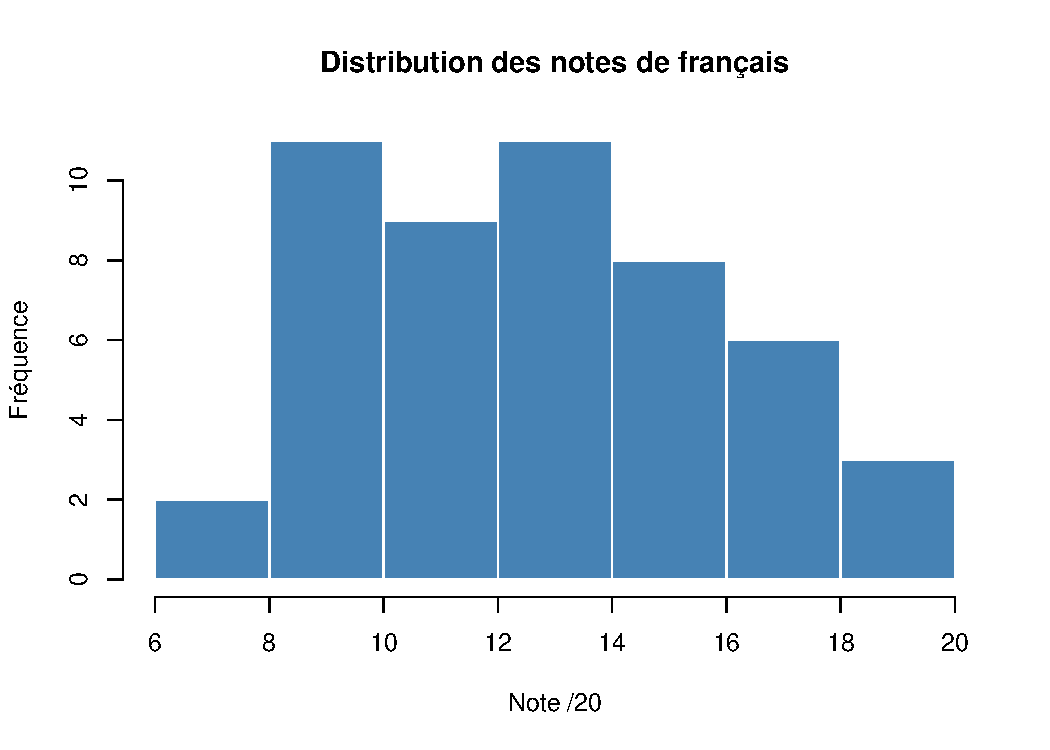
\includegraphics[keepaspectratio]{formation_R_files/figure-pdf/unnamed-chunk-63-1.pdf}}

\begin{Shaded}
\begin{Highlighting}[]
\CommentTok{\# Histogramme avec plus d\textquotesingle{}options}
\FunctionTok{hist}\NormalTok{(enquete\_lycee}\SpecialCharTok{$}\NormalTok{note\_maths,}
     \AttributeTok{main =} \StringTok{"Distribution des notes de mathématiques"}\NormalTok{,}
     \AttributeTok{xlab =} \StringTok{"Note /20"}\NormalTok{,}
     \AttributeTok{ylab =} \StringTok{"Nombre d\textquotesingle{}élèves"}\NormalTok{,}
     \AttributeTok{col =} \StringTok{"coral"}\NormalTok{,}
     \AttributeTok{border =} \StringTok{"white"}\NormalTok{,}
     \AttributeTok{breaks =} \DecValTok{10}\NormalTok{,           }\CommentTok{\# Nombre de classes}
     \AttributeTok{xlim =} \FunctionTok{c}\NormalTok{(}\DecValTok{0}\NormalTok{, }\DecValTok{20}\NormalTok{))       }\CommentTok{\# Limites de l\textquotesingle{}axe X}

\CommentTok{\# Ajouter une ligne de moyenne}
\FunctionTok{abline}\NormalTok{(}\AttributeTok{v =} \FunctionTok{mean}\NormalTok{(enquete\_lycee}\SpecialCharTok{$}\NormalTok{note\_maths), }
       \AttributeTok{col =} \StringTok{"darkred"}\NormalTok{, }\AttributeTok{lwd =} \DecValTok{2}\NormalTok{, }\AttributeTok{lty =} \DecValTok{2}\NormalTok{)}
\FunctionTok{legend}\NormalTok{(}\StringTok{"topright"}\NormalTok{, }\AttributeTok{legend =} \FunctionTok{paste}\NormalTok{(}\StringTok{"Moyenne ="}\NormalTok{, }\FunctionTok{round}\NormalTok{(}\FunctionTok{mean}\NormalTok{(enquete\_lycee}\SpecialCharTok{$}\NormalTok{note\_maths), }\DecValTok{1}\NormalTok{)),}
       \AttributeTok{col =} \StringTok{"darkred"}\NormalTok{, }\AttributeTok{lty =} \DecValTok{2}\NormalTok{, }\AttributeTok{lwd =} \DecValTok{2}\NormalTok{)}
\end{Highlighting}
\end{Shaded}

\pandocbounded{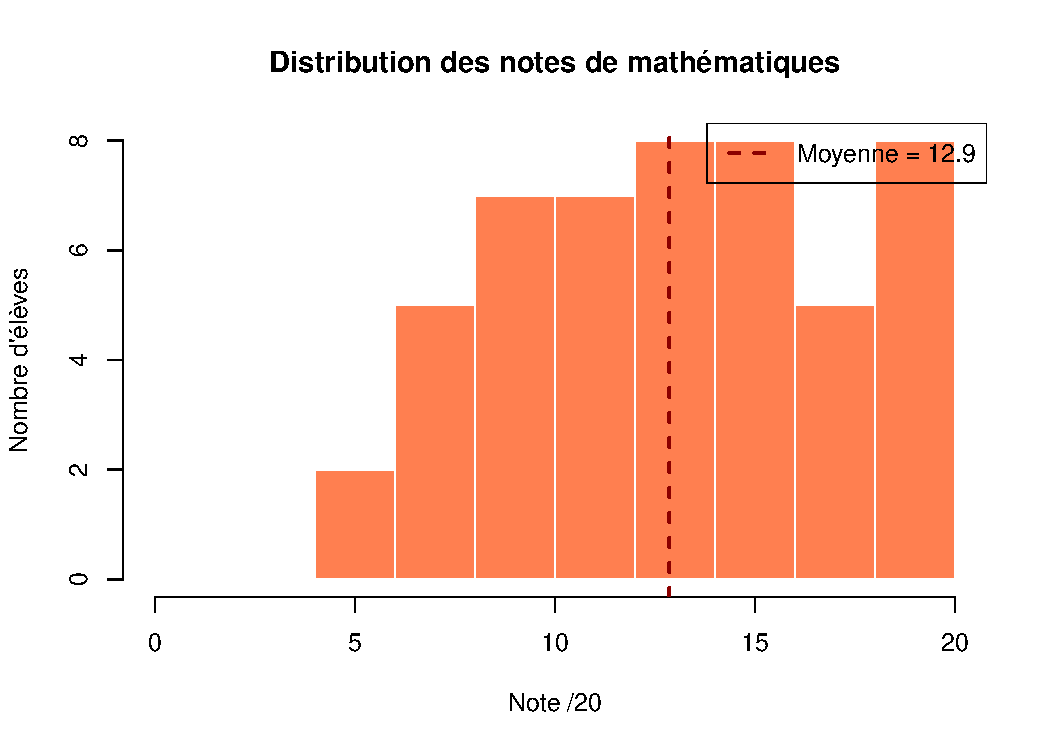
\includegraphics[keepaspectratio]{formation_R_files/figure-pdf/unnamed-chunk-64-1.pdf}}

\subsection{\texorpdfstring{Le diagramme en barres ---
\texttt{barplot()}}{Le diagramme en barres --- barplot()}}\label{le-diagramme-en-barres-barplot}

Le diagramme en barres représente les fréquences ou les valeurs d'une
variable qualitative.

\begin{Shaded}
\begin{Highlighting}[]
\CommentTok{\# Diagramme en barres de la répartition par classe}
\FunctionTok{barplot}\NormalTok{(}\FunctionTok{table}\NormalTok{(enquete\_lycee}\SpecialCharTok{$}\NormalTok{classe),}
        \AttributeTok{main =} \StringTok{"Répartition des élèves par classe"}\NormalTok{,}
        \AttributeTok{xlab =} \StringTok{"Classe"}\NormalTok{,}
        \AttributeTok{ylab =} \StringTok{"Nombre d\textquotesingle{}élèves"}\NormalTok{,}
        \AttributeTok{col =} \FunctionTok{c}\NormalTok{(}\StringTok{"steelblue"}\NormalTok{, }\StringTok{"coral"}\NormalTok{, }\StringTok{"forestgreen"}\NormalTok{),}
        \AttributeTok{border =} \StringTok{"white"}\NormalTok{)}
\end{Highlighting}
\end{Shaded}

\pandocbounded{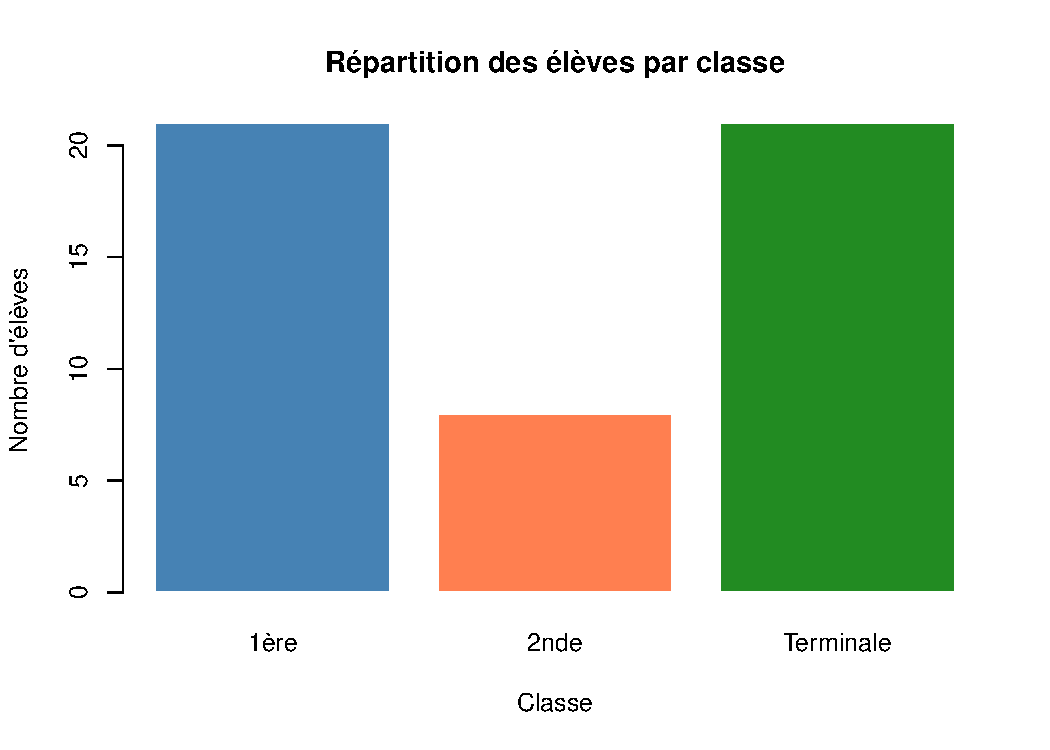
\includegraphics[keepaspectratio]{formation_R_files/figure-pdf/unnamed-chunk-65-1.pdf}}

\begin{Shaded}
\begin{Highlighting}[]
\CommentTok{\# Diagramme en barres groupées (sexe par classe)}
\FunctionTok{barplot}\NormalTok{(}\FunctionTok{table}\NormalTok{(enquete\_lycee}\SpecialCharTok{$}\NormalTok{sexe, enquete\_lycee}\SpecialCharTok{$}\NormalTok{classe),}
        \AttributeTok{beside =} \ConstantTok{TRUE}\NormalTok{,    }\CommentTok{\# Barres côte à côte}
        \AttributeTok{main =} \StringTok{"Répartition par classe et par sexe"}\NormalTok{,}
        \AttributeTok{xlab =} \StringTok{"Classe"}\NormalTok{,}
        \AttributeTok{ylab =} \StringTok{"Nombre d\textquotesingle{}élèves"}\NormalTok{,}
        \AttributeTok{col =} \FunctionTok{c}\NormalTok{(}\StringTok{"steelblue"}\NormalTok{, }\StringTok{"coral"}\NormalTok{),}
        \AttributeTok{border =} \StringTok{"white"}\NormalTok{,}
        \AttributeTok{legend.text =} \FunctionTok{c}\NormalTok{(}\StringTok{"Garçon"}\NormalTok{, }\StringTok{"Fille"}\NormalTok{),}
        \AttributeTok{args.legend =} \FunctionTok{list}\NormalTok{(}\AttributeTok{x =} \StringTok{"topright"}\NormalTok{))}
\end{Highlighting}
\end{Shaded}

\pandocbounded{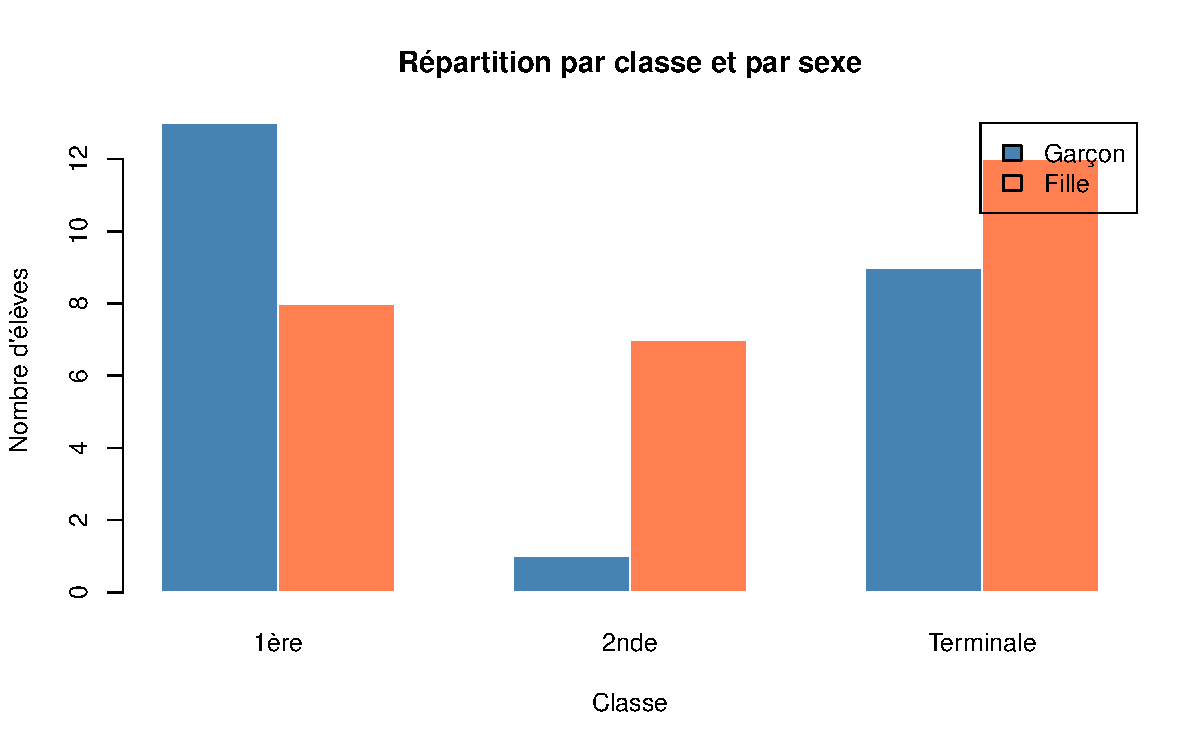
\includegraphics[keepaspectratio]{formation_R_files/figure-pdf/unnamed-chunk-66-1.pdf}}

\begin{tcolorbox}[enhanced jigsaw, arc=.35mm, bottomrule=.15mm, bottomtitle=1mm, breakable, colback=white, colbacktitle=quarto-callout-tip-color!10!white, colframe=quarto-callout-tip-color-frame, coltitle=black, left=2mm, leftrule=.75mm, opacityback=0, opacitybacktitle=0.6, rightrule=.15mm, title=\textcolor{quarto-callout-tip-color}{\faLightbulb}\hspace{0.5em}{Choisir le bon graphique}, titlerule=0mm, toprule=.15mm, toptitle=1mm]

{\def\LTcaptype{none} % do not increment counter
\begin{longtable}[]{@{}
  >{\raggedright\arraybackslash}p{(\linewidth - 2\tabcolsep) * \real{0.4444}}
  >{\raggedright\arraybackslash}p{(\linewidth - 2\tabcolsep) * \real{0.5556}}@{}}
\toprule\noalign{}
\begin{minipage}[b]{\linewidth}\raggedright
Type de variable
\end{minipage} & \begin{minipage}[b]{\linewidth}\raggedright
Graphique recommandé
\end{minipage} \\
\midrule\noalign{}
\endhead
\bottomrule\noalign{}
\endlastfoot
Variable quantitative continue & Histogramme (\texttt{hist}) \\
Variable qualitative & Diagramme en barres (\texttt{barplot}) \\
Deux variables quantitatives & Nuage de points (\texttt{plot}) \\
Évolution dans le temps & Graphique en courbes (\texttt{plot} avec
\texttt{type="l"}) \\
\end{longtable}
}

\end{tcolorbox}

\begin{center}\rule{0.5\linewidth}{0.5pt}\end{center}

\section{Exercices de synthèse}\label{exercices-de-synthuxe8se}

\begin{tcolorbox}[enhanced jigsaw, arc=.35mm, bottomrule=.15mm, bottomtitle=1mm, breakable, colback=white, colbacktitle=quarto-callout-caution-color!10!white, colframe=quarto-callout-caution-color-frame, coltitle=black, left=2mm, leftrule=.75mm, opacityback=0, opacitybacktitle=0.6, rightrule=.15mm, title=\textcolor{quarto-callout-caution-color}{\faFire}\hspace{0.5em}{Exercice 6}, titlerule=0mm, toprule=.15mm, toptitle=1mm]

Calculez dans R les expressions suivantes : 1.
\(\frac{(45 + 38 + 72 + 51)}{4}\) 2. \(\sqrt{(3^2 + 4^2)}\) 3.
\(\frac{1}{1 + e^{-2}}\) (fonction logistique en \(x = 2\))

\end{tcolorbox}

\begin{tcolorbox}[enhanced jigsaw, arc=.35mm, bottomrule=.15mm, bottomtitle=1mm, breakable, colback=white, colbacktitle=quarto-callout-caution-color!10!white, colframe=quarto-callout-caution-color-frame, coltitle=black, left=2mm, leftrule=.75mm, opacityback=0, opacitybacktitle=0.6, rightrule=.15mm, title=\textcolor{quarto-callout-caution-color}{\faFire}\hspace{0.5em}{Exercice 7}, titlerule=0mm, toprule=.15mm, toptitle=1mm]

Créez les variables suivantes et affichez-les : - \texttt{pays} :
``Bénin'' - \texttt{superficie} : 114763 (km²) -
\texttt{population\_2023} : 13352864 - \texttt{pib\_milliards\_usd} :
17.8 - \texttt{membre\_ua} : TRUE

Ensuite, calculez et affichez la densité de population.

\end{tcolorbox}

\begin{tcolorbox}[enhanced jigsaw, arc=.35mm, bottomrule=.15mm, bottomtitle=1mm, breakable, colback=white, colbacktitle=quarto-callout-caution-color!10!white, colframe=quarto-callout-caution-color-frame, coltitle=black, left=2mm, leftrule=.75mm, opacityback=0, opacitybacktitle=0.6, rightrule=.15mm, title=\textcolor{quarto-callout-caution-color}{\faFire}\hspace{0.5em}{Exercice 8}, titlerule=0mm, toprule=.15mm, toptitle=1mm]

On a mesuré la hauteur (en cm) de 10 plants de maïs :
\texttt{128,\ 145,\ 132,\ 118,\ 156,\ 141,\ 129,\ 147,\ 135,\ 122}

\begin{enumerate}
\def\labelenumi{\arabic{enumi}.}
\tightlist
\item
  Créez un vecteur \texttt{hauteurs}
\item
  Calculez la hauteur minimale, maximale, moyenne et médiane
\item
  Combien de plants mesurent plus de 135 cm ? (Indice :
  \texttt{sum(hauteurs\ \textgreater{}\ 135)})
\item
  Calculez l'écart-type
\end{enumerate}

\end{tcolorbox}

\begin{tcolorbox}[enhanced jigsaw, arc=.35mm, bottomrule=.15mm, bottomtitle=1mm, breakable, colback=white, colbacktitle=quarto-callout-caution-color!10!white, colframe=quarto-callout-caution-color-frame, coltitle=black, left=2mm, leftrule=.75mm, opacityback=0, opacitybacktitle=0.6, rightrule=.15mm, title=\textcolor{quarto-callout-caution-color}{\faFire}\hspace{0.5em}{Exercice 9}, titlerule=0mm, toprule=.15mm, toptitle=1mm]

Créez un data frame \texttt{personnel} avec 5 employés :

{\def\LTcaptype{none} % do not increment counter
\begin{longtable}[]{@{}
  >{\raggedright\arraybackslash}p{(\linewidth - 8\tabcolsep) * \real{0.2361}}
  >{\raggedright\arraybackslash}p{(\linewidth - 8\tabcolsep) * \real{0.1944}}
  >{\raggedright\arraybackslash}p{(\linewidth - 8\tabcolsep) * \real{0.2500}}
  >{\raggedright\arraybackslash}p{(\linewidth - 8\tabcolsep) * \real{0.2222}}
  >{\raggedright\arraybackslash}p{(\linewidth - 8\tabcolsep) * \real{0.0972}}@{}}
\toprule\noalign{}
\begin{minipage}[b]{\linewidth}\raggedright
Nom
\end{minipage} & \begin{minipage}[b]{\linewidth}\raggedright
Département
\end{minipage} & \begin{minipage}[b]{\linewidth}\raggedright
Ancienneté (ans)
\end{minipage} & \begin{minipage}[b]{\linewidth}\raggedright
Salaire (FCFA)
\end{minipage} & \begin{minipage}[b]{\linewidth}\raggedright
Cadre
\end{minipage} \\
\midrule\noalign{}
\endhead
\bottomrule\noalign{}
\endlastfoot
AHOYO Bernard & Statistiques & 8 & 450000 & TRUE \\
DOSSOU Clémence & Informatique & 3 & 320000 & FALSE \\
SOSSA Patrick & RH & 12 & 580000 & TRUE \\
KPADA Nathalie & Comptabilité & 5 & 380000 & FALSE \\
AGBO Rémi & Statistiques & 15 & 650000 & TRUE \\
\end{longtable}
}

\begin{enumerate}
\def\labelenumi{\arabic{enumi}.}
\tightlist
\item
  Affichez la structure avec \texttt{str()}
\item
  Quel est le salaire moyen ?
\item
  Quel est le salaire du cadre le plus ancien ?
\item
  Combien d'employés sont cadres ?
\end{enumerate}

\end{tcolorbox}

\begin{tcolorbox}[enhanced jigsaw, arc=.35mm, bottomrule=.15mm, bottomtitle=1mm, breakable, colback=white, colbacktitle=quarto-callout-caution-color!10!white, colframe=quarto-callout-caution-color-frame, coltitle=black, left=2mm, leftrule=.75mm, opacityback=0, opacitybacktitle=0.6, rightrule=.15mm, title=\textcolor{quarto-callout-caution-color}{\faFire}\hspace{0.5em}{Exercice 10}, titlerule=0mm, toprule=.15mm, toptitle=1mm]

Utilisez le data frame \texttt{donnees\_sante} créé en section 7.2.2
pour :

\begin{enumerate}
\def\labelenumi{\arabic{enumi}.}
\tightlist
\item
  Calculer la taille moyenne des patients
\item
  Calculer le poids minimum et maximum
\item
  Créer un tableau de fréquences du sexe
\item
  Calculer les pourcentages par sexe
\item
  Tracer un histogramme de la tension systolique
\end{enumerate}

\end{tcolorbox}

\begin{tcolorbox}[enhanced jigsaw, arc=.35mm, bottomrule=.15mm, bottomtitle=1mm, breakable, colback=white, colbacktitle=quarto-callout-caution-color!10!white, colframe=quarto-callout-caution-color-frame, coltitle=black, left=2mm, leftrule=.75mm, opacityback=0, opacitybacktitle=0.6, rightrule=.15mm, title=\textcolor{quarto-callout-caution-color}{\faFire}\hspace{0.5em}{Exercice 11}, titlerule=0mm, toprule=.15mm, toptitle=1mm]

À partir du vecteur suivant de températures journalières (°C) sur 30
jours :

\begin{Shaded}
\begin{Highlighting}[]
\NormalTok{temperatures }\OtherTok{\textless{}{-}} \FunctionTok{c}\NormalTok{(}\FloatTok{28.5}\NormalTok{, }\FloatTok{31.2}\NormalTok{, }\FloatTok{33.8}\NormalTok{, }\FloatTok{29.4}\NormalTok{, }\FloatTok{35.1}\NormalTok{, }\FloatTok{32.7}\NormalTok{, }\FloatTok{30.1}\NormalTok{, }
                  \FloatTok{34.5}\NormalTok{, }\FloatTok{31.8}\NormalTok{, }\FloatTok{28.9}\NormalTok{, }\FloatTok{36.2}\NormalTok{, }\FloatTok{33.1}\NormalTok{, }\FloatTok{29.7}\NormalTok{, }\FloatTok{31.5}\NormalTok{, }\FloatTok{34.8}\NormalTok{,}
                  \FloatTok{30.3}\NormalTok{, }\FloatTok{32.9}\NormalTok{, }\FloatTok{35.6}\NormalTok{, }\FloatTok{29.1}\NormalTok{, }\FloatTok{33.4}\NormalTok{, }\FloatTok{31.7}\NormalTok{, }\FloatTok{28.3}\NormalTok{, }\FloatTok{34.2}\NormalTok{,}
                  \FloatTok{30.8}\NormalTok{, }\FloatTok{32.1}\NormalTok{, }\FloatTok{35.9}\NormalTok{, }\FloatTok{29.6}\NormalTok{, }\FloatTok{33.7}\NormalTok{, }\FloatTok{31.2}\NormalTok{, }\FloatTok{30.5}\NormalTok{)}
\end{Highlighting}
\end{Shaded}

\begin{enumerate}
\def\labelenumi{\arabic{enumi}.}
\tightlist
\item
  Calculez la température minimale, maximale, moyenne et médiane
\item
  Combien de jours la température a-t-elle dépassé 33°C ?
\item
  Quel est l'écart-type des températures ?
\item
  Tracez un histogramme des températures
\end{enumerate}

\end{tcolorbox}

\begin{tcolorbox}[enhanced jigsaw, arc=.35mm, bottomrule=.15mm, bottomtitle=1mm, breakable, colback=white, colbacktitle=quarto-callout-caution-color!10!white, colframe=quarto-callout-caution-color-frame, coltitle=black, left=2mm, leftrule=.75mm, opacityback=0, opacitybacktitle=0.6, rightrule=.15mm, title=\textcolor{quarto-callout-caution-color}{\faFire}\hspace{0.5em}{Exercice 12}, titlerule=0mm, toprule=.15mm, toptitle=1mm]

Créez un vecteur \texttt{notes\_classe} contenant 20 notes d'élèves
(inventez des valeurs entre 5 et 20), puis :

\begin{enumerate}
\def\labelenumi{\arabic{enumi}.}
\tightlist
\item
  Calculez toutes les statistiques descriptives principales
\item
  Créez un vecteur \texttt{mention} qui indique la mention selon la note
  :

  \begin{itemize}
  \tightlist
  \item
    ``Passable'' si note \textless{} 12
  \item
    ``Assez bien'' si 12 ≤ note \textless{} 14
  \item
    ``Bien'' si 14 ≤ note \textless{} 16
  \item
    ``Très bien'' si note ≥ 16
  \end{itemize}
\item
  Créez un tableau de fréquences des mentions
\end{enumerate}

\end{tcolorbox}

\begin{tcolorbox}[enhanced jigsaw, arc=.35mm, bottomrule=.15mm, bottomtitle=1mm, breakable, colback=white, colbacktitle=quarto-callout-caution-color!10!white, colframe=quarto-callout-caution-color-frame, coltitle=black, left=2mm, leftrule=.75mm, opacityback=0, opacitybacktitle=0.6, rightrule=.15mm, title=\textcolor{quarto-callout-caution-color}{\faFire}\hspace{0.5em}{Exercice 13}, titlerule=0mm, toprule=.15mm, toptitle=1mm]

À partir du data frame \texttt{enquete\_lycee} créé en section 9,
répondez aux questions :

\begin{enumerate}
\def\labelenumi{\arabic{enumi}.}
\tightlist
\item
  Quelle est la note moyenne en français des filles ? (Indice : filtrez
  d'abord les filles)
\item
  Quelle est la note moyenne en maths des garçons ?
\item
  Combien d'élèves étudient plus de 3 heures par jour ?
\item
  Quel pourcentage d'élèves sont en Terminale ?
\end{enumerate}

\end{tcolorbox}

\begin{tcolorbox}[enhanced jigsaw, arc=.35mm, bottomrule=.15mm, bottomtitle=1mm, breakable, colback=white, colbacktitle=quarto-callout-caution-color!10!white, colframe=quarto-callout-caution-color-frame, coltitle=black, left=2mm, leftrule=.75mm, opacityback=0, opacitybacktitle=0.6, rightrule=.15mm, title=\textcolor{quarto-callout-caution-color}{\faFire}\hspace{0.5em}{Exercice 14}, titlerule=0mm, toprule=.15mm, toptitle=1mm]

Créez un diagramme en barres représentant le nombre de communes par
département pour les 5 premiers départements du Bénin :

{\def\LTcaptype{none} % do not increment counter
\begin{longtable}[]{@{}ll@{}}
\toprule\noalign{}
Département & Nb Communes \\
\midrule\noalign{}
\endhead
\bottomrule\noalign{}
\endlastfoot
Alibori & 6 \\
Atacora & 9 \\
Atlantique & 8 \\
Borgou & 12 \\
Collines & 6 \\
\end{longtable}
}

Ajoutez un titre, des labels d'axes et des couleurs différentes pour
chaque barre.

\end{tcolorbox}

\begin{tcolorbox}[enhanced jigsaw, arc=.35mm, bottomrule=.15mm, bottomtitle=1mm, breakable, colback=white, colbacktitle=quarto-callout-caution-color!10!white, colframe=quarto-callout-caution-color-frame, coltitle=black, left=2mm, leftrule=.75mm, opacityback=0, opacitybacktitle=0.6, rightrule=.15mm, title=\textcolor{quarto-callout-caution-color}{\faFire}\hspace{0.5em}{Exercice 15}, titlerule=0mm, toprule=.15mm, toptitle=1mm]

Vous disposez des données suivantes sur la vaccination dans 6 communes :

{\def\LTcaptype{none} % do not increment counter
\begin{longtable}[]{@{}lll@{}}
\toprule\noalign{}
Commune & Cible & Vaccinés \\
\midrule\noalign{}
\endhead
\bottomrule\noalign{}
\endlastfoot
A & 1200 & 1056 \\
B & 850 & 740 \\
C & 2100 & 1890 \\
D & 650 & 598 \\
E & 1800 & 1512 \\
F & 950 & 817 \\
\end{longtable}
}

\begin{enumerate}
\def\labelenumi{\arabic{enumi}.}
\tightlist
\item
  Créez un data frame \texttt{vaccination}
\item
  Calculez le taux de couverture vaccinale pour chaque commune
  (vaccinés/cible × 100)
\item
  Ajoutez cette nouvelle colonne au data frame
\item
  Quelle commune a le meilleur taux de couverture ?
\item
  Tracez un histogramme des taux de couverture
\end{enumerate}

\end{tcolorbox}

\begin{center}\rule{0.5\linewidth}{0.5pt}\end{center}

\section{Corrigés détaillés}\label{corriguxe9s-duxe9tailluxe9s}

\subsection{Corrigé --- Exercice 6}\label{corriguxe9-exercice-6}

\begin{Shaded}
\begin{Highlighting}[]
\CommentTok{\# 1. Calcul de la moyenne de 4 valeurs}
\NormalTok{(}\DecValTok{45} \SpecialCharTok{+} \DecValTok{38} \SpecialCharTok{+} \DecValTok{72} \SpecialCharTok{+} \DecValTok{51}\NormalTok{) }\SpecialCharTok{/} \DecValTok{4}
\end{Highlighting}
\end{Shaded}

\begin{verbatim}
[1] 51.5
\end{verbatim}

\begin{Shaded}
\begin{Highlighting}[]
\CommentTok{\# 2. Hypoténuse (théorème de Pythagore)}
\FunctionTok{sqrt}\NormalTok{(}\DecValTok{3}\SpecialCharTok{\^{}}\DecValTok{2} \SpecialCharTok{+} \DecValTok{4}\SpecialCharTok{\^{}}\DecValTok{2}\NormalTok{)}
\end{Highlighting}
\end{Shaded}

\begin{verbatim}
[1] 5
\end{verbatim}

\begin{Shaded}
\begin{Highlighting}[]
\CommentTok{\# 3. Fonction logistique en x = 2}
\DecValTok{1} \SpecialCharTok{/}\NormalTok{ (}\DecValTok{1} \SpecialCharTok{+} \FunctionTok{exp}\NormalTok{(}\SpecialCharTok{{-}}\DecValTok{2}\NormalTok{))}
\end{Highlighting}
\end{Shaded}

\begin{verbatim}
[1] 0.8807971
\end{verbatim}

\subsection{Corrigé --- Exercice 7}\label{corriguxe9-exercice-7}

\begin{Shaded}
\begin{Highlighting}[]
\CommentTok{\# Création des variables}
\NormalTok{pays }\OtherTok{\textless{}{-}} \StringTok{"Bénin"}
\NormalTok{superficie }\OtherTok{\textless{}{-}} \DecValTok{114763}
\NormalTok{population\_2023 }\OtherTok{\textless{}{-}} \DecValTok{13352864}
\NormalTok{pib\_milliards\_usd }\OtherTok{\textless{}{-}} \FloatTok{17.8}
\NormalTok{membre\_ua }\OtherTok{\textless{}{-}} \ConstantTok{TRUE}

\CommentTok{\# Affichage}
\FunctionTok{cat}\NormalTok{(}\StringTok{"Pays :"}\NormalTok{, pays, }\StringTok{"}\SpecialCharTok{\textbackslash{}n}\StringTok{"}\NormalTok{)}
\end{Highlighting}
\end{Shaded}

\begin{verbatim}
Pays : Bénin 
\end{verbatim}

\begin{Shaded}
\begin{Highlighting}[]
\FunctionTok{cat}\NormalTok{(}\StringTok{"Superficie :"}\NormalTok{, }\FunctionTok{format}\NormalTok{(superficie, }\AttributeTok{big.mark =} \StringTok{" "}\NormalTok{), }\StringTok{"km²}\SpecialCharTok{\textbackslash{}n}\StringTok{"}\NormalTok{)}
\end{Highlighting}
\end{Shaded}

\begin{verbatim}
Superficie : 114 763 km²
\end{verbatim}

\begin{Shaded}
\begin{Highlighting}[]
\FunctionTok{cat}\NormalTok{(}\StringTok{"Population 2023 :"}\NormalTok{, }\FunctionTok{format}\NormalTok{(population\_2023, }\AttributeTok{big.mark =} \StringTok{" "}\NormalTok{), }\StringTok{"}\SpecialCharTok{\textbackslash{}n}\StringTok{"}\NormalTok{)}
\end{Highlighting}
\end{Shaded}

\begin{verbatim}
Population 2023 : 13 352 864 
\end{verbatim}

\begin{Shaded}
\begin{Highlighting}[]
\FunctionTok{cat}\NormalTok{(}\StringTok{"PIB :"}\NormalTok{, pib\_milliards\_usd, }\StringTok{"milliards USD}\SpecialCharTok{\textbackslash{}n}\StringTok{"}\NormalTok{)}
\end{Highlighting}
\end{Shaded}

\begin{verbatim}
PIB : 17.8 milliards USD
\end{verbatim}

\begin{Shaded}
\begin{Highlighting}[]
\FunctionTok{cat}\NormalTok{(}\StringTok{"Membre UA :"}\NormalTok{, membre\_ua, }\StringTok{"}\SpecialCharTok{\textbackslash{}n}\StringTok{"}\NormalTok{)}
\end{Highlighting}
\end{Shaded}

\begin{verbatim}
Membre UA : TRUE 
\end{verbatim}

\begin{Shaded}
\begin{Highlighting}[]
\CommentTok{\# Densité de population}
\NormalTok{densite }\OtherTok{\textless{}{-}}\NormalTok{ population\_2023 }\SpecialCharTok{/}\NormalTok{ superficie}
\FunctionTok{cat}\NormalTok{(}\StringTok{"}\SpecialCharTok{\textbackslash{}n}\StringTok{Densité de population :"}\NormalTok{, }\FunctionTok{round}\NormalTok{(densite, }\DecValTok{1}\NormalTok{), }\StringTok{"habitants/km²}\SpecialCharTok{\textbackslash{}n}\StringTok{"}\NormalTok{)}
\end{Highlighting}
\end{Shaded}

\begin{verbatim}

Densité de population : 116.4 habitants/km²
\end{verbatim}

\subsection{Corrigé --- Exercice 8}\label{corriguxe9-exercice-8}

\begin{Shaded}
\begin{Highlighting}[]
\CommentTok{\# 1. Création du vecteur}
\NormalTok{hauteurs }\OtherTok{\textless{}{-}} \FunctionTok{c}\NormalTok{(}\DecValTok{128}\NormalTok{, }\DecValTok{145}\NormalTok{, }\DecValTok{132}\NormalTok{, }\DecValTok{118}\NormalTok{, }\DecValTok{156}\NormalTok{, }\DecValTok{141}\NormalTok{, }\DecValTok{129}\NormalTok{, }\DecValTok{147}\NormalTok{, }\DecValTok{135}\NormalTok{, }\DecValTok{122}\NormalTok{)}

\CommentTok{\# 2. Statistiques}
\FunctionTok{cat}\NormalTok{(}\StringTok{"Hauteur minimale :"}\NormalTok{, }\FunctionTok{min}\NormalTok{(hauteurs), }\StringTok{"cm}\SpecialCharTok{\textbackslash{}n}\StringTok{"}\NormalTok{)}
\end{Highlighting}
\end{Shaded}

\begin{verbatim}
Hauteur minimale : 118 cm
\end{verbatim}

\begin{Shaded}
\begin{Highlighting}[]
\FunctionTok{cat}\NormalTok{(}\StringTok{"Hauteur maximale :"}\NormalTok{, }\FunctionTok{max}\NormalTok{(hauteurs), }\StringTok{"cm}\SpecialCharTok{\textbackslash{}n}\StringTok{"}\NormalTok{)}
\end{Highlighting}
\end{Shaded}

\begin{verbatim}
Hauteur maximale : 156 cm
\end{verbatim}

\begin{Shaded}
\begin{Highlighting}[]
\FunctionTok{cat}\NormalTok{(}\StringTok{"Hauteur moyenne  :"}\NormalTok{, }\FunctionTok{mean}\NormalTok{(hauteurs), }\StringTok{"cm}\SpecialCharTok{\textbackslash{}n}\StringTok{"}\NormalTok{)}
\end{Highlighting}
\end{Shaded}

\begin{verbatim}
Hauteur moyenne  : 135.3 cm
\end{verbatim}

\begin{Shaded}
\begin{Highlighting}[]
\FunctionTok{cat}\NormalTok{(}\StringTok{"Hauteur médiane  :"}\NormalTok{, }\FunctionTok{median}\NormalTok{(hauteurs), }\StringTok{"cm}\SpecialCharTok{\textbackslash{}n}\StringTok{"}\NormalTok{)}
\end{Highlighting}
\end{Shaded}

\begin{verbatim}
Hauteur médiane  : 133.5 cm
\end{verbatim}

\begin{Shaded}
\begin{Highlighting}[]
\CommentTok{\# 3. Plants de plus de 135 cm}
\NormalTok{nb\_grands }\OtherTok{\textless{}{-}} \FunctionTok{sum}\NormalTok{(hauteurs }\SpecialCharTok{\textgreater{}} \DecValTok{135}\NormalTok{)}
\FunctionTok{cat}\NormalTok{(}\StringTok{"Plants \textgreater{} 135 cm  :"}\NormalTok{, nb\_grands, }\StringTok{"}\SpecialCharTok{\textbackslash{}n}\StringTok{"}\NormalTok{)}
\end{Highlighting}
\end{Shaded}

\begin{verbatim}
Plants > 135 cm  : 4 
\end{verbatim}

\begin{Shaded}
\begin{Highlighting}[]
\CommentTok{\# 4. Écart{-}type}
\FunctionTok{cat}\NormalTok{(}\StringTok{"Écart{-}type       :"}\NormalTok{, }\FunctionTok{round}\NormalTok{(}\FunctionTok{sd}\NormalTok{(hauteurs), }\DecValTok{2}\NormalTok{), }\StringTok{"cm}\SpecialCharTok{\textbackslash{}n}\StringTok{"}\NormalTok{)}
\end{Highlighting}
\end{Shaded}

\begin{verbatim}
Écart-type       : 11.89 cm
\end{verbatim}

\subsection{Corrigé --- Exercice 9}\label{corriguxe9-exercice-9}

\begin{Shaded}
\begin{Highlighting}[]
\CommentTok{\# Création du data frame}
\NormalTok{personnel }\OtherTok{\textless{}{-}} \FunctionTok{data.frame}\NormalTok{(}
  \AttributeTok{nom =} \FunctionTok{c}\NormalTok{(}\StringTok{"AHOYO Bernard"}\NormalTok{, }\StringTok{"DOSSOU Clémence"}\NormalTok{, }\StringTok{"SOSSA Patrick"}\NormalTok{, }\StringTok{"KPADA Nathalie"}\NormalTok{, }\StringTok{"AGBO Rémi"}\NormalTok{),}
  \AttributeTok{departement =} \FunctionTok{c}\NormalTok{(}\StringTok{"Statistiques"}\NormalTok{, }\StringTok{"Informatique"}\NormalTok{, }\StringTok{"RH"}\NormalTok{, }\StringTok{"Comptabilité"}\NormalTok{, }\StringTok{"Statistiques"}\NormalTok{),}
  \AttributeTok{anciennete =} \FunctionTok{c}\NormalTok{(}\DecValTok{8}\NormalTok{, }\DecValTok{3}\NormalTok{, }\DecValTok{12}\NormalTok{, }\DecValTok{5}\NormalTok{, }\DecValTok{15}\NormalTok{),}
  \AttributeTok{salaire =} \FunctionTok{c}\NormalTok{(}\DecValTok{450000}\NormalTok{, }\DecValTok{320000}\NormalTok{, }\DecValTok{580000}\NormalTok{, }\DecValTok{380000}\NormalTok{, }\DecValTok{650000}\NormalTok{),}
  \AttributeTok{cadre =} \FunctionTok{c}\NormalTok{(}\ConstantTok{TRUE}\NormalTok{, }\ConstantTok{FALSE}\NormalTok{, }\ConstantTok{TRUE}\NormalTok{, }\ConstantTok{FALSE}\NormalTok{, }\ConstantTok{TRUE}\NormalTok{)}
\NormalTok{)}

\CommentTok{\# 1. Structure}
\FunctionTok{str}\NormalTok{(personnel)}
\end{Highlighting}
\end{Shaded}

\begin{verbatim}
'data.frame':   5 obs. of  5 variables:
 $ nom        : chr  "AHOYO Bernard" "DOSSOU Clémence" "SOSSA Patrick" "KPADA Nathalie" ...
 $ departement: chr  "Statistiques" "Informatique" "RH" "Comptabilité" ...
 $ anciennete : num  8 3 12 5 15
 $ salaire    : num  450000 320000 580000 380000 650000
 $ cadre      : logi  TRUE FALSE TRUE FALSE TRUE
\end{verbatim}

\begin{Shaded}
\begin{Highlighting}[]
\CommentTok{\# 2. Salaire moyen}
\FunctionTok{cat}\NormalTok{(}\StringTok{"Salaire moyen :"}\NormalTok{, }\FunctionTok{format}\NormalTok{(}\FunctionTok{mean}\NormalTok{(personnel}\SpecialCharTok{$}\NormalTok{salaire), }\AttributeTok{big.mark =} \StringTok{" "}\NormalTok{), }\StringTok{"FCFA}\SpecialCharTok{\textbackslash{}n}\StringTok{"}\NormalTok{)}
\end{Highlighting}
\end{Shaded}

\begin{verbatim}
Salaire moyen : 476 000 FCFA
\end{verbatim}

\begin{Shaded}
\begin{Highlighting}[]
\CommentTok{\# 3. Salaire du cadre le plus ancien}
\NormalTok{cadres }\OtherTok{\textless{}{-}}\NormalTok{ personnel[personnel}\SpecialCharTok{$}\NormalTok{cadre }\SpecialCharTok{==} \ConstantTok{TRUE}\NormalTok{, ]}
\NormalTok{cadre\_plus\_ancien }\OtherTok{\textless{}{-}}\NormalTok{ cadres[}\FunctionTok{which.max}\NormalTok{(cadres}\SpecialCharTok{$}\NormalTok{anciennete), ]}
\FunctionTok{cat}\NormalTok{(}\StringTok{"Cadre le plus ancien :"}\NormalTok{, cadre\_plus\_ancien}\SpecialCharTok{$}\NormalTok{nom, }\StringTok{"}\SpecialCharTok{\textbackslash{}n}\StringTok{"}\NormalTok{)}
\end{Highlighting}
\end{Shaded}

\begin{verbatim}
Cadre le plus ancien : AGBO Rémi 
\end{verbatim}

\begin{Shaded}
\begin{Highlighting}[]
\FunctionTok{cat}\NormalTok{(}\StringTok{"Salaire             :"}\NormalTok{, }\FunctionTok{format}\NormalTok{(cadre\_plus\_ancien}\SpecialCharTok{$}\NormalTok{salaire, }\AttributeTok{big.mark =} \StringTok{" "}\NormalTok{), }\StringTok{"FCFA}\SpecialCharTok{\textbackslash{}n}\StringTok{"}\NormalTok{)}
\end{Highlighting}
\end{Shaded}

\begin{verbatim}
Salaire             : 650 000 FCFA
\end{verbatim}

\begin{Shaded}
\begin{Highlighting}[]
\CommentTok{\# 4. Nombre de cadres}
\FunctionTok{cat}\NormalTok{(}\StringTok{"Nombre de cadres :"}\NormalTok{, }\FunctionTok{sum}\NormalTok{(personnel}\SpecialCharTok{$}\NormalTok{cadre), }\StringTok{"}\SpecialCharTok{\textbackslash{}n}\StringTok{"}\NormalTok{)}
\end{Highlighting}
\end{Shaded}

\begin{verbatim}
Nombre de cadres : 3 
\end{verbatim}

\subsection{Corrigé --- Exercice 10}\label{corriguxe9-exercice-10}

\begin{Shaded}
\begin{Highlighting}[]
\CommentTok{\# Recréer le data frame donnees\_sante}
\FunctionTok{set.seed}\NormalTok{(}\DecValTok{42}\NormalTok{)}
\NormalTok{donnees\_sante }\OtherTok{\textless{}{-}} \FunctionTok{data.frame}\NormalTok{(}
  \AttributeTok{id =} \DecValTok{1}\SpecialCharTok{:}\DecValTok{20}\NormalTok{,}
  \AttributeTok{age =} \FunctionTok{sample}\NormalTok{(}\DecValTok{18}\SpecialCharTok{:}\DecValTok{65}\NormalTok{, }\DecValTok{20}\NormalTok{, }\AttributeTok{replace =} \ConstantTok{TRUE}\NormalTok{),}
  \AttributeTok{sexe =} \FunctionTok{sample}\NormalTok{(}\FunctionTok{c}\NormalTok{(}\StringTok{"Masculin"}\NormalTok{, }\StringTok{"Féminin"}\NormalTok{), }\DecValTok{20}\NormalTok{, }\AttributeTok{replace =} \ConstantTok{TRUE}\NormalTok{),}
  \AttributeTok{poids\_kg =} \FunctionTok{round}\NormalTok{(}\FunctionTok{runif}\NormalTok{(}\DecValTok{20}\NormalTok{, }\DecValTok{45}\NormalTok{, }\DecValTok{95}\NormalTok{), }\DecValTok{1}\NormalTok{),}
  \AttributeTok{taille\_cm =} \FunctionTok{sample}\NormalTok{(}\DecValTok{155}\SpecialCharTok{:}\DecValTok{190}\NormalTok{, }\DecValTok{20}\NormalTok{, }\AttributeTok{replace =} \ConstantTok{TRUE}\NormalTok{),}
  \AttributeTok{tension\_sys =} \FunctionTok{sample}\NormalTok{(}\DecValTok{100}\SpecialCharTok{:}\DecValTok{160}\NormalTok{, }\DecValTok{20}\NormalTok{, }\AttributeTok{replace =} \ConstantTok{TRUE}\NormalTok{)}
\NormalTok{)}

\CommentTok{\# 1. Taille moyenne}
\FunctionTok{cat}\NormalTok{(}\StringTok{"Taille moyenne :"}\NormalTok{, }\FunctionTok{mean}\NormalTok{(donnees\_sante}\SpecialCharTok{$}\NormalTok{taille\_cm), }\StringTok{"cm}\SpecialCharTok{\textbackslash{}n}\StringTok{"}\NormalTok{)}
\end{Highlighting}
\end{Shaded}

\begin{verbatim}
Taille moyenne : 170.7 cm
\end{verbatim}

\begin{Shaded}
\begin{Highlighting}[]
\CommentTok{\# 2. Poids min et max}
\FunctionTok{cat}\NormalTok{(}\StringTok{"Poids minimum  :"}\NormalTok{, }\FunctionTok{min}\NormalTok{(donnees\_sante}\SpecialCharTok{$}\NormalTok{poids\_kg), }\StringTok{"kg}\SpecialCharTok{\textbackslash{}n}\StringTok{"}\NormalTok{)}
\end{Highlighting}
\end{Shaded}

\begin{verbatim}
Poids minimum  : 46.9 kg
\end{verbatim}

\begin{Shaded}
\begin{Highlighting}[]
\FunctionTok{cat}\NormalTok{(}\StringTok{"Poids maximum  :"}\NormalTok{, }\FunctionTok{max}\NormalTok{(donnees\_sante}\SpecialCharTok{$}\NormalTok{poids\_kg), }\StringTok{"kg}\SpecialCharTok{\textbackslash{}n}\StringTok{"}\NormalTok{)}
\end{Highlighting}
\end{Shaded}

\begin{verbatim}
Poids maximum  : 94.1 kg
\end{verbatim}

\begin{Shaded}
\begin{Highlighting}[]
\CommentTok{\# 3. Tableau de fréquences du sexe}
\NormalTok{freq\_sexe }\OtherTok{\textless{}{-}} \FunctionTok{table}\NormalTok{(donnees\_sante}\SpecialCharTok{$}\NormalTok{sexe)}
\FunctionTok{print}\NormalTok{(freq\_sexe)}
\end{Highlighting}
\end{Shaded}

\begin{verbatim}

 Féminin Masculin 
      12        8 
\end{verbatim}

\begin{Shaded}
\begin{Highlighting}[]
\CommentTok{\# 4. Pourcentages par sexe}
\NormalTok{pct\_sexe }\OtherTok{\textless{}{-}} \FunctionTok{round}\NormalTok{(}\FunctionTok{prop.table}\NormalTok{(freq\_sexe) }\SpecialCharTok{*} \DecValTok{100}\NormalTok{, }\DecValTok{1}\NormalTok{)}
\FunctionTok{print}\NormalTok{(pct\_sexe)}
\end{Highlighting}
\end{Shaded}

\begin{verbatim}

 Féminin Masculin 
      60       40 
\end{verbatim}

\begin{Shaded}
\begin{Highlighting}[]
\CommentTok{\# 5. Histogramme de la tension systolique}
\FunctionTok{hist}\NormalTok{(donnees\_sante}\SpecialCharTok{$}\NormalTok{tension\_sys,}
     \AttributeTok{main =} \StringTok{"Distribution de la tension systolique"}\NormalTok{,}
     \AttributeTok{xlab =} \StringTok{"Tension systolique (mmHg)"}\NormalTok{,}
     \AttributeTok{ylab =} \StringTok{"Fréquence"}\NormalTok{,}
     \AttributeTok{col =} \StringTok{"steelblue"}\NormalTok{,}
     \AttributeTok{border =} \StringTok{"white"}\NormalTok{)}
\end{Highlighting}
\end{Shaded}

\pandocbounded{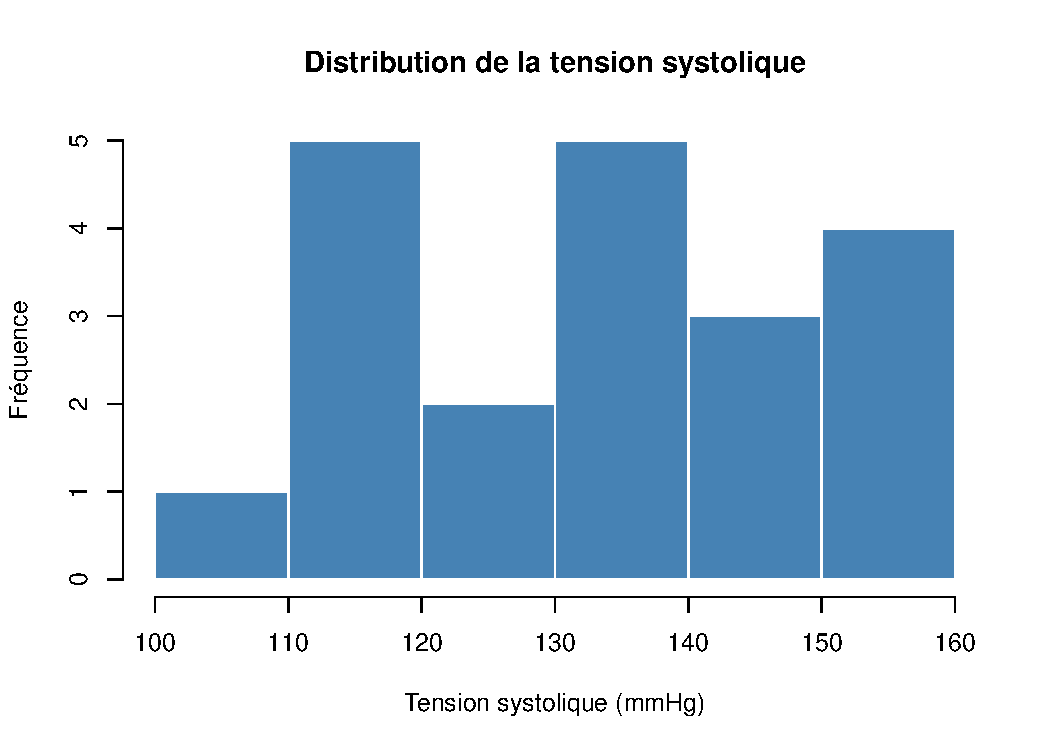
\includegraphics[keepaspectratio]{formation_R_files/figure-pdf/unnamed-chunk-72-1.pdf}}

\subsection{Corrigé --- Exercice 11}\label{corriguxe9-exercice-11}

\begin{Shaded}
\begin{Highlighting}[]
\NormalTok{temperatures }\OtherTok{\textless{}{-}} \FunctionTok{c}\NormalTok{(}\FloatTok{28.5}\NormalTok{, }\FloatTok{31.2}\NormalTok{, }\FloatTok{33.8}\NormalTok{, }\FloatTok{29.4}\NormalTok{, }\FloatTok{35.1}\NormalTok{, }\FloatTok{32.7}\NormalTok{, }\FloatTok{30.1}\NormalTok{, }
                  \FloatTok{34.5}\NormalTok{, }\FloatTok{31.8}\NormalTok{, }\FloatTok{28.9}\NormalTok{, }\FloatTok{36.2}\NormalTok{, }\FloatTok{33.1}\NormalTok{, }\FloatTok{29.7}\NormalTok{, }\FloatTok{31.5}\NormalTok{, }\FloatTok{34.8}\NormalTok{,}
                  \FloatTok{30.3}\NormalTok{, }\FloatTok{32.9}\NormalTok{, }\FloatTok{35.6}\NormalTok{, }\FloatTok{29.1}\NormalTok{, }\FloatTok{33.4}\NormalTok{, }\FloatTok{31.7}\NormalTok{, }\FloatTok{28.3}\NormalTok{, }\FloatTok{34.2}\NormalTok{,}
                  \FloatTok{30.8}\NormalTok{, }\FloatTok{32.1}\NormalTok{, }\FloatTok{35.9}\NormalTok{, }\FloatTok{29.6}\NormalTok{, }\FloatTok{33.7}\NormalTok{, }\FloatTok{31.2}\NormalTok{, }\FloatTok{30.5}\NormalTok{)}

\CommentTok{\# 1. Statistiques principales}
\FunctionTok{cat}\NormalTok{(}\StringTok{"Température minimale :"}\NormalTok{, }\FunctionTok{min}\NormalTok{(temperatures), }\StringTok{"°C}\SpecialCharTok{\textbackslash{}n}\StringTok{"}\NormalTok{)}
\end{Highlighting}
\end{Shaded}

\begin{verbatim}
Température minimale : 28.3 °C
\end{verbatim}

\begin{Shaded}
\begin{Highlighting}[]
\FunctionTok{cat}\NormalTok{(}\StringTok{"Température maximale :"}\NormalTok{, }\FunctionTok{max}\NormalTok{(temperatures), }\StringTok{"°C}\SpecialCharTok{\textbackslash{}n}\StringTok{"}\NormalTok{)}
\end{Highlighting}
\end{Shaded}

\begin{verbatim}
Température maximale : 36.2 °C
\end{verbatim}

\begin{Shaded}
\begin{Highlighting}[]
\FunctionTok{cat}\NormalTok{(}\StringTok{"Température moyenne  :"}\NormalTok{, }\FunctionTok{round}\NormalTok{(}\FunctionTok{mean}\NormalTok{(temperatures), }\DecValTok{2}\NormalTok{), }\StringTok{"°C}\SpecialCharTok{\textbackslash{}n}\StringTok{"}\NormalTok{)}
\end{Highlighting}
\end{Shaded}

\begin{verbatim}
Température moyenne  : 32.02 °C
\end{verbatim}

\begin{Shaded}
\begin{Highlighting}[]
\FunctionTok{cat}\NormalTok{(}\StringTok{"Température médiane  :"}\NormalTok{, }\FunctionTok{median}\NormalTok{(temperatures), }\StringTok{"°C}\SpecialCharTok{\textbackslash{}n}\StringTok{"}\NormalTok{)}
\end{Highlighting}
\end{Shaded}

\begin{verbatim}
Température médiane  : 31.75 °C
\end{verbatim}

\begin{Shaded}
\begin{Highlighting}[]
\CommentTok{\# 2. Jours au{-}dessus de 33°C}
\NormalTok{nb\_jours\_chauds }\OtherTok{\textless{}{-}} \FunctionTok{sum}\NormalTok{(temperatures }\SpecialCharTok{\textgreater{}} \DecValTok{33}\NormalTok{)}
\FunctionTok{cat}\NormalTok{(}\StringTok{"Jours \textgreater{} 33°C :"}\NormalTok{, nb\_jours\_chauds, }\StringTok{"jours sur"}\NormalTok{, }\FunctionTok{length}\NormalTok{(temperatures), }\StringTok{"}\SpecialCharTok{\textbackslash{}n}\StringTok{"}\NormalTok{)}
\end{Highlighting}
\end{Shaded}

\begin{verbatim}
Jours > 33°C : 11 jours sur 30 
\end{verbatim}

\begin{Shaded}
\begin{Highlighting}[]
\CommentTok{\# 3. Écart{-}type}
\FunctionTok{cat}\NormalTok{(}\StringTok{"Écart{-}type :"}\NormalTok{, }\FunctionTok{round}\NormalTok{(}\FunctionTok{sd}\NormalTok{(temperatures), }\DecValTok{2}\NormalTok{), }\StringTok{"°C}\SpecialCharTok{\textbackslash{}n}\StringTok{"}\NormalTok{)}
\end{Highlighting}
\end{Shaded}

\begin{verbatim}
Écart-type : 2.34 °C
\end{verbatim}

\begin{Shaded}
\begin{Highlighting}[]
\CommentTok{\# 4. Histogramme}
\FunctionTok{hist}\NormalTok{(temperatures,}
     \AttributeTok{main =} \StringTok{"Distribution des températures sur 30 jours"}\NormalTok{,}
     \AttributeTok{xlab =} \StringTok{"Température (°C)"}\NormalTok{,}
     \AttributeTok{ylab =} \StringTok{"Nombre de jours"}\NormalTok{,}
     \AttributeTok{col =} \StringTok{"coral"}\NormalTok{,}
     \AttributeTok{border =} \StringTok{"white"}\NormalTok{)}
\FunctionTok{abline}\NormalTok{(}\AttributeTok{v =} \FunctionTok{mean}\NormalTok{(temperatures), }\AttributeTok{col =} \StringTok{"darkred"}\NormalTok{, }\AttributeTok{lwd =} \DecValTok{2}\NormalTok{, }\AttributeTok{lty =} \DecValTok{2}\NormalTok{)}
\end{Highlighting}
\end{Shaded}

\pandocbounded{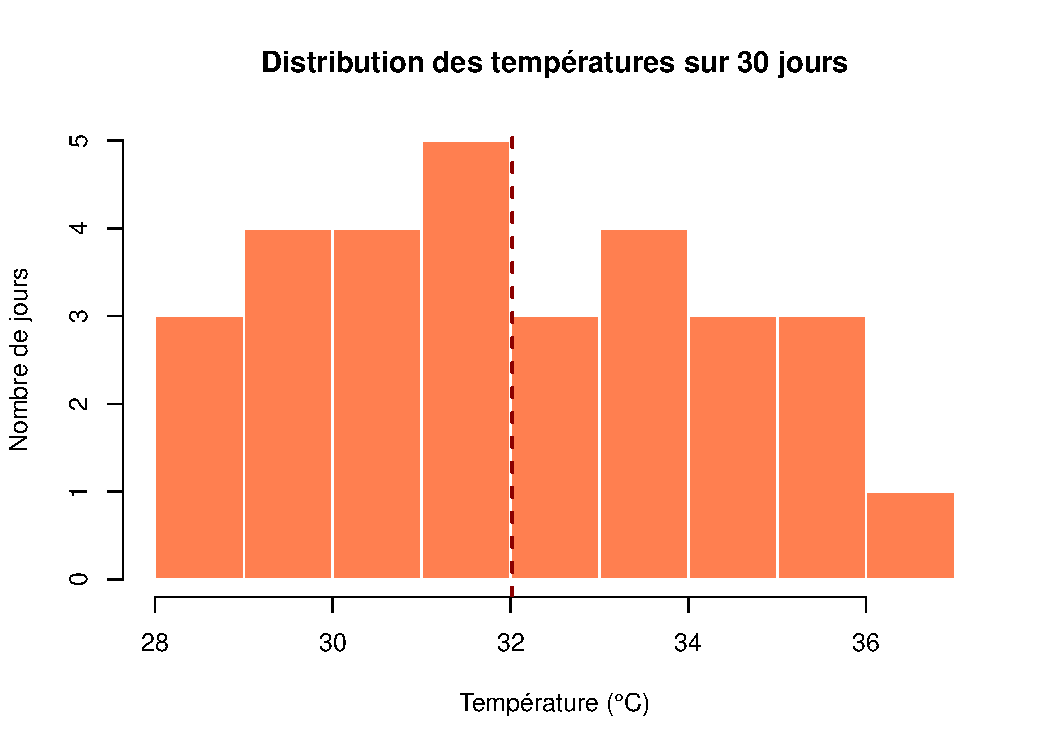
\includegraphics[keepaspectratio]{formation_R_files/figure-pdf/unnamed-chunk-73-1.pdf}}

\subsection{Corrigé --- Exercice 12}\label{corriguxe9-exercice-12}

\begin{Shaded}
\begin{Highlighting}[]
\CommentTok{\# Création d\textquotesingle{}un vecteur de 20 notes}
\FunctionTok{set.seed}\NormalTok{(}\DecValTok{7}\NormalTok{)}
\NormalTok{notes\_classe }\OtherTok{\textless{}{-}} \FunctionTok{c}\NormalTok{(}\DecValTok{8}\NormalTok{, }\DecValTok{14}\NormalTok{, }\DecValTok{17}\NormalTok{, }\DecValTok{11}\NormalTok{, }\DecValTok{15}\NormalTok{, }\DecValTok{9}\NormalTok{, }\DecValTok{16}\NormalTok{, }\DecValTok{12}\NormalTok{, }\DecValTok{7}\NormalTok{, }\DecValTok{18}\NormalTok{,}
                  \DecValTok{13}\NormalTok{, }\DecValTok{10}\NormalTok{, }\DecValTok{15}\NormalTok{, }\DecValTok{6}\NormalTok{, }\DecValTok{14}\NormalTok{, }\DecValTok{11}\NormalTok{, }\DecValTok{19}\NormalTok{, }\DecValTok{12}\NormalTok{, }\DecValTok{16}\NormalTok{, }\DecValTok{8}\NormalTok{)}

\CommentTok{\# 1. Statistiques descriptives}
\FunctionTok{cat}\NormalTok{(}\StringTok{"{-}{-}{-} Statistiques descriptives {-}{-}{-}}\SpecialCharTok{\textbackslash{}n}\StringTok{"}\NormalTok{)}
\end{Highlighting}
\end{Shaded}

\begin{verbatim}
--- Statistiques descriptives ---
\end{verbatim}

\begin{Shaded}
\begin{Highlighting}[]
\FunctionTok{cat}\NormalTok{(}\StringTok{"Minimum    :"}\NormalTok{, }\FunctionTok{min}\NormalTok{(notes\_classe), }\StringTok{"}\SpecialCharTok{\textbackslash{}n}\StringTok{"}\NormalTok{)}
\end{Highlighting}
\end{Shaded}

\begin{verbatim}
Minimum    : 6 
\end{verbatim}

\begin{Shaded}
\begin{Highlighting}[]
\FunctionTok{cat}\NormalTok{(}\StringTok{"Maximum    :"}\NormalTok{, }\FunctionTok{max}\NormalTok{(notes\_classe), }\StringTok{"}\SpecialCharTok{\textbackslash{}n}\StringTok{"}\NormalTok{)}
\end{Highlighting}
\end{Shaded}

\begin{verbatim}
Maximum    : 19 
\end{verbatim}

\begin{Shaded}
\begin{Highlighting}[]
\FunctionTok{cat}\NormalTok{(}\StringTok{"Moyenne    :"}\NormalTok{, }\FunctionTok{mean}\NormalTok{(notes\_classe), }\StringTok{"}\SpecialCharTok{\textbackslash{}n}\StringTok{"}\NormalTok{)}
\end{Highlighting}
\end{Shaded}

\begin{verbatim}
Moyenne    : 12.55 
\end{verbatim}

\begin{Shaded}
\begin{Highlighting}[]
\FunctionTok{cat}\NormalTok{(}\StringTok{"Médiane    :"}\NormalTok{, }\FunctionTok{median}\NormalTok{(notes\_classe), }\StringTok{"}\SpecialCharTok{\textbackslash{}n}\StringTok{"}\NormalTok{)}
\end{Highlighting}
\end{Shaded}

\begin{verbatim}
Médiane    : 12.5 
\end{verbatim}

\begin{Shaded}
\begin{Highlighting}[]
\FunctionTok{cat}\NormalTok{(}\StringTok{"Écart{-}type :"}\NormalTok{, }\FunctionTok{round}\NormalTok{(}\FunctionTok{sd}\NormalTok{(notes\_classe), }\DecValTok{2}\NormalTok{), }\StringTok{"}\SpecialCharTok{\textbackslash{}n}\StringTok{"}\NormalTok{)}
\end{Highlighting}
\end{Shaded}

\begin{verbatim}
Écart-type : 3.78 
\end{verbatim}

\begin{Shaded}
\begin{Highlighting}[]
\CommentTok{\# 2. Attribution des mentions}
\NormalTok{mention }\OtherTok{\textless{}{-}} \FunctionTok{ifelse}\NormalTok{(notes\_classe }\SpecialCharTok{\textless{}} \DecValTok{12}\NormalTok{, }\StringTok{"Passable"}\NormalTok{,}
           \FunctionTok{ifelse}\NormalTok{(notes\_classe }\SpecialCharTok{\textless{}} \DecValTok{14}\NormalTok{, }\StringTok{"Assez bien"}\NormalTok{,}
           \FunctionTok{ifelse}\NormalTok{(notes\_classe }\SpecialCharTok{\textless{}} \DecValTok{16}\NormalTok{, }\StringTok{"Bien"}\NormalTok{, }\StringTok{"Très bien"}\NormalTok{)))}
\NormalTok{mention}
\end{Highlighting}
\end{Shaded}

\begin{verbatim}
 [1] "Passable"   "Bien"       "Très bien"  "Passable"   "Bien"      
 [6] "Passable"   "Très bien"  "Assez bien" "Passable"   "Très bien" 
[11] "Assez bien" "Passable"   "Bien"       "Passable"   "Bien"      
[16] "Passable"   "Très bien"  "Assez bien" "Très bien"  "Passable"  
\end{verbatim}

\begin{Shaded}
\begin{Highlighting}[]
\CommentTok{\# 3. Tableau de fréquences}
\FunctionTok{table}\NormalTok{(mention)}
\end{Highlighting}
\end{Shaded}

\begin{verbatim}
mention
Assez bien       Bien   Passable  Très bien 
         3          4          8          5 
\end{verbatim}

\begin{Shaded}
\begin{Highlighting}[]
\FunctionTok{round}\NormalTok{(}\FunctionTok{prop.table}\NormalTok{(}\FunctionTok{table}\NormalTok{(mention)) }\SpecialCharTok{*} \DecValTok{100}\NormalTok{, }\DecValTok{1}\NormalTok{)}
\end{Highlighting}
\end{Shaded}

\begin{verbatim}
mention
Assez bien       Bien   Passable  Très bien 
        15         20         40         25 
\end{verbatim}

\subsection{Corrigé --- Exercice 13}\label{corriguxe9-exercice-13}

\begin{Shaded}
\begin{Highlighting}[]
\CommentTok{\# Recréer le jeu de données}
\FunctionTok{set.seed}\NormalTok{(}\DecValTok{123}\NormalTok{)}
\NormalTok{n }\OtherTok{\textless{}{-}} \DecValTok{50}
\NormalTok{enquete\_lycee }\OtherTok{\textless{}{-}} \FunctionTok{data.frame}\NormalTok{(}
  \AttributeTok{id =} \DecValTok{1}\SpecialCharTok{:}\NormalTok{n,}
  \AttributeTok{sexe =} \FunctionTok{sample}\NormalTok{(}\FunctionTok{c}\NormalTok{(}\StringTok{"Garçon"}\NormalTok{, }\StringTok{"Fille"}\NormalTok{), n, }\AttributeTok{replace =} \ConstantTok{TRUE}\NormalTok{, }\AttributeTok{prob =} \FunctionTok{c}\NormalTok{(}\FloatTok{0.55}\NormalTok{, }\FloatTok{0.45}\NormalTok{)),}
  \AttributeTok{age =} \FunctionTok{sample}\NormalTok{(}\DecValTok{14}\SpecialCharTok{:}\DecValTok{20}\NormalTok{, n, }\AttributeTok{replace =} \ConstantTok{TRUE}\NormalTok{),}
  \AttributeTok{classe =} \FunctionTok{sample}\NormalTok{(}\FunctionTok{c}\NormalTok{(}\StringTok{"2nde"}\NormalTok{, }\StringTok{"1ère"}\NormalTok{, }\StringTok{"Terminale"}\NormalTok{), n, }\AttributeTok{replace =} \ConstantTok{TRUE}\NormalTok{),}
  \AttributeTok{note\_francais =} \FunctionTok{round}\NormalTok{(}\FunctionTok{runif}\NormalTok{(n, }\DecValTok{6}\NormalTok{, }\DecValTok{19}\NormalTok{), }\DecValTok{1}\NormalTok{),}
  \AttributeTok{note\_maths =} \FunctionTok{round}\NormalTok{(}\FunctionTok{runif}\NormalTok{(n, }\DecValTok{4}\NormalTok{, }\DecValTok{20}\NormalTok{), }\DecValTok{1}\NormalTok{),}
  \AttributeTok{heures\_etude =} \FunctionTok{sample}\NormalTok{(}\DecValTok{1}\SpecialCharTok{:}\DecValTok{6}\NormalTok{, n, }\AttributeTok{replace =} \ConstantTok{TRUE}\NormalTok{)}
\NormalTok{)}

\CommentTok{\# 1. Note moyenne en français des filles}
\NormalTok{filles }\OtherTok{\textless{}{-}}\NormalTok{ enquete\_lycee[enquete\_lycee}\SpecialCharTok{$}\NormalTok{sexe }\SpecialCharTok{==} \StringTok{"Fille"}\NormalTok{, ]}
\FunctionTok{cat}\NormalTok{(}\StringTok{"Moyenne français (Filles)  :"}\NormalTok{, }\FunctionTok{round}\NormalTok{(}\FunctionTok{mean}\NormalTok{(filles}\SpecialCharTok{$}\NormalTok{note\_francais), }\DecValTok{2}\NormalTok{), }\StringTok{"}\SpecialCharTok{\textbackslash{}n}\StringTok{"}\NormalTok{)}
\end{Highlighting}
\end{Shaded}

\begin{verbatim}
Moyenne français (Filles)  : 13 
\end{verbatim}

\begin{Shaded}
\begin{Highlighting}[]
\CommentTok{\# 2. Note moyenne en maths des garçons}
\NormalTok{garcons }\OtherTok{\textless{}{-}}\NormalTok{ enquete\_lycee[enquete\_lycee}\SpecialCharTok{$}\NormalTok{sexe }\SpecialCharTok{==} \StringTok{"Garçon"}\NormalTok{, ]}
\FunctionTok{cat}\NormalTok{(}\StringTok{"Moyenne maths (Garçons)    :"}\NormalTok{, }\FunctionTok{round}\NormalTok{(}\FunctionTok{mean}\NormalTok{(garcons}\SpecialCharTok{$}\NormalTok{note\_maths), }\DecValTok{2}\NormalTok{), }\StringTok{"}\SpecialCharTok{\textbackslash{}n}\StringTok{"}\NormalTok{)}
\end{Highlighting}
\end{Shaded}

\begin{verbatim}
Moyenne maths (Garçons)    : 12.79 
\end{verbatim}

\begin{Shaded}
\begin{Highlighting}[]
\CommentTok{\# 3. Élèves étudiant plus de 3h par jour}
\NormalTok{nb\_studieux }\OtherTok{\textless{}{-}} \FunctionTok{sum}\NormalTok{(enquete\_lycee}\SpecialCharTok{$}\NormalTok{heures\_etude }\SpecialCharTok{\textgreater{}} \DecValTok{3}\NormalTok{)}
\FunctionTok{cat}\NormalTok{(}\StringTok{"Élèves étudiant \textgreater{} 3h/jour :"}\NormalTok{, nb\_studieux, }\StringTok{"}\SpecialCharTok{\textbackslash{}n}\StringTok{"}\NormalTok{)}
\end{Highlighting}
\end{Shaded}

\begin{verbatim}
Élèves étudiant > 3h/jour : 22 
\end{verbatim}

\begin{Shaded}
\begin{Highlighting}[]
\CommentTok{\# 4. Pourcentage en Terminale}
\NormalTok{pct\_terminale }\OtherTok{\textless{}{-}} \FunctionTok{mean}\NormalTok{(enquete\_lycee}\SpecialCharTok{$}\NormalTok{classe }\SpecialCharTok{==} \StringTok{"Terminale"}\NormalTok{) }\SpecialCharTok{*} \DecValTok{100}
\FunctionTok{cat}\NormalTok{(}\StringTok{"\% en Terminale            :"}\NormalTok{, }\FunctionTok{round}\NormalTok{(pct\_terminale, }\DecValTok{1}\NormalTok{), }\StringTok{"\%}\SpecialCharTok{\textbackslash{}n}\StringTok{"}\NormalTok{)}
\end{Highlighting}
\end{Shaded}

\begin{verbatim}
% en Terminale            : 42 %
\end{verbatim}

\subsection{Corrigé --- Exercice 14}\label{corriguxe9-exercice-14}

\begin{Shaded}
\begin{Highlighting}[]
\CommentTok{\# Données des communes par département}
\NormalTok{departements }\OtherTok{\textless{}{-}} \FunctionTok{c}\NormalTok{(}\StringTok{"Alibori"}\NormalTok{, }\StringTok{"Atacora"}\NormalTok{, }\StringTok{"Atlantique"}\NormalTok{, }\StringTok{"Borgou"}\NormalTok{, }\StringTok{"Collines"}\NormalTok{)}
\NormalTok{nb\_communes }\OtherTok{\textless{}{-}} \FunctionTok{c}\NormalTok{(}\DecValTok{6}\NormalTok{, }\DecValTok{9}\NormalTok{, }\DecValTok{8}\NormalTok{, }\DecValTok{12}\NormalTok{, }\DecValTok{6}\NormalTok{)}
\NormalTok{couleurs }\OtherTok{\textless{}{-}} \FunctionTok{c}\NormalTok{(}\StringTok{"steelblue"}\NormalTok{, }\StringTok{"coral"}\NormalTok{, }\StringTok{"forestgreen"}\NormalTok{, }\StringTok{"gold"}\NormalTok{, }\StringTok{"mediumpurple"}\NormalTok{)}

\CommentTok{\# Diagramme en barres}
\FunctionTok{barplot}\NormalTok{(nb\_communes,}
        \AttributeTok{names.arg =}\NormalTok{ departements,}
        \AttributeTok{main =} \StringTok{"Nombre de communes par département (Bénin)"}\NormalTok{,}
        \AttributeTok{xlab =} \StringTok{"Département"}\NormalTok{,}
        \AttributeTok{ylab =} \StringTok{"Nombre de communes"}\NormalTok{,}
        \AttributeTok{col =}\NormalTok{ couleurs,}
        \AttributeTok{border =} \StringTok{"white"}\NormalTok{,}
        \AttributeTok{ylim =} \FunctionTok{c}\NormalTok{(}\DecValTok{0}\NormalTok{, }\DecValTok{15}\NormalTok{))}

\CommentTok{\# Ajouter les valeurs sur les barres}
\FunctionTok{text}\NormalTok{(}\AttributeTok{x =} \FunctionTok{barplot}\NormalTok{(nb\_communes, }\AttributeTok{plot =} \ConstantTok{FALSE}\NormalTok{),}
     \AttributeTok{y =}\NormalTok{ nb\_communes }\SpecialCharTok{+} \FloatTok{0.3}\NormalTok{,}
     \AttributeTok{labels =}\NormalTok{ nb\_communes,}
     \AttributeTok{cex =} \FloatTok{0.9}\NormalTok{, }\AttributeTok{font =} \DecValTok{2}\NormalTok{)}
\end{Highlighting}
\end{Shaded}

\pandocbounded{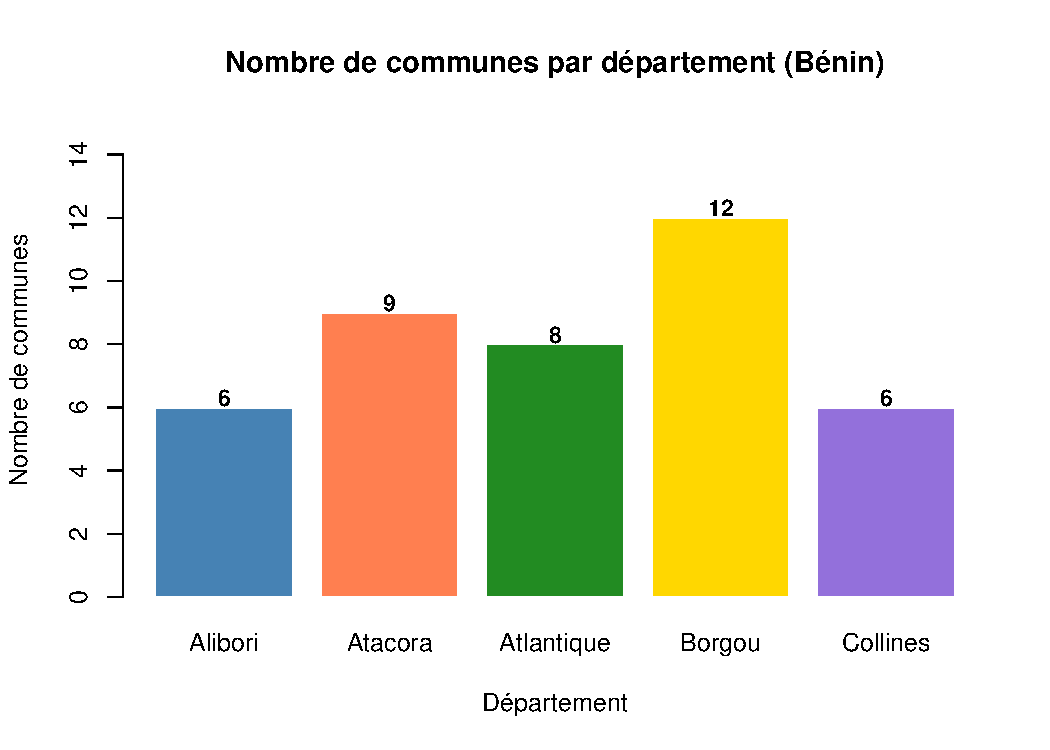
\includegraphics[keepaspectratio]{formation_R_files/figure-pdf/unnamed-chunk-76-1.pdf}}

\subsection{Corrigé --- Exercice 15}\label{corriguxe9-exercice-15}

\begin{Shaded}
\begin{Highlighting}[]
\CommentTok{\# 1. Création du data frame}
\NormalTok{vaccination }\OtherTok{\textless{}{-}} \FunctionTok{data.frame}\NormalTok{(}
  \AttributeTok{commune =} \FunctionTok{c}\NormalTok{(}\StringTok{"A"}\NormalTok{, }\StringTok{"B"}\NormalTok{, }\StringTok{"C"}\NormalTok{, }\StringTok{"D"}\NormalTok{, }\StringTok{"E"}\NormalTok{, }\StringTok{"F"}\NormalTok{),}
  \AttributeTok{cible =} \FunctionTok{c}\NormalTok{(}\DecValTok{1200}\NormalTok{, }\DecValTok{850}\NormalTok{, }\DecValTok{2100}\NormalTok{, }\DecValTok{650}\NormalTok{, }\DecValTok{1800}\NormalTok{, }\DecValTok{950}\NormalTok{),}
  \AttributeTok{vaccines =} \FunctionTok{c}\NormalTok{(}\DecValTok{1056}\NormalTok{, }\DecValTok{740}\NormalTok{, }\DecValTok{1890}\NormalTok{, }\DecValTok{598}\NormalTok{, }\DecValTok{1512}\NormalTok{, }\DecValTok{817}\NormalTok{)}
\NormalTok{)}

\CommentTok{\# 2. Calcul du taux de couverture}
\NormalTok{vaccination}\SpecialCharTok{$}\NormalTok{taux\_couverture }\OtherTok{\textless{}{-}} \FunctionTok{round}\NormalTok{((vaccination}\SpecialCharTok{$}\NormalTok{vaccines }\SpecialCharTok{/}\NormalTok{ vaccination}\SpecialCharTok{$}\NormalTok{cible) }\SpecialCharTok{*} \DecValTok{100}\NormalTok{, }\DecValTok{1}\NormalTok{)}

\CommentTok{\# 3. Afficher le data frame avec la nouvelle colonne}
\FunctionTok{print}\NormalTok{(vaccination)}
\end{Highlighting}
\end{Shaded}

\begin{verbatim}
  commune cible vaccines taux_couverture
1       A  1200     1056            88.0
2       B   850      740            87.1
3       C  2100     1890            90.0
4       D   650      598            92.0
5       E  1800     1512            84.0
6       F   950      817            86.0
\end{verbatim}

\begin{Shaded}
\begin{Highlighting}[]
\CommentTok{\# 4. Commune avec le meilleur taux}
\NormalTok{meilleure\_commune }\OtherTok{\textless{}{-}}\NormalTok{ vaccination[}\FunctionTok{which.max}\NormalTok{(vaccination}\SpecialCharTok{$}\NormalTok{taux\_couverture), ]}
\FunctionTok{cat}\NormalTok{(}\StringTok{"}\SpecialCharTok{\textbackslash{}n}\StringTok{Meilleure couverture :"}\NormalTok{, meilleure\_commune}\SpecialCharTok{$}\NormalTok{commune,}
    \StringTok{"avec"}\NormalTok{, meilleure\_commune}\SpecialCharTok{$}\NormalTok{taux\_couverture, }\StringTok{"\%}\SpecialCharTok{\textbackslash{}n}\StringTok{"}\NormalTok{)}
\end{Highlighting}
\end{Shaded}

\begin{verbatim}

Meilleure couverture : D avec 92 %
\end{verbatim}

\begin{Shaded}
\begin{Highlighting}[]
\CommentTok{\# 5. Histogramme des taux}
\FunctionTok{hist}\NormalTok{(vaccination}\SpecialCharTok{$}\NormalTok{taux\_couverture,}
     \AttributeTok{main =} \StringTok{"Distribution des taux de couverture vaccinale"}\NormalTok{,}
     \AttributeTok{xlab =} \StringTok{"Taux de couverture (\%)"}\NormalTok{,}
     \AttributeTok{ylab =} \StringTok{"Nombre de communes"}\NormalTok{,}
     \AttributeTok{col =} \StringTok{"steelblue"}\NormalTok{,}
     \AttributeTok{border =} \StringTok{"white"}\NormalTok{,}
     \AttributeTok{breaks =} \DecValTok{5}\NormalTok{,}
     \AttributeTok{xlim =} \FunctionTok{c}\NormalTok{(}\DecValTok{80}\NormalTok{, }\DecValTok{100}\NormalTok{))}
\end{Highlighting}
\end{Shaded}

\pandocbounded{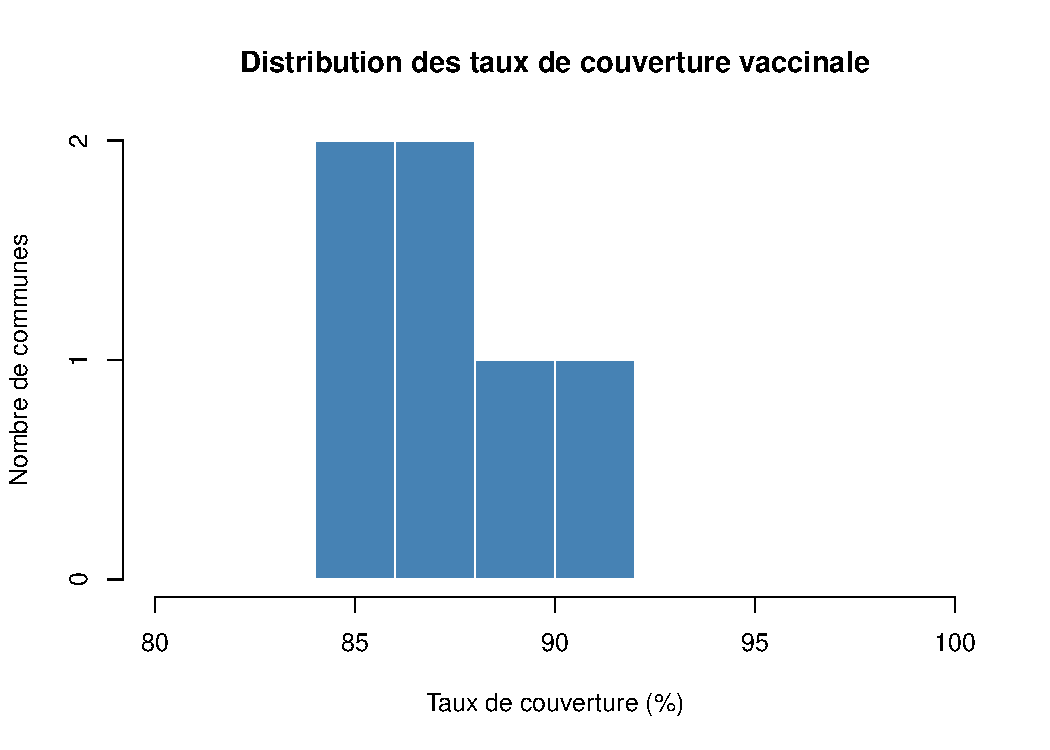
\includegraphics[keepaspectratio]{formation_R_files/figure-pdf/unnamed-chunk-77-1.pdf}}

\begin{center}\rule{0.5\linewidth}{0.5pt}\end{center}

\section*{Conclusion}\label{conclusion}
\addcontentsline{toc}{section}{Conclusion}

\subsection{Résumé des notions
apprises}\label{ruxe9sumuxe9-des-notions-apprises}

Félicitations ! À l'issue de cette première séance, vous avez acquis les
bases essentielles pour travailler avec R.

\begin{tcolorbox}[enhanced jigsaw, arc=.35mm, bottomrule=.15mm, bottomtitle=1mm, breakable, colback=white, colbacktitle=quarto-callout-note-color!10!white, colframe=quarto-callout-note-color-frame, coltitle=black, left=2mm, leftrule=.75mm, opacityback=0, opacitybacktitle=0.6, rightrule=.15mm, title=\textcolor{quarto-callout-note-color}{\faInfo}\hspace{0.5em}{Ce que vous avez appris aujourd'hui}, titlerule=0mm, toprule=.15mm, toptitle=1mm]

\textbf{Environnement de travail}

\begin{itemize}
\tightlist
\item
  Installer R et RStudio
\item
  Naviguer dans l'interface à 4 panneaux de RStudio
\item
  Créer, éditer et sauvegarder un script R
\end{itemize}

\textbf{Programmation de base}

\begin{itemize}
\tightlist
\item
  Écrire des commandes et des commentaires dans R
\item
  Réaliser des calculs arithmétiques (+, -, *, /, \^{}, sqrt)
\item
  Créer et manipuler des variables avec l'opérateur
  \texttt{\textless{}-}
\item
  Utiliser \texttt{ls()} et \texttt{rm()} pour gérer l'environnement
\end{itemize}

\textbf{Types de données}

\begin{itemize}
\tightlist
\item
  Distinguer les types : numérique, caractère, logique
\item
  Utiliser \texttt{class()} et \texttt{typeof()} pour identifier les
  types
\item
  Convertir entre types (\texttt{as.numeric()}, \texttt{as.character()},
  etc.)
\end{itemize}

\textbf{Structures de données}

\begin{itemize}
\tightlist
\item
  Créer et manipuler des vecteurs avec \texttt{c()}
\item
  Créer et explorer des data frames avec \texttt{data.frame()}
\item
  Utiliser \texttt{head()}, \texttt{tail()}, \texttt{str()},
  \texttt{summary()}
\end{itemize}

\textbf{Analyse de données}

\begin{itemize}
\tightlist
\item
  Importer des données Excel avec \texttt{readxl}
\item
  Calculer des statistiques descriptives (mean, median, sd, table,
  prop.table)
\item
  Produire des graphiques de base (hist, barplot)
\end{itemize}

\end{tcolorbox}

\begin{center}\rule{0.5\linewidth}{0.5pt}\end{center}

\section*{Travail personnel}\label{travail-personnel}
\addcontentsline{toc}{section}{Travail personnel}

Avant la prochaine séance, réalisez les exercices suivants à la maison
pour consolider vos acquis.

\begin{tcolorbox}[enhanced jigsaw, arc=.35mm, bottomrule=.15mm, bottomtitle=1mm, breakable, colback=white, colbacktitle=quarto-callout-caution-color!10!white, colframe=quarto-callout-caution-color-frame, coltitle=black, left=2mm, leftrule=.75mm, opacityback=0, opacitybacktitle=0.6, rightrule=.15mm, title=\textcolor{quarto-callout-caution-color}{\faFire}\hspace{0.5em}{Devoir à rendre --- Exercice A : Script annoté}, titlerule=0mm, toprule=.15mm, toptitle=1mm]

Créez un script R nommé \texttt{devoir\_seance1.R} contenant :

\begin{enumerate}
\def\labelenumi{\arabic{enumi}.}
\tightlist
\item
  Un en-tête complet (nom, date, objectif)
\item
  La création d'un data frame \texttt{eleves\_ecole} avec au moins 8
  élèves et 5 variables de votre choix (nom, classe, sexe, note1, note2)
\item
  Le calcul de la moyenne de chaque note
\item
  L'identification de l'élève avec la meilleure moyenne
\item
  Un tableau de fréquences et de pourcentages par classe
\item
  Un histogramme de la distribution des notes
\item
  Des commentaires expliquant chaque étape
\end{enumerate}

\end{tcolorbox}

\begin{tcolorbox}[enhanced jigsaw, arc=.35mm, bottomrule=.15mm, bottomtitle=1mm, breakable, colback=white, colbacktitle=quarto-callout-caution-color!10!white, colframe=quarto-callout-caution-color-frame, coltitle=black, left=2mm, leftrule=.75mm, opacityback=0, opacitybacktitle=0.6, rightrule=.15mm, title=\textcolor{quarto-callout-caution-color}{\faFire}\hspace{0.5em}{Devoir à rendre --- Exercice B : Exploration}, titlerule=0mm, toprule=.15mm, toptitle=1mm]

Collectez (ou inventez) des données sur votre environnement proche
(votre classe, votre quartier, votre famille) et créez un mini-jeu de
données d'au moins 10 lignes.

Réalisez une analyse descriptive complète et produisez au moins 2
graphiques commentés.

\end{tcolorbox}

\begin{tcolorbox}[enhanced jigsaw, arc=.35mm, bottomrule=.15mm, bottomtitle=1mm, breakable, colback=white, colbacktitle=quarto-callout-tip-color!10!white, colframe=quarto-callout-tip-color-frame, coltitle=black, left=2mm, leftrule=.75mm, opacityback=0, opacitybacktitle=0.6, rightrule=.15mm, title=\textcolor{quarto-callout-tip-color}{\faLightbulb}\hspace{0.5em}{Ressources pour aller plus loin}, titlerule=0mm, toprule=.15mm, toptitle=1mm]

\textbf{Documentation officielle}

\begin{itemize}
\tightlist
\item
  Site officiel R : \url{https://www.r-project.org}
\item
  Aide intégrée RStudio : tapez \texttt{?nom\_fonction} dans la console
  (ex: \texttt{?mean})
\end{itemize}

\textbf{Tutoriels en ligne gratuits}

\begin{itemize}
\tightlist
\item
  \href{https://r4ds.hadley.nz}{R for Data Science (en français)} ---
  Bible de l'analyse de données avec R
\item
  \href{https://juba.github.io/tidyverse/}{Introduction à R et au
  tidyverse} --- Excellent tutoriel en français
\item
  Swirl : package interactif d'apprentissage de R (tapez
  \texttt{install.packages("swirl")})
\end{itemize}

\textbf{Communauté}

\begin{itemize}
\tightlist
\item
  Stack Overflow :
  \href{https://stackoverflow.com/questions/tagged/r}{stackoverflow.com/questions/tagged/r}
\item
  R-bloggers : \href{https://www.r-bloggers.com}{r-bloggers.com}
\end{itemize}

\end{tcolorbox}

\begin{tcolorbox}[enhanced jigsaw, arc=.35mm, bottomrule=.15mm, bottomtitle=1mm, breakable, colback=white, colbacktitle=quarto-callout-note-color!10!white, colframe=quarto-callout-note-color-frame, coltitle=black, left=2mm, leftrule=.75mm, opacityback=0, opacitybacktitle=0.6, rightrule=.15mm, title=\textcolor{quarto-callout-note-color}{\faInfo}\hspace{0.5em}{Aperçu de la Séance 2}, titlerule=0mm, toprule=.15mm, toptitle=1mm]

La prochaine séance couvrira :

\begin{itemize}
\tightlist
\item
  Le package \textbf{tidyverse} : manipulation avancée de données avec
  \texttt{dplyr} et \texttt{tidyr}
\item
  Les graphiques avec \textbf{ggplot2} : visualisations professionnelles
  et personnalisées
\item
  La gestion des valeurs manquantes (\texttt{NA})
\item
  La création de fonctions personnalisées
\item
  Introduction aux boucles et à la programmation itérative
\end{itemize}

\end{tcolorbox}

\begin{center}\rule{0.5\linewidth}{0.5pt}\end{center}




\end{document}
